\documentclass[12pt, a4paper]{report}

% ==================================================
% PREAMBLE
% ==================================================




\usepackage{amssymb}
\usepackage{array}
\usepackage[utf8]{inputenc}   % Text encoding
\usepackage[T1]{fontenc}      % Font encoding
\usepackage{mathptmx}         % Times New Roman font
\usepackage{geometry}         % Margins
\usepackage{setspace}         % Line spacing
\usepackage{titlesec}         % Heading formatting
\usepackage{hyperref}         % PDF Links
\usepackage{caption}          % Figure captions
\usepackage{float}            % Figure placement
\usepackage{amsmath}          % Math
\usepackage{booktabs}         % Tables
\usepackage{tabularx}
\usepackage{tasks}
\usepackage{enumitem}
\usepackage[export]{adjustbox}
\usepackage{graphicx} 
\usepackage{subcaption}
\setcounter{secnumdepth}{3} % This puts the number (2.4.1.1) in the text
\setcounter{tocdepth}{3} % This forces subsubsections to appear in the Table of Contents
\usepackage{hyperref}
\hypersetup{
    colorlinks=true,   % This removes the boxes and colors the text instead
    linkcolor=blue,    % This makes your Table of Contents links blue
    filecolor=magenta,      
    urlcolor=cyan,
    pdftitle={Overleaf Example},
    pdfpagemode=FullScreen,
}
\usepackage{listings}
\usepackage{xcolor}


% Define Verilog-A colors
\definecolor{vcomment}{rgb}{0, 0.5, 0}
\definecolor{vkeyword}{rgb}{0, 0, 1}
\definecolor{vstring}{rgb}{0.6, 0.1, 0.1}

\lstset{
    language=Verilog, % Verilog is the closest base for Verilog-A
    basicstyle=\ttfamily\small,
    keywordstyle=\color{vkeyword}\bfseries,
    commentstyle=\color{vcomment},
    stringstyle=\color{vstring},
    numbers=left,
    numberstyle=\tiny\color{gray},
    stepnumber=1,
    breaklines=true,
    frame=single,
    tabsize=4,
    captionpos=b,
    showstringspaces=false
}

% Custom commands for formatting
\newcommand{\Hz}{\text{Hz}}
\newcommand{\GHz}{\text{GHz}}
\newcommand{\Gbps}{\text{Gbps}}
\newcommand{\ps}{\text{ps}}
\newcommand{\mV}{\text{mV}}
\newcommand{\mA}{\text{mA}}
\newcommand{\UI}{\text{UI}}
\newcommand{\BER}{\text{BER}}
\newcommand{\RMS}{\text{RMS}}
\newcommand{\TJ}{T_j}
\renewcommand{\DJ}{D_j}
\newcommand{\RJ}{R_j}
\newcommand{\DCD}{\text{DCD}}
\newcommand{\ISI}{\text{ISI}}
\newcommand{\BUJ}{\text{BUJ}}
\newcommand{\DCC}{\text{DCC}}
\newcommand{\PLL}{\text{PLL}}





% Standard Margins
\geometry{left=30mm, right=25mm, top=25mm, bottom=25mm}

% 1.5 Spacing
\onehalfspacing

\renewcommand{\thesection}{\thechapter.\arabic{section}}
\renewcommand{\thesubsection}{\thesection.\arabic{subsection}}
\renewcommand{\thesubsubsection}{\thesubsection.\arabic{subsubsection}}


\begin{document}

% ==================================================
% FRONT MATTER
% ==================================================
\title{\textbf{High-Speed SerDes Transmitter Design in 22nm FD-SOI}}

\maketitle

% This generates your "Outline" , "Table of Contents" automatically
\tableofcontents
\newpage

%\listoftables 
%\newpage
% ==================================================
% CHAPTER 1: INTRODUCTION
% ==================================================
\chapter{Introduction}
\label{ch:intro}

\section{Historical Evolution: From Parallel to Serial}
    \subsection{The Legacy of Parallel PCI}
    \subsection{The Shift to Serial PCIe}
    
   
\section{PCIe Standard Overview}
    \subsection{Evolution of PCIe Generations}
    \subsection{Protocol Architecture}
    \subsection{PCIe 6.0 Innovations}
    \subsection{PAM4 Signaling Fundamentals}
        \subsubsection{SNR Trade-offs and Linearity Requirements}
        \subsubsection{Forward Error Correction (FEC) Implications}

\section{Thesis Objectives and Contributions}
\section{Thesis Organization}

% ==================================================
% CHAPTER 2: FUNDAMENTALS & LIT REVIEW
% ==================================================
\chapter{System overview and Literature Architectures}
\label{ch:fundamentals}

\section{Clocking Systems in Wireline Transceivers}
\label{sec:clocking-systems}

In high-speed wireline communication, the clocking system is the "heartbeat" of the entire transceiver. Its primary function is to provide a precise time reference that dictates when data bits are generated, transmitted, and sampled. Without a highly stable clock, the synchronization between the transmitter (TX) Blocks would fail, leading to massive data corruption.

\subsection{The Role of Clocking in Serialization}
\label{subsec:role-clocking-serialization}

The most critical application of high-speed clocking within the transmitter is the \textbf{Serialization process}. In modern systems, data is processed internally in a parallel format (e.g., 32 or 64 bits wide) at a relatively low frequency to save power. To transmit this data over a single physical channel (like a copper trace or fiber), it must be converted into a serial bitstream.

The Serializer uses the clock signal to "multiplex" these parallel bits into a single high-speed line. For example, in a system aiming for a 64 Gbps data rate with 32Gbaud, the clocking network must provide timing edges that allow the serializer to place a new bit every \textbf{31.25 picoseconds}. Any misalignment or instability in this clock directly reduces the "eye opening" of the transmitted signal, making it harder for the receiver to distinguish between a digital '0' and '1'.

\begin{figure}[H]
    \centering
    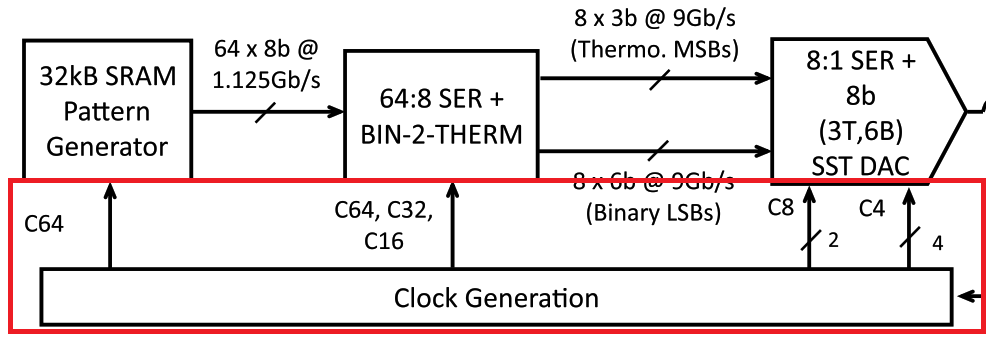
\includegraphics[width=0.8\textwidth]{System.png}
    \caption{Clock Bundle in The System.}
    \label{fig:Wire Scaling}
\end{figure}

\section{Design Challenges in High-Frequency Clock Distribution}
\label{sec:design-challenges}

At a 32 GHz operating frequency, the clock period is \textbf{31.25 ps}. This extreme speed transforms the clock distribution network from a simple routing task into a complex high-frequency design problem. The challenges are primarily driven by the physical limitations of interconnects and the active circuitry required to drive them.

\subsection{Interconnect (Wire) Scaling and Bandwidth Limits}
\label{subsec:interconnect-scaling}

As CMOS technology scales to smaller nodes, the physical properties of on-chip metal wires become the dominant bottleneck.

\begin{itemize}
    \item \textbf{RC Delay and Scaling:} Every new technology node reduces the cross-sectional area of metal traces, which causes \textbf{Resistance (R)} to increase dramatically. Simultaneously, closer proximity to other wires increases parasitic \textbf{Capacitance (C)}. The resulting RC time constant of the wire limits how fast a signal can travel. At 32 GHz, even a relatively short wire can have a delay that is a significant fraction of the total clock period.
    
    \item \textbf{The RC-LPF Effect:} High-speed interconnects behave as a \textbf{Low-Pass Filter (LPF)}. This filter attenuates high-frequency components of the signal. Because a square-wave clock relies on high-frequency harmonics to maintain its shape, the wire "rounds off" the edges. By the time a 32 GHz signal travels across the transmitter, it loses its sharp transitions, making it difficult for the Serializer to detect valid clock edges.
\end{itemize}

\begin{figure}[H]
    \centering
    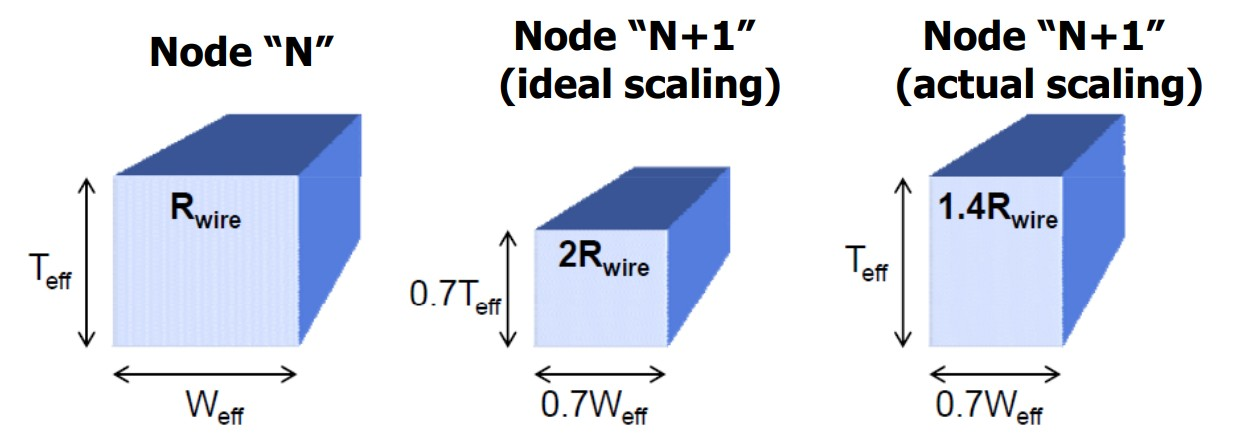
\includegraphics[width=0.7\textwidth]{Wire_scaling.jpg}
    \caption{Impact of Technology Node Scaling on Wire Resistance and Geometry.}
    \label{fig:Wire Scaling}
\end{figure}


\subsection{Cascaded Clock Buffer Chains}
\label{subsec:cascaded-buffers}

Because the 32 GHz signal is severely attenuated by the\textbf{ LPF effect} and also increased delay due to wire resistance and the large capacitive load of the Serializer, it is physically impossible to drive the signal with a single buffer stage.

\begin{itemize}
    \item \textbf{The Repeater Strategy:} To maintain a usable voltage swing over the distance from the PLL to the Serializer, a chain of cascaded buffers must be placed along the path. These buffers act as "repeaters," re-amplifying the signal at regular intervals to combat the RC losses of the interconnects.
    
    \item \textbf{Load Management:} Each buffer must be sized to drive the input capacitance of the following stage. Since the GHz Serializer presents a massive capacitive load at an extremely high frequency, the final buffers in the chain must be exceptionally large. This results in significant power consumption and silicon area penalties.
\end{itemize}

\subsection{Jitter Amplification in Buffer Chains}
\label{subsec:jitter-amplification}

A major challenge with cascaded buffers at high frequencies is \textbf{Jitter Amplification}. This occurs when the clock frequency is close to the maximum bandwidth of the buffer.

\begin{itemize}
    \item \textbf{Limited Bandwidth Effect:} At 32 GHz, the clock period is so short (31.25 ps) that the transistors in the buffer may not have enough time to reach the full supply voltage (\(V_{DD}\)) or ground before the next transition begins. When the clock frequency operates close to the buffer's cutoff frequency, the buffer acts as a low-pass filter attenuating the signal and adds Jitter.
    
    \item \textbf{Noise-to-Jitter Conversion:} The limited bandwidth results in "rounded" edges with a slow \textbf{Slew Rate}. A slow slew rate is highly dangerous because it increases the \textbf{Rise} and \textbf{Fall} time of the signal. In this region, any small voltage noise (\(\Delta V\)) on the power supply or thermal noise from the transistors is translated into a large timing displacement (\(\Delta t\)), effectively "amplifying" the jitter.
    
    \item \textbf{Cumulative Degradation:} In a cascaded chain, each stage does not just pass the jitter of the previous stage; it adds its own noise and amplifies the existing timing uncertainty. By the time the 32 GHz clock reaches the Serializer, the accumulated jitter can consume a large portion of the Unit Interval (UI), leading to a significant increase in the Bit Error Rate (BER).
\end{itemize}

\begin{figure}[H]
    \centering
    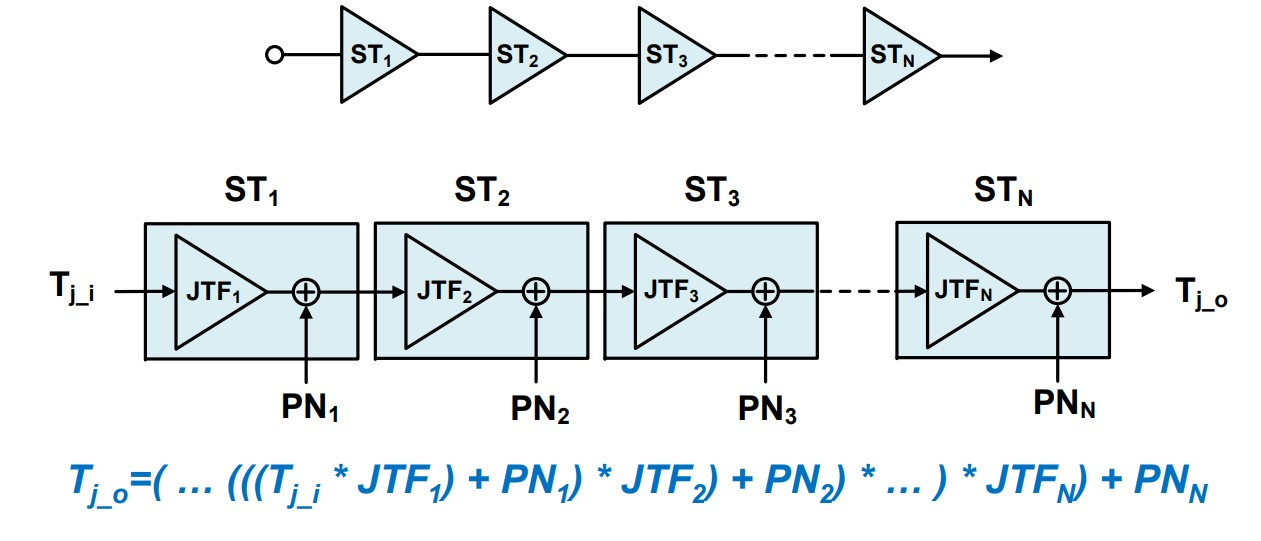
\includegraphics[width=0.8\textwidth]{buffer_chain.jpg}
    \caption{Cumulative Jitter in Cascaded Clock Buffer Chains.}
    \label{fig:Wire Scaling}
\end{figure}

\subsection{Solution: Quadrature Clocking Scheme}
\label{sec:quadrature-solution}

To overcome the severe interconnect degradation and jitter amplification at High frequencies (eg. 32 GHz), modern high-speed transmitters utilize a \textbf{Quadrature Clocking Scheme}. This approach shifts the design strategy from "Brute Force" high-frequency distribution to a more efficient multi-phase architecture.

%\subsection{Frequency Reduction (Quarter-Rate Operation)}
%\label{subsec:frequency-reduction}
\begin{itemize}
    \item\textbf{Frequency Reduction (Quarter-Rate Operation):}

The most immediate benefit of the quadrature scheme is the reduction of the distribution frequency. By using four phases—\(0^\circ, 90^\circ, 180^\circ,\) and \(270^\circ\)—the system can operate at a "Quarter-Rate." which will effectively reduce \textbf {Power consumption} and \textbf{Jitter amplification}.

\begin{itemize}
    \item \textbf{Relaxed Bandwidth:} Instead of pushing a 32 \GHz\ signal through the buffer chains, the clocking blocks deliver an 8 GHz signal.
    
    \item \textbf{Combatting the RC-LPF:} At 8 GHz, the signal is much further away from the cutoff frequency of the on-chip interconnects. This results in significantly less amplitude attenuation and preserves the sharp edges of the clock, directly addressing the "Frequency Wall" mentioned in Section \ref{subsec:interconnect-scaling}.
\end{itemize}

\begin{figure}[H]
    \centering
    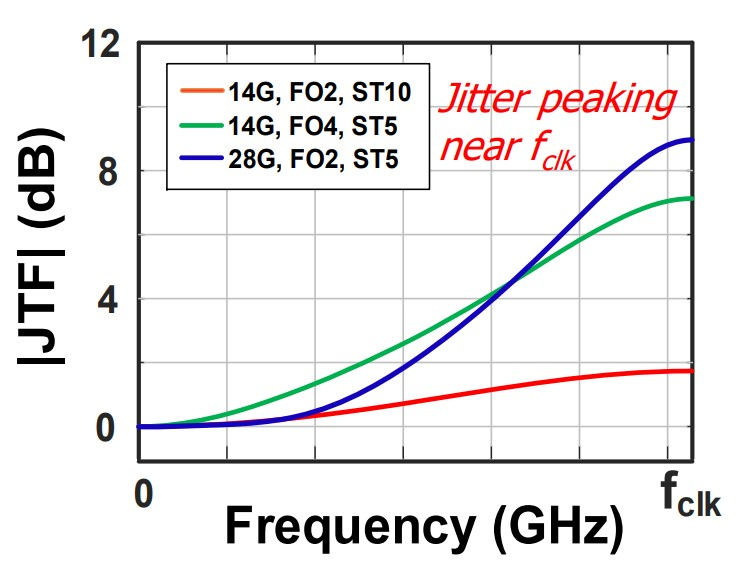
\includegraphics[width=0.8\textwidth]{Jitter_amp.jpg}
    \caption{Jitter Transfer Function (JTF(dB)) vs. Clock Frequency.}
    \label{fig:Wire Scaling}
\end{figure}

\end{itemize}


%\subsection{Maintaining Data Throughput}
%\label{subsec:maintaining-throughput}
\begin{itemize}
    \item\textbf{Maintaining Data Throughput:}

The primary challenge in moving from a 32 GHz distribution to an 8 GHz distribution is maintaining the same data rate at the output The solution is not just using four phases, but specifically shaping those phases into a \textbf{25\% duty cycle}. This serves as the direct compensation for the slower clock speed.

\subsubsection{Replicating the 32 GHz Pulse Width}
In a full-rate 32 GHz system, each bit of data has a duration (Unit Interval or UI) of exactly 31.25 ps.

\begin{itemize}
    \item If we used a standard 8 GHz clock with a 50\% duty cycle, the "High" pulse would be \textbf{62.5 ps} long—twice as long as the required bit time.
    
    \item By enforcing a \textbf{25\% duty cycle} on the 8 GHz clock (\(125 \text{ ps} \times 0.25\)), we create a pulse that is exactly \textbf{31.25 ps} wide.
\end{itemize}

In this way, the 25\% duty cycle 8 GHz clock "mimics" the timing precision of the 32 GHz clock. It provides the exact same activation window for the serializer, but at a much lower repetition rate.

\subsubsection{Phase Interleaving for Full-Rate Throughput}
Because each 8 GHz phase now only occupies 25\% of the total cycle time, we can interleave four of these phases (\(0^\circ, 90^\circ, 180^\circ, 270^\circ\)) without any overlap.

\begin{itemize}
    \item Each phase is responsible for a different "time slot" in the 32 Gbps bitstream.
    
    \item As the first phase (\(0^\circ\)) finishes its 31.25 ps pulse, the second phase (\(90^\circ\)) immediately begins its 31.25 ps pulse.
\end{itemize}

This sequential "hand-off" between the four phases ensures that the Serializer is always active, producing a continuous stream of data at 32 Gbps. This effectively \textbf{compensates} for the 4\(\times\) reduction in frequency: the clock is 4\(\times\) slower, but because we use 4 phases with 1/4th the duty cycle, the data throughput remains identical to a 32 GHz system.

\subsubsection{Benefits of Compensation}
This compensation strategy allows the transmitter to enjoy the "best of both worlds":

\begin{enumerate}
    \item \textbf{Distribution Ease:} The wires and buffers only have to handle an 8 GHz fundamental frequency, avoiding the massive attenuation and quality loss of the 32 GHz "Frequency Wall" described in Section \ref{sec:design-challenges}.
    
    \item \textbf{Timing Accuracy:} The 25\% pulse width ensures the Serializer output maintains the correct bit period (\(31.25 \text{ ps}\)), preserving the "Data Eye" width for the receiver.
\end{enumerate}

\begin{figure}[H]
    \centering
    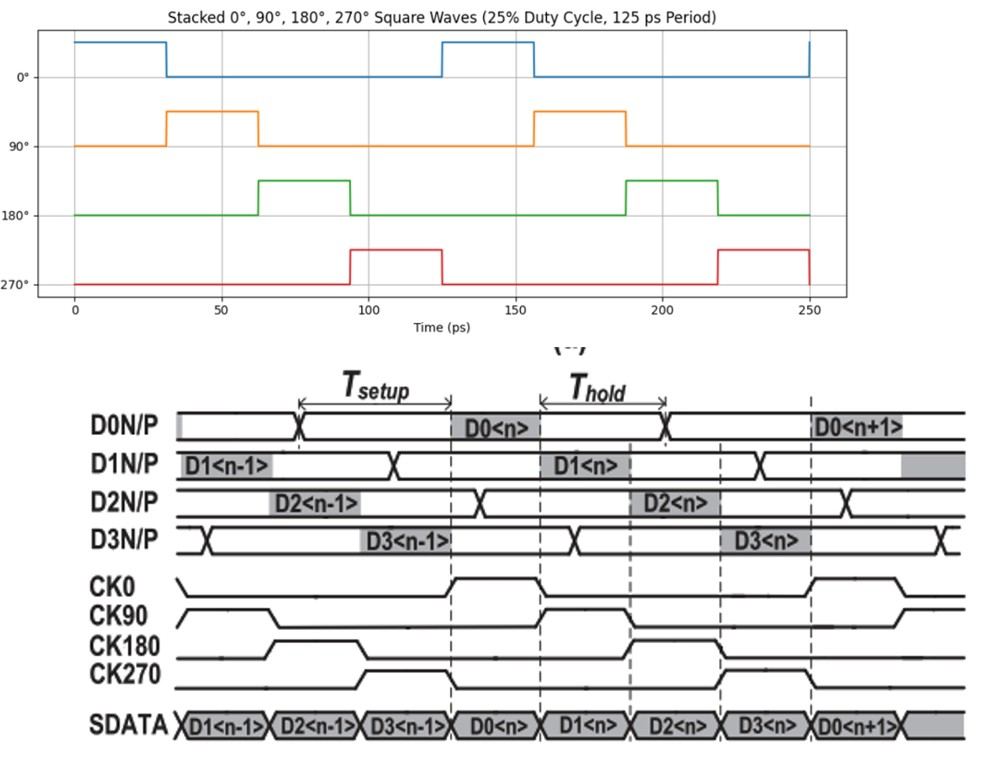
\includegraphics[width=0.8\textwidth]{quarter_rate.jpg}
    \caption{Maintaining Data Throughput using Quarter Rate Clocking Scheme.}
    \label{fig:Wire Scaling}
\end{figure}

\end{itemize}

\section{Implementation Blocks for Quadrature Clocking}
\label{sec:implementation-blocks}

To implement a robust 8 GHz quadrature scheme, the transmitter clocking path integrates a series of specialized functional blocks. These blocks transform the raw high-frequency signal from the PLL into high-integrity timing pulses required by the Serializer.

\subsection{The I/Q Frequency Divider}
\label{subsec:iq-divider}

The I/Q Divider is the primary frequency translation element and the starting point of the local clock path.

\begin{itemize}
    \item \textbf{Function:} It receives the 32 GHz high-frequency reference from the PLL and divides it down to 8 GHz.
    
    \item \textbf{Quadrature Generation:} Utilizing a master-slave latch topology, it generates the four fundamental quadrature phases (\(0^\circ, 90^\circ, 180^\circ, 270^\circ\)) at a \textbf{50\% duty cycle}.
    
    \item \textbf{Challenges:} The divider must maintain high bandwidth to ensure that Division is done with low additional  jitter while operating at the limits of the technology node.
\end{itemize}

\subsection{Pulse Shaper (25\% Duty Cycle Generator)}
\label{subsec:pulse-shaper}

Since the I/Q divider produces 50\% duty cycle phases, a dedicated \textbf{Pulse Shaper} is required to prepare the clock for the quarter-rate serializer.

\begin{itemize}
    \item \textbf{Function:} This block performs a logic operation (typically an AND of overlapping quadrature phases) to reduce the pulse width from 50\% to \textbf{25\%}.
    
    \item \textbf{Frequency Compensation:} This creates the 31.25 ps window necessary to compensate for the reduced frequency, allowing the 8 GHz clock to drive a 32 Gbps bitstream with the same precision as a 32 GHz clock.
\end{itemize}

\subsection{Duty Cycle Correction (DCC) Circuits}
\label{subsec:dcc-circuits}

The \DCC\ is a critical calibration block that maintains the integrity of the pulse width against PVT (Process, Voltage, Temperature) variations.

\begin{itemize}
    \item \textbf{50\% Correction Mode:} The DCC first ensures that the divider's outputs are perfectly symmetrical. If the 50\% duty cycle is distorted, it creates an immediate phase-shift error between the \(I\) and \(Q\) signals.
    
    \item \textbf{25\% Correction Mode:} The DCC also monitors the output of the Pulse Shaper. Because a 25\% pulse at 8 GHz is extremely narrow (31.25 ps), any drift can cause bit-width mismatch or data collisions in the Serializer. The DCC applies a correction voltage to "lock" the pulse width at exactly \(1/4\) of the clock period.
\end{itemize}

\subsection{Deskew Circuits}
\label{subsec:deskew-circuits}

The final block in the chain is the \textbf{Deskew} circuit, which provides the final "fine-tuning" of the timing edges.

\begin{itemize}
    \item \textbf{Function:} It provides independent delay control for each of the four quadrature phases.
    
    \item \textbf{Phase Orthogonality:} Even with a perfect divider, the physical metal routing to the Serializer can introduce "skew" (timing mismatches). Deskew circuits—usually digitally controlled delay lines—adjust the arrival of each phase to ensure they remain exactly \(90^\circ\) apart at the point of serialization.
    
    \item \textbf{System Impact:} This maximizes the horizontal timing margin (the "eye width") of the transmitted signal.
\end{itemize}

\subsection{Summary of Service}
\label{subsec:summary-service}

The I/Q Divider provides the raw phases, but open-loop division is susceptible to PVT (Process, Voltage, Temperature) variations. By including \textbf{DCC and Deskew circuits}, we create a robust clocking path that can calibrate itself to maintain 90\(^\circ\) precision and 50\% duty cycle regardless of manufacturing mismatches. This directly leads to a wider 'Data Eye' and a lower Bit Error Rate (BER) at the transmitter output.


\begin{table}[ht]
    \centering
    \caption{Quadrature Clocking Path Functional Blocks Summary}
    \label{tab:clocking-blocks}
    \begin{adjustbox}{width=\textwidth}
    \begin{tabular}{lcccc}
        \toprule
        \textbf{Block} & \textbf{Input Frequency} & \textbf{Output Frequency} & \textbf{Duty Cycle Focus} & \textbf{Primary Purpose} \\
        \midrule
        \textbf{I/Q Divider} & 16 \GHz & \textbf{8 \GHz} & 50\% & Frequency reduction \& \(I/Q\) generation \\
        \textbf{Pulse Shaper} & 8 \GHz & \textbf{8 \GHz} & 25\% & Frequency compensation (31.25 ps pulse) \\
        \textbf{DCC} & 8 \GHz & \textbf{8 \GHz} & 50\% \& 25\% & Preventing Duty Cycle Distortion (\DCD) \\
        \textbf{Deskew} & 8 \GHz & \textbf{8 \GHz} & Phase Alignment & Correcting routing-induced phase skew \\
        \bottomrule
    \end{tabular}
    \end{adjustbox}
\end{table}

\section{Jitter in High-Speed Clocking}
\label{sec:jitter-analysis}

Following the hardware implementation, it is essential to analyze the timing uncertainty, or jitter, that these blocks introduce. At 32 Gbps, jitter management is the primary factor in determining the system's reliability.

\subsection{Eye Diagram and Specification Mask}
\label{subsec:eye-diagram}

For proper operation, high-speed links must maintain margin in both the voltage and timing domains.

\begin{itemize}
    \item \textbf{Interoperability:} To allow independent design of the transmitter (TX) and receiver (RX), a "spec eye mask" is used, which is determined by the specific industry standard (e.g., PCIe, Ethernet).
    
    \item \textbf{Performance Guarantee:} The signal must not violate this mask to guarantee a minimum level of performance.
\end{itemize}

\begin{figure}[H]
    \centering
    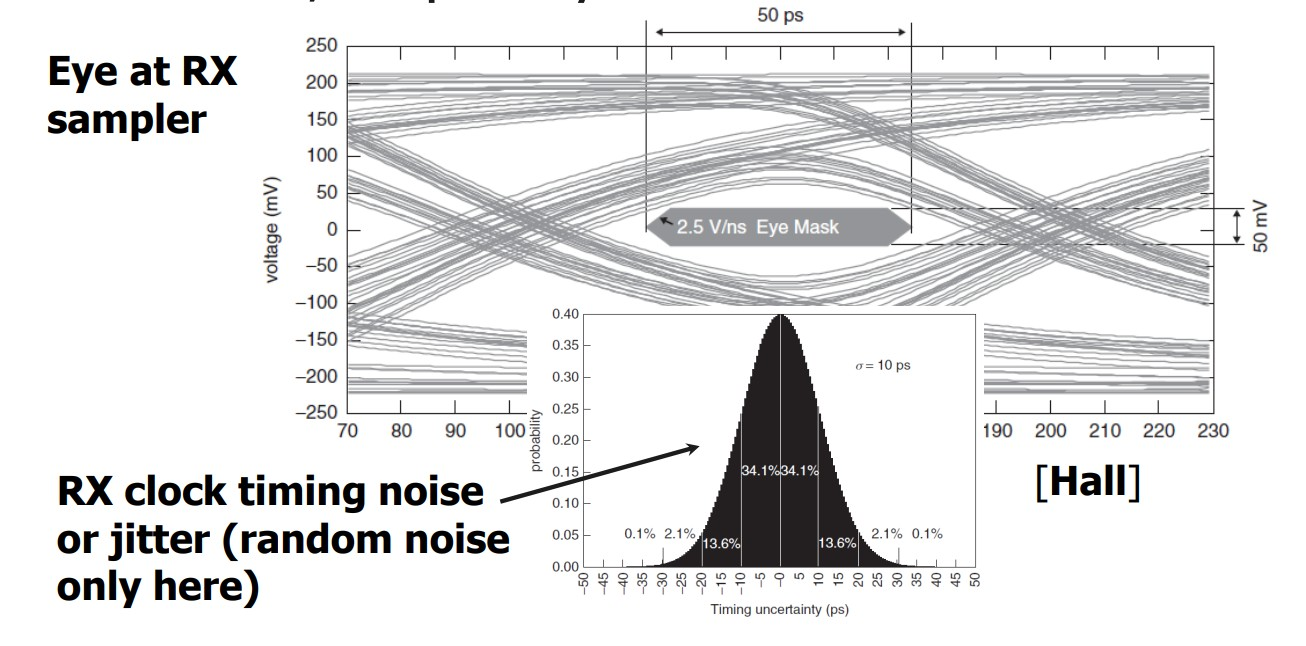
\includegraphics[width=0.8\textwidth]{Eye_mask.jpg}
    \caption{Spec Mask.}
    \label{fig:Wire Scaling}
\end{figure}


\subsection{Jitter Definitions and Measurements}
\label{subsec:jitter-definitions}

Based on how we observe the signal, jitter is categorized into three measurement types:

\begin{itemize}
    \item \textbf{Period Jitter (\(J_{\text{PER}}\)):} The deviation of a single clock period from the ideal period (\(T_{\text{ideal}}\)). It is the most basic measure of clock stability.
    
    \item \textbf{Cycle-to-Cycle Jitter (\(J_{\text{CC}}\)):} The difference in duration between two consecutive clock periods. Important for budgeting on-chip digital circuits cycle time.
    
    \item \textbf{Accumulated Jitter (\(J_{\text{AC}}\)):} Also known as Long-Term Jitter, it measures the displacement of a clock edge relative to an ideal trigger after \(N\) cycles. This is the most critical metric for our transmitter, as it defines how much the clock drifts over the time required for serialization.
\end{itemize}

\begin{figure}[H]
    \centering
    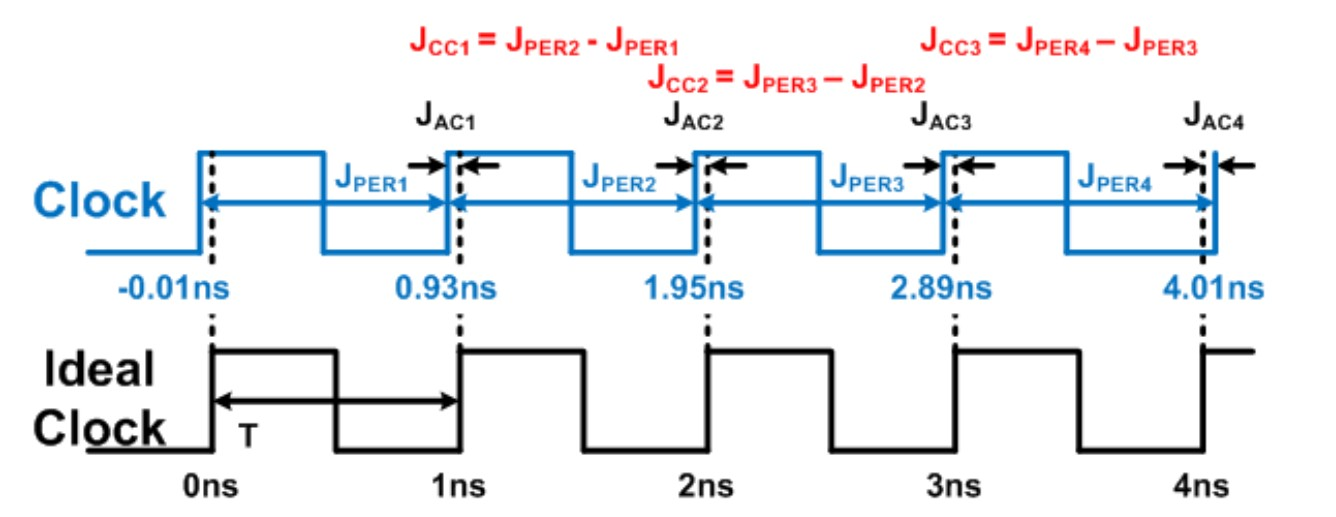
\includegraphics[width=0.8\textwidth]{jitter_param.jpg}
    \caption{Jitter Definitions.}
    \label{fig:Wire Scaling}
\end{figure}

\subsection{Jitter Statistical Parameters}
\label{subsec:statistical-parameters}

Since jitter is a stochastic (random) process, we describe it using statistical metrics:

\begin{itemize}

\item \textbf{Mean Value:}
    Can be interpreted as a fixed timing offset or “skew”, Generally not important, as usually can corrected for.



    \item \textbf{RMS Jitter (\(\sigma\)):} The standard deviation of the jitter distribution. It is used to describe Random Jitter (\(\RJ\)).
    
    \item \textbf{Peak-to-Peak Jitter (\(J_{\text{PP}}\)):} Function of both deterministic (bounded) and random
    (unbounded) jitter components, Must be quoted at a given BER to account for random
    (unbounded) jitter.
    
\end{itemize}

\subsection{Detailed Classification of Jitter Components}
\label{subsec:jitter-classification}

Total Jitter (\(\TJ\)) is the result of various independent, correlated and uncorrelated noise sources. To manage a 64 Gbps link, we must categorize these components based on their statistical properties.

\subsubsection{Random Jitter (\(\RJ\))}
Random Jitter is timing noise that is unpredictable and follows a stochastic process.

\begin{itemize}
    \item \textbf{Sources \& Causes:}
    \begin{itemize}
        \item \textbf{Thermal Noise:} Generated by the random motion of electrons in conductors and transistors. It increases with temperature.
        \item \textbf{Flicker Noise (\(1/f\)):} Low-frequency noise caused by "traps" at the silicon-dielectric interface.
    \end{itemize}
    
    \item \textbf{Characteristics:}
    \begin{itemize}
        \item\ \textbf{unbounded}, follows a \textbf{Gaussian (Normal) Distribution} 
        \item\ Assumed to have zero mean value.
        \item\  It is quantified by its RMS value (\(\sigma\)).
    \end{itemize}
\end{itemize}

\begin{equation}
    \centering
    RJ(t) = \frac{1}{\sqrt{2\pi}\sigma_{RJ}} e^{\frac{-t^2}{2\sigma_{RJ}^2}}
\end{equation}

\begin{figure}[H]
    \centering
    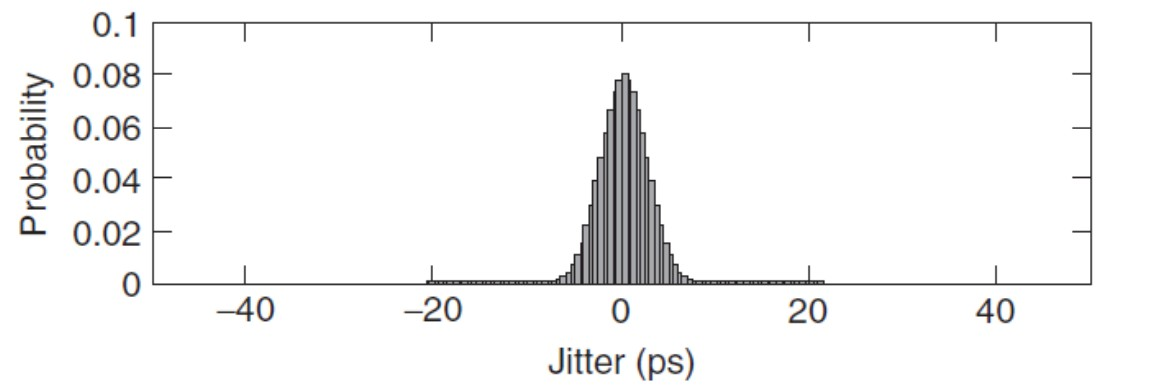
\includegraphics[width=0.8\textwidth]{RJ.jpg}
    \caption{Probability Density Function (PDF) of Random Jitter.}
    \label{fig:Wire Scaling}
\end{figure}

\subsubsection{Deterministic Jitter (\(\DJ\))}
Deterministic Jitter is bounded; it has a specific maximum peak-to-peak value.
\begin{itemize}
    \item \textbf{causes:}
    \begin{itemize}
    \item \ Transmission-line losses (ISI)
    \item\ Duty Cycle Distortion (DCD)
    \item\ Spread Spectrum Clocking
    \item\ Crosstalk
    \end{itemize}
\end{itemize}

\begin{figure}[H]
    \centering
    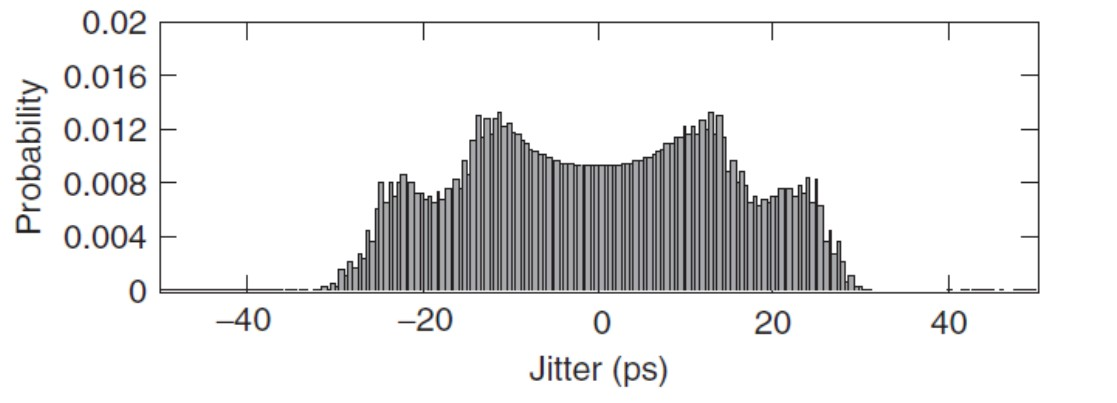
\includegraphics[width=0.8\textwidth]{DJ.jpg}
    \caption{Probability Density Function (PDF) of Determinstic Jitter.}
    \label{fig:Wire Scaling}
\end{figure}

\subsubsection{Sinusoidal or Periodic Jitter (SJ or PJ):} 
Repeats at a fixed frequency due to modulating effects.

\begin{itemize}
    \item \textbf{Spread spectrum clocking:}
    \item \textbf{PLL reference clock feedthrough:}
\end{itemize}

\begin{equation}
    \centering
    PDF_{SJ}(t) = 
    \begin{cases} 
      \frac{1}{\pi\sqrt{A^2 - t^2}} & A > |t| \\
      0 & A \leq |t| 
    \end{cases}
\end{equation}

\begin{figure}[H]
    \centering
    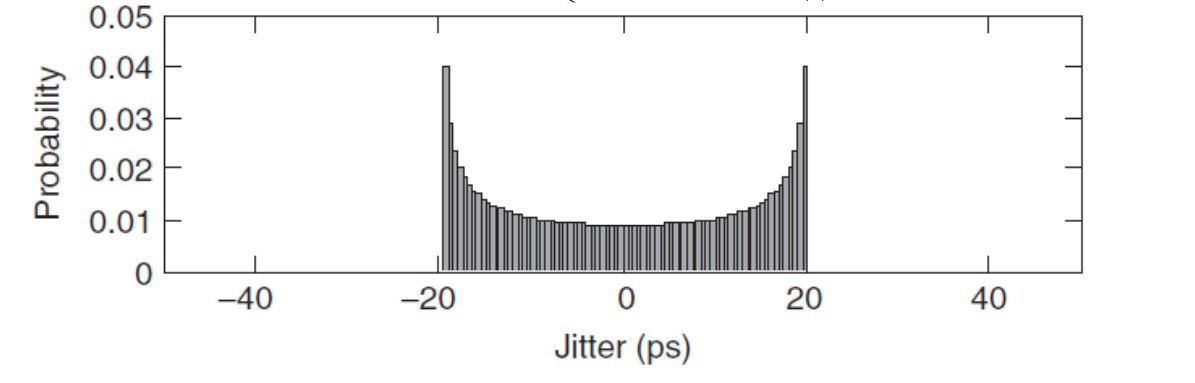
\includegraphics[width=0.8\textwidth]{SJ.jpg}
    \caption{Probability Desity Function (PDF) of Sinusoidal Jitter.}
    \label{fig:Wire Scaling}
\end{figure}

\subsubsection{Data-Dependent Jitter (DDJ):}
    Data dependent jitter is correlated with either the transmitted data pattern or aggressor (crosstalk).

\begin{itemize}
    \item \textbf{Intersymbol Interference (ISI):}
    \begin{itemize}
        \item \textbf{Source:} Caused by channel loss, dispersion, and reflections.
        \item \textbf{Cause:} As discussed in the 32 GHz challenges, the RC-LPF effect prevents the signal from reaching full rail-to-rail swing before the next transition. The "memory" of previous bits shifts the threshold crossing point of the current bit.
        \item Can be improved by equalitzation.

\begin{figure}[H]
    \centering
    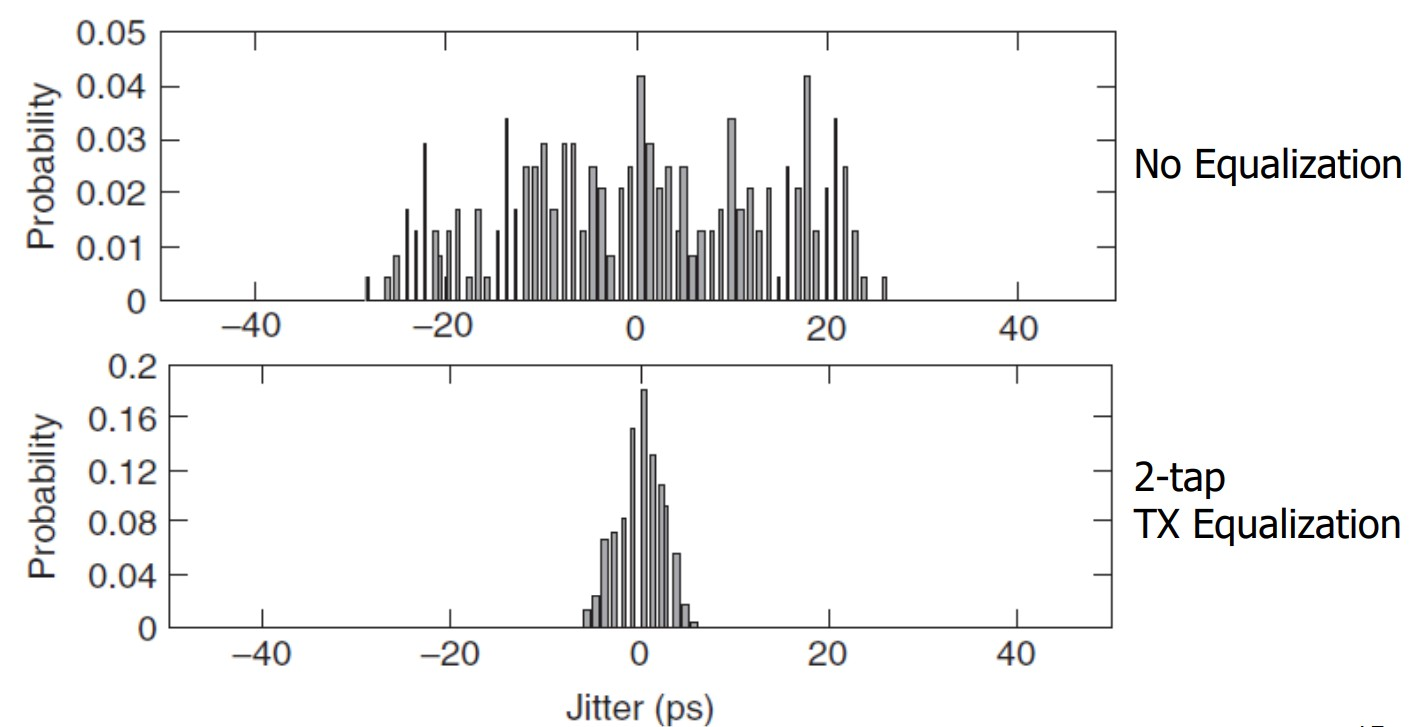
\includegraphics[width=0.8\textwidth]{ISI.jpg}
    \caption{Probability Density Function (PDF) Of Inter-Symbol Interference Jitter.}
    \label{fig:Wire Scaling}
\end{figure}
        
    \end{itemize}
\end{itemize}

\begin{itemize}
    \item \textbf{Duty Cycle Distortion (DCD):}
    \begin{itemize}
        \item \textbf{Source:} Caused by duty cycle errors in TX serialization clocks and rise/fall delay mismatches.
        \end{itemize}
       \begin{itemize}
        \item \textbf{Rise/Fall Time Mismatch:} The buffers driving the output often have different slew rates for rising and falling edges. This is primarily caused by unequal strengths (W/L ratios) or switching speeds between PMOS and NMOS transistors.
        \item \textbf{Voltage Offsets:} DC offsets in the differential signals of the I/Q divider, often due to process variations or threshold voltage (\(V_{\text{th}}\)) mismatches, cause the signal to cross the switching threshold earlier or later than intended.
    \end{itemize}
    \item \textbf{Effect:}
    \begin{itemize}
        \item \textbf{Window Shrinkage:} DCD deviates the clock from the ideal 50\% or 25\% duty cycle. This results in the "sampling" windows for the four quadrature phases being unequal in width.
        \item \textbf{Bit-Width Mismatch:} One bit in the 32 Gbps stream becomes wider while the next becomes narrower. This "non-ideal zero-crossing" reduces the horizontal timing margin (eye-width), making the system highly sensitive to error at the Serializer output.
    \end{itemize}
\end{itemize}


\begin{equation}
    \centering
    PDF_{DCD}(t) = \frac{1}{2} \left[ \delta\left(t - \frac{\alpha_{DCD}}{2}\right) + \delta\left(t + \frac{\alpha_{DCD}}{2}\right) \right]
\end{equation}

\begin{figure}[H]
    \centering
    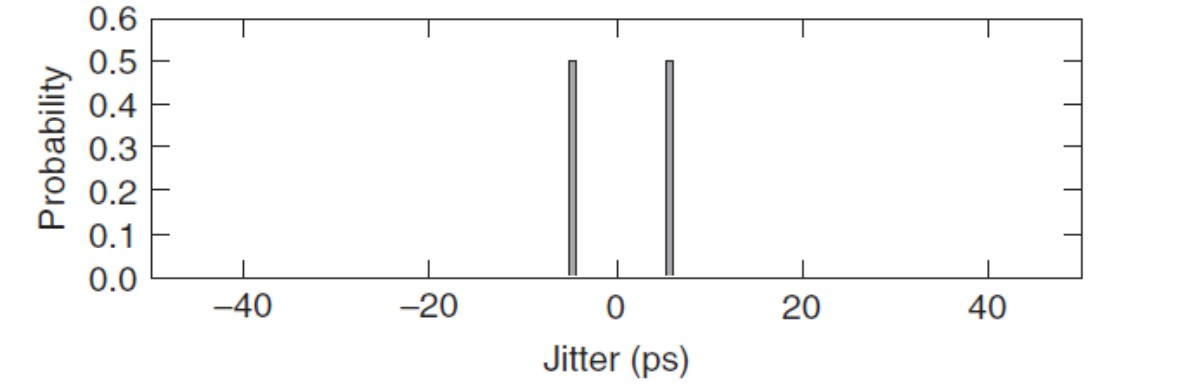
\includegraphics[width=0.8\textwidth]{DCD.jpg}
    \caption{Probability Desity Function (PDF) of Duty Cycle Distortion Jitter.}
    \label{fig:Wire Scaling}
\end{figure}


\begin{itemize}
\item \textbf{Bounded Uncorrelated Jitter (BUJ):}


\begin{itemize}
    \item \textbf{Source:} Primarily \textbf{Crosstalk}.
    \item \textbf{Cause:} When a nearby high-speed signal (aggressor) switches, it injects a current spike into the clock line (victim) via mutual capacitance or inductance.
    \item \textbf{Characteristics:} It is "Uncorrelated" because the aggressor's data usually has no relationship with the clock, but it is "Bounded" because the interference has a maximum physical limit.
    \end{itemize}
\end{itemize}


\subsection{Total Jitter (TJ)}
The total jitter PDF is produced by convolving the random and deterministic jitter PDFs.
The Total Jitter (TJ) represents the overall timing uncertainty in the system. The probability density function (PDF) of total jitter is mathematically derived by convolving the individual PDFs of random and deterministic jitter components:

\begin{equation}
    PDF_{JT}(t) = PDF_{RJ}(t) * PDF_{DJ}(t)
\end{equation}

where the deterministic jitter PDF is itself a result of the convolution of several sub-components, including Periodic (Sinusoidal) Jitter ($SJ$), Duty Cycle Distortion ($DCD$), Intersymbol Interference ($ISI$), and Bounded Uncorrelated Jitter ($BUJ$):

\begin{equation}
    PDF_{DJ}(t) = PDF_{SJ}(t) * PDF_{DCD}(t) * PDF_{ISI}(t) * PDF_{BUJ}(t)
\end{equation}

\begin{figure}[H]
    \centering
    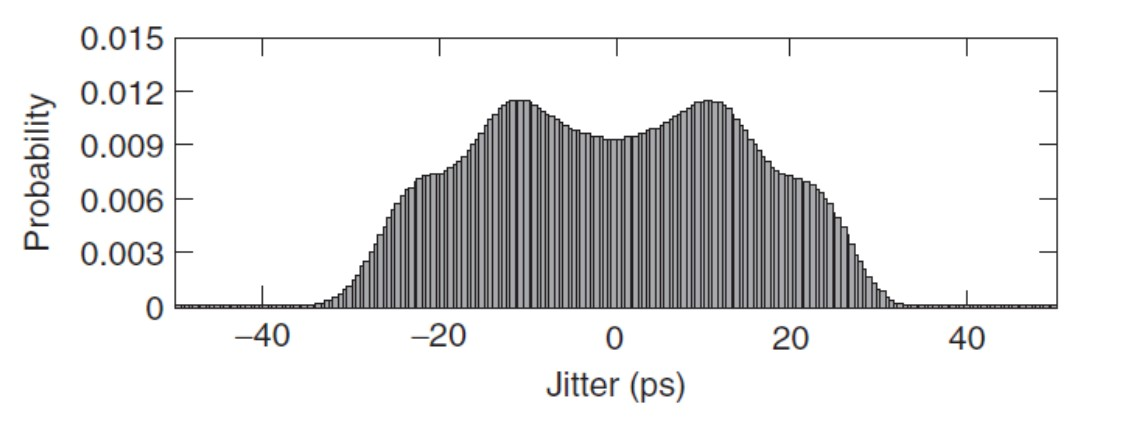
\includegraphics[width=0.8\textwidth]{TJ.jpg}
    \caption{Probability Desnity Function (PDF) of Total Jitter .}
    \label{fig:Wire Scaling}
\end{figure}


\subsection{System Jitter Budgeting}
\label{subsec:jitter-budgeting}

Jitter budgeting is the mathematical process used to ensure that the cumulative timing uncertainty from all sources—transmitter, clock distribution, and channel—does not exceed the Unit Interval (UI). To guarantee a specific Bit Error Rate (BER), jitter components must be combined according to their statistical nature.

\subsubsection{Linear Addition of Deterministic Jitter (\(\DJ\))}
Deterministic Jitter components are bounded and have fixed peak-to-peak values. The convolution of multiple bounded jitter distributions is approximated by the linear sum of their individual peak-to-peak terms:

\begin{equation}
    D_{J,\text{total}} = \sum D_{J,i} = D_{J,\text{ISI}} + D_{J,\text{DCD}} + D_{J,\text{Pj}} + \cdots
\end{equation}

Since \(\DJ\) is not random, every pico second of deterministic jitter added to the system directly reduces the available timing window for sampling.

\subsubsection{Root-Sum-Square (RSS) of Random Jitter (\(\RJ\))}
Random jitter sources (such as thermal and shot noise) are uncorrelated and follow a Gaussian distribution. To calculate the total system \(\RJ\), the RMS values are combined using the RSS method:

\begin{equation}
    \sigma_{\RJ,\text{total}} = \sqrt{\sigma_{\RJ,1}^2 + \sigma_{\RJ,2}^2 + \sigma_{\RJ,3}^2 + \cdots}
\end{equation}

This statistical approach is used because it is highly improbable for multiple independent random noise sources to reach their peak displacement simultaneously.

\subsubsection{Total Jitter (TJ) and the Dual-Dirac Model}
The Dual-Dirac model is the industry standard for predicting eye closure at a specific BER. It combines the bounded \(\DJ\) and the unbounded Gaussian \(\RJ\):

\begin{equation}
    T_J(\text{BER}) = D_{J,pp} + Q(\text{BER}) \cdot \sigma_{R_J,total}
\end{equation}

\begin{itemize}
    \item \textbf{The Q-Factor:} This multiplier represents the number of standard deviations required to achieve a target probability on the Gaussian tails.
    
    \item \textbf{The \(14\sigma\) Rule:} For a common target of BER = \(10^{-12}\), the \(Q\) factor is approximately 14 (representing \(7\sigma\) on each side of the transition). In this case, the equation becomes:
    \end{itemize}
    
   \begin{equation}
    T_J = D_{J,pp} + 14 \cdot \sigma_{R_J,total}
\end{equation}

\subsubsection{The Timing Margin Requirement}
A high-speed link is considered functional only if the Total Jitter is less than the Unit Interval, leaving sufficient margin for the receiver:

\begin{equation}
    \UI \geq \TJ(\BER) + \text{Receiver Margin}
\end{equation}

If the total jitter exceeds the UI, the "Data Eye" closes, and the receiver will be unable to distinguish between bit transitions, leading to a failure to meet the BER target. Design techniques such as Duty Cycle Correction (DCC) and Deskewing are employed specifically to reclaim this timing margin by minimizing the \(\DJ\) components.

\begin{figure}[H]
    \centering
    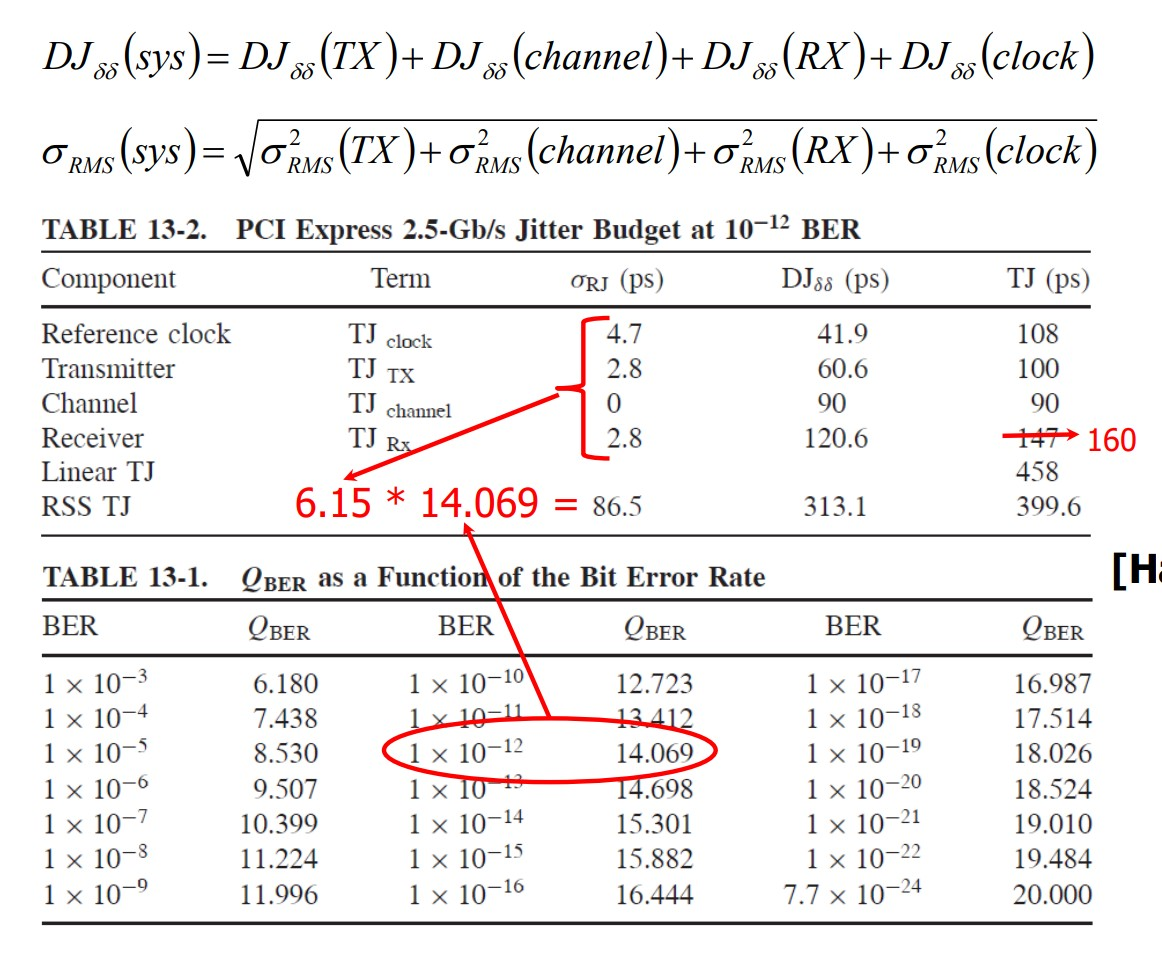
\includegraphics[width=0.8\textwidth]{Jitter_ex.jpg}
    \caption{Jitter budgeting Example.}
    \label{fig:Wire Scaling}
\end{figure}




\section{Fundamentals of High-Speed Serialization}
The core function of a high-speed transmitter is to convert parallel low-speed data from the digital core into a serial high-speed stream suitable for transmission over the physical medium. This Parallel-In Serial-Out (PISO) operation is the final and most critical stage of the digital-to-analog interface. As data rates scale towards 64 Gb/s and beyond, the serializer (Multiplexer or Mux) becomes the primary bandwidth bottleneck. This chapter reviews the fundamental serialization architectures and presents a literature survey of circuit topologies used to implement the high-speed multiplexer.

\subsection{The Parallel-In Serial-Out (PISO) Concept}
A PISO block receives $N$ parallel data streams, each running at a frequency of $f_{clk}/N$, and interleaves them into a single serial stream running at the full baud rate $f_{baud}$. In the context of PAM4 signaling, the serializer operates on symbols rather than individual bits. For a 64 Gb/s PAM4 link, the symbol rate is 32 Gbaud.

The design of the PISO stage is governed by the trade-off between the complexity of the clock distribution network and the switching speed of the multiplexing circuits.

\begin{figure}[H]
    \centering
    % REPLACE 'piso.jpg' with your filename
    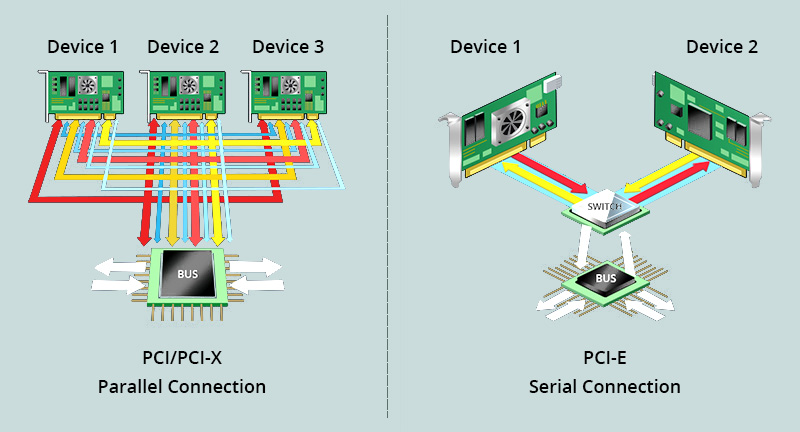
\includegraphics[width=0.8\textwidth]{piso.jpg}
    \caption{Conceptual operation of the Parallel-In Serial-Out (PISO) block: Converting parallel low-speed data streams into a single high-speed serial output.}
    \label{fig:piso_diagram}
\end{figure}

\subsection{Serialization Rate Architectures}
To achieve a target symbol rate of 32 Gbaud (for 64 Gb/s PAM4), three primary clocking architectures are typically discussed in literature: Full-Rate, Half-Rate, and Quarter-Rate.

\subsubsection{Full-Rate Architecture}
In a Full-Rate architecture, the serializer is driven by a clock frequency equal to the output symbol rate. For a 32 Gbaud link, this requires a 32 GHz clock signal.

\begin{itemize}
    \item \textbf{Operation:} The circuit retimes the data on every rising edge of the clock, requiring the latching elements to operate at the fundamental frequency of the data stream.
    \item \textbf{Limitations:} The primary bottleneck of this topology is the stringent timing budget. The entire serialization operation—including the clock-to-output delay ($t_{c-q}$) and the setup time ($t_{setup}$)—must complete within a single Unit Interval (UI). As data rates scale, the UI shrinks (e.g., only 31.25 ps at 32 Gbaud), leaving vanishingly small margins for process variations or jitter.
\end{itemize}

\subsubsection{Half-Rate Architecture}
Half-Rate architectures utilize a clock frequency at half the baud rate (16 GHz for 32 Gbaud).
\begin{itemize}
    \item \textbf{Operation:} Data is sampled on both the rising and falling edges of the clock (Double Data Rate or DDR). This effectively acts as a 2:1 multiplexer in the final stage.
    \item \textbf{Limitations:} While it relaxes the clock frequency, Half-Rate architectures are highly sensitive to Duty Cycle Distortion (DCD). If the clock duty cycle deviates from exactly 50\%, the ``even'' symbols will have a different width than the ``odd'' symbols, directly closing the eye diagram horizontally.
\end{itemize}

\subsubsection{Quarter-Rate Architecture}

Quarter-Rate architectures utilize a clock frequency at one-quarter of the baud rate (e.g., 8 GHz for 32 Gbaud). This approach further relaxes the timing constraints on the latching elements but increases the complexity of the clock generation and distribution network.

\begin{itemize}
    \item \textbf{Operation:} The serializer functions as a 4:1 multiplexer, combining four parallel low-speed data streams into a single high-speed output. This requires four clock phases spaced 90$^{\circ}$ apart ($\Phi_0, \Phi_{90}, \Phi_{180}, \Phi_{270}$) to sequentially select the input bits.

    \item \textbf{Duty Cycle Selection:} A critical design distinction in Quarter-Rate topologies is the choice between 50\% and 25\% clock duty cycles.
    \begin{itemize}
        \item \textit{50\% Duty Cycle:} Standard quadrature clocks naturally have a 50\% duty cycle, meaning each phase is active for 2 Unit Intervals (UI). Since the target bit period is 1 UI, adjacent clock phases inherently overlap. Using these directly would cause signal contention (short circuits) at the multiplexer output.
        \item \textit{25\% Duty Cycle (Selected):} To eliminate contention, this implementation utilizes a \textbf{25\% duty cycle} scheme. By reducing the pulse width to exactly 1 UI, the four clock phases become strictly non-overlapping. This ensures that only one slice drives the output at any given instant, allowing for robust serialization without the need for additional gating logic.
    \end{itemize}
\end{itemize}
\begin{figure}[H]
    \centering
    % REPLACE 'piso.jpg' with your filename
    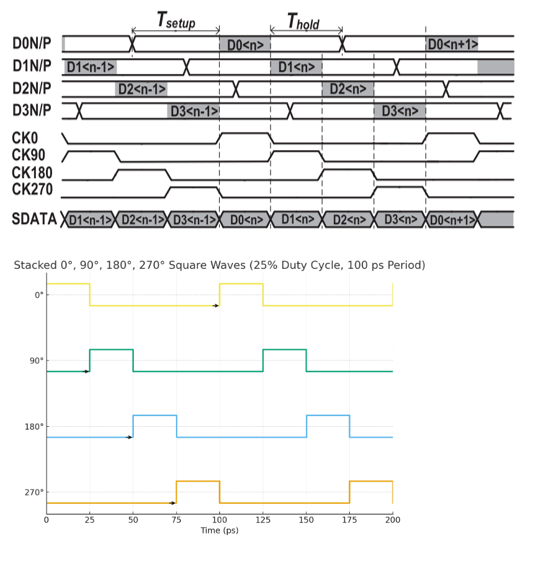
\includegraphics[width=0.8\textwidth]{core idea.png}
    \caption{Timing diagram of the Quarter-Rate serialization scheme. The lower waveforms depict the proposed 25\% duty cycle clock phases ($0^\circ, 90^\circ, 180^\circ, 270^\circ$), which create strictly non-overlapping selection windows to sequentially serialize the parallel input data ($D_0-D_3$) without signal contention.}
    \label{fig:quarter_rate_timing}
\end{figure}

% =========================================================
% REVISED LITERATURE REVIEW (Neutral & Professional)
% =========================================================
\section{Literature Review of Multiplexer Topologies}
\label{sec:lit_review}

The design of the final 4:1 multiplexer stage is critical for signal integrity. Over the past decade, three primary circuit topologies have dominated the literature for high-speed serialization: Transmission Gates (TG), Current-Mode Logic (CML), and CMOS Tri-State Logic. This section surveys their operating principles and performance trade-offs in the context of high-speed PAM4 signaling.

\subsection{Passive Transmission Gate (TG) based Topology}
The CMOS Transmission Gate (TG) functions as a high-speed passive switch, utilizing parallel NMOS and PMOS devices to pass the signal from input to output.

\begin{figure}[H]
    \centering
    % REPLACE 'piso.jpg' with your filename
    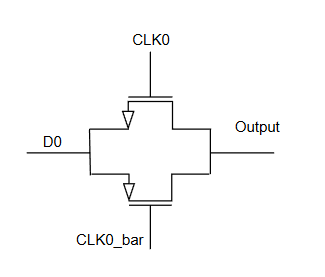
\includegraphics[width=0.5\textwidth]{tg.png}
    \caption{Simple Schematic diagram of a CMOS Transmission Gate (TG) switch used in high-speed multiplexers.}
    \label{fig:tg_schematic}
\end{figure}

\begin{itemize}
    \item \textbf{Advantages:} The primary appeal of the TG topology is its zero static power consumption. Since it contains no direct path from supply to ground, it is theoretically the most power-efficient architecture for low-frequency applications.
    \item \textbf{Limitations:} As reviewed in recent literature, TG-based muxes face severe challenges at high data rates . The "Self-Loading" effect becomes dominant: to reduce the on-resistance ($R_{on}$), the transistor width must be increased, which inevitably increases the parasitic capacitance ($C_{par}$). This creates a fundamental bandwidth limit.also 
\end{itemize}

\subsection{Current-Mode Logic (CML) based Topology}
Current-Mode Logic (CML) relies on steering a constant tail current between differential branches to generate the output voltage.
\begin{figure}[H]
    \centering
    % REPLACE 'piso.jpg' with your filename
    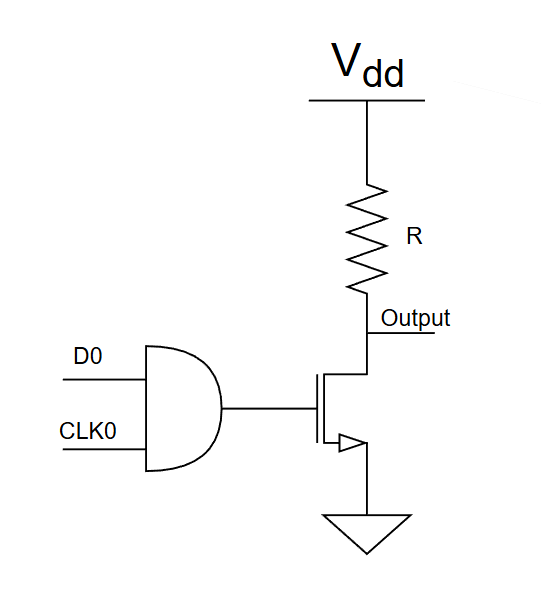
\includegraphics[width=0.5\textwidth]{cml slice.png}
    \caption{Schematic of a Current-Mode Logic (CML) driver stage with a resistive load. In this implementation, the data ($D_0$) is logically combined with the clock ($CLK_0$) to gate the NMOS driver, steering current through the load resistor $R$ only during the active phase.}
    \label{fig:cml_schematic}
\end{figure}
\begin{itemize}
    \item \textbf{Advantages:} CML is widely regarded in literature as the fastest logic family. Its differential nature provides excellent common-mode noise rejection, and its low voltage swing enables extremely fast switching speeds, making it a standard choice for optical and 100G+ interfaces.
    \item \textbf{Limitations:} The major drawback of CML is its high static power consumption, which occurs even when the data is not switching. Furthermore, the output swing is limited by the $I_{tail} \times R_{load}$ product. Achieving a high swing for acceptable SNR requires a large tail current or large load resistors, both of which degrade the power-bandwidth trade-off.
\end{itemize}

\subsection{Active Tri-State Inverter based Topology}
The Tri-State inverter topology utilizes a clocked inverter structure (a stack of series transistors) to actively drive the output node.
\begin{figure}[H]
    \centering
    % Keeping the size consistent with the CML figure
    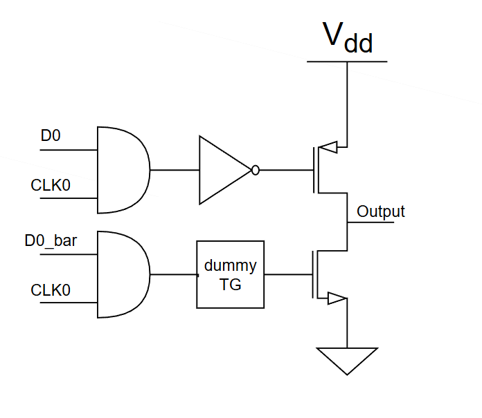
\includegraphics[width=0.5\textwidth]{tri_slice.png}
    
    \caption{Schematic implementation of the Active Tri-State Inverter branch. The data inputs ($D_0$ and $\overline{D_0}$) are logically AND-ed with the clock phase ($CLK_0$). This ensures that both the PMOS and NMOS transistors are turned OFF (High-Impedance state) when the clock is inactive, preventing contention with other branches.}
    \label{fig:tristate_schematic_implementation}
\end{figure}

\begin{itemize}
    \item \textbf{Advantages:} Unlike the passive TG, the Tri-State topology is "active," meaning it regenerates the signal levels. This allows for a full rail-to-rail voltage swing, which maximizes the vertical eye opening and Signal-to-Noise Ratio (SNR).
    \item \textbf{Limitations:} The primary challenge documented in literature is Dynamic Power consumption. Since power scales with $CV^2f$, driving a full-swing signal at 64 Gb/s results in significant dynamic energy dissipation. Additionally, this topology is susceptible to "shoot-through" current (short-circuit power) during the brief moments when both PMOS and NMOS networks are partially on, requiring precise timing control of the clock phases.
\end{itemize}

% =========================================================
% SECTION 2.3: SELECTION & ANALYSIS
% =========================================================
\section{Architecture Selection and Comparative Analysis}
\label{sec:arch_selection}

Following the review of available topologies, this section presents a comparative analysis based on the critical metrics for a 64 Gb/s PAM4 transmitter: Bandwidth, Power Consumption, jitter and Output Swing.

\subsection{Comparative Performance Metrics}
Table \ref{tab:topology_comparison} summarizes the trade-offs between the Transmission Gate (TG), Current-Mode Logic (CML), and Active Tri-State Inverter topologies based on recent literature in 22nm and similar nodes.

\begin{table}[htbp]
    \centering
    \caption{Comparative Analysis of Multiplexer Topologies for High-Speed SerDes}
    \label{tab:topology_comparison}
    \renewcommand{\arraystretch}{1.3} % Adds spacing to rows
    
    % The \resizebox command forces the table to fit exactly in the text width
    \resizebox{\textwidth}{!}{%
        \begin{tabular}{|l|c|c|c|}
        \hline
        \textbf{Metric} & \textbf{Transmission Gate (TG)} & \textbf{Current-Mode Logic (CML)} & \textbf{Tri-State Inverter} \\ \hline
        \textbf{Bandwidth} & Low  & Very High & High \\ \hline
        \textbf{Static Power} & Zero (Leakage only) & High (Constant Tail Current) & Zero (Leakage only) \\ \hline
        \textbf{Dynamic Power} & Low & Low & High ($CV^2f$) \\ \hline
        \textbf{Output Swing} & Rail-to-Rail ($V_{DD}$) & Limited ($I \times R$) & Rail-to-Rail ($V_{DD}$) \\ \hline
        \textbf{Design Complexity} & Simple & High) & Moderate (Timing critical) \\ \hline
        \end{tabular}%
    }
\end{table}

\subsection{Critical Analysis for PAM4 Applications}
For PAM4 signaling, Linearity and Signal-to-Noise Ratio (SNR) are paramount.

\begin{enumerate}
    \item \textbf{Bandwidth vs. Power:} While CML offers the highest raw bandwidth, the static power required to drive a low-impedance load at 64 Gb/s is prohibitive for energy-efficient designs. Conversely, the TG topology cannot support the required bandwidth due to the self-loading effect discussed in Section \ref{sec:lit_review}.
    
    \item \textbf{Voltage Swing and SNR:} PAM4 signals have three eyes, meaning the vertical eye opening is $1/3$ that of NRZ. Maximizing the output voltage swing is critical to maintaining a sufficient SNR. 
    \begin{itemize}
        \item CML topologies typically provide a reduced swing, which degrades the SNR.
        \item The Tri-State and TG topologies offer a full rail-to-rail swing ($0$ to $0.8$ V in 22nm FD-SOI), providing the maximum possible vertical eye opening without needing additional amplification stages.
    \end{itemize}
\end{enumerate}

%%%%%%%%%%%  DRIVER  %%%%%%%%%%%%%%%%%%%%%%%%%%%
\section{The Function of the Driver} \label{sec:driver_function}
The most challenging building block in TX design is typically the line driver as it faces the most difficult demands of the standard: it must deliver high current levels to the channel while meeting the bandwidth requirements and maintaining signal integrity.

\subsection{Signal Integrity} \label{subsec:signal_integrity}
A driver with good signal integrity must successfully generate a signal with:

\begin{tasks}[label=$\bullet$, column-sep=10pt](2) % The (2) creates two columns
    \task High bit rate
    \task Low power consumption
    \task Low noise
    \task Free of unnecessary time domain spikes
    \task Precise $50\,\Omega$ impedance matching to prevent reflections
    \task High linearity to maintain uniform PAM-4 eye levels (RLM)
    \task Compensation for channel-induced Inter-Symbol Interference (ISI) through equalization
\end{tasks}
A useful visualization of signal integrity is the \textbf{eye diagram}
\subsection{Termination} \label{subsec:termination}
\begin{itemize}
    \item \textbf{Poly resistors} are typically used due to better linearity, but they typically vary $\pm 30\%$ over process and temperature. To mitigate this, control loops can be implemented for calibration. 
    \item \textbf{Active terminations} can also be utilized and programmed digitally; however, they lack robust Electrostatic Discharge (ESD) protection. By mixing and matching active and passive termination, a balance of better ESD robustness and high linearity is achieved. Furthermore, device capacitances are partially shielded in this configuration, preventing them from loading the output.
\end{itemize}

% --- First Image: Active Termination ---
\begin{figure}[htbp]
    \centering
    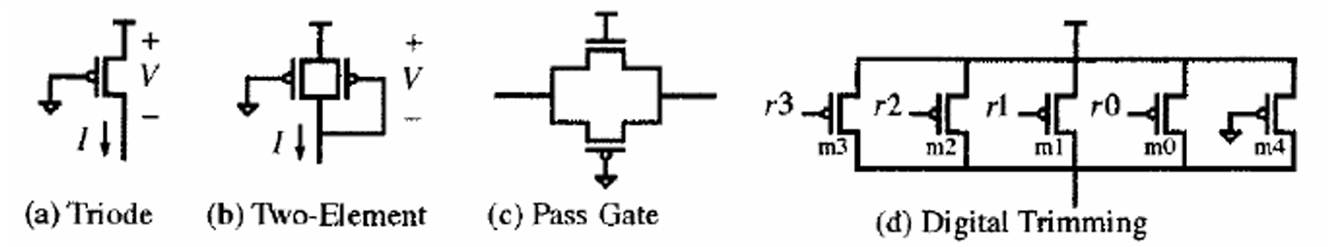
\includegraphics[width=0.9\linewidth]{1)active_termination.png}
    \caption{Active termination}
    \label{fig:active_term}
\end{figure}

% --- Second Image: Combination ---
\begin{figure}[htbp]
    \centering
    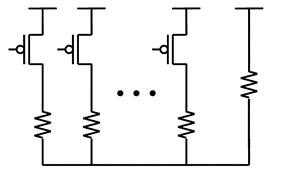
\includegraphics[width=0.4\linewidth]{2)combined_termination.png}
    \caption{Combination of Active and Passive}
    \label{fig:combined_term}
\end{figure}

\subsection{Equalization} \label{subsec:equalization}
\begin{itemize}
\item Equalization goal is to flatten the frequency response out to the Nyquist Frequency and remove time-domain ISI. TXs use pre-emphasis to shape their output spectrum (e.g., boosting high-frequency or de-emphasizing low-frequency content) , We usually use \textbf{de-emphasis} to not to increase Swing because we are limited by supply , EMI which will cause cross-talk , but at the cost of attenuated transmit signal

\item The number of taps and maximum tap weights determine allowable de-emphasis value and the quality of equalization both are usually specified by standards as more equalization , attenuates signal at small
frequency , so we limit this equalization because I have minimum eye opening

\item One approach to set the TX FIR coefficients is a \textbf{Minimum Mean-Square Error (MMSE) Algorithm}
\end{itemize}

\begin{figure}[htbp]
    \centering
    % 1. The Photo First
    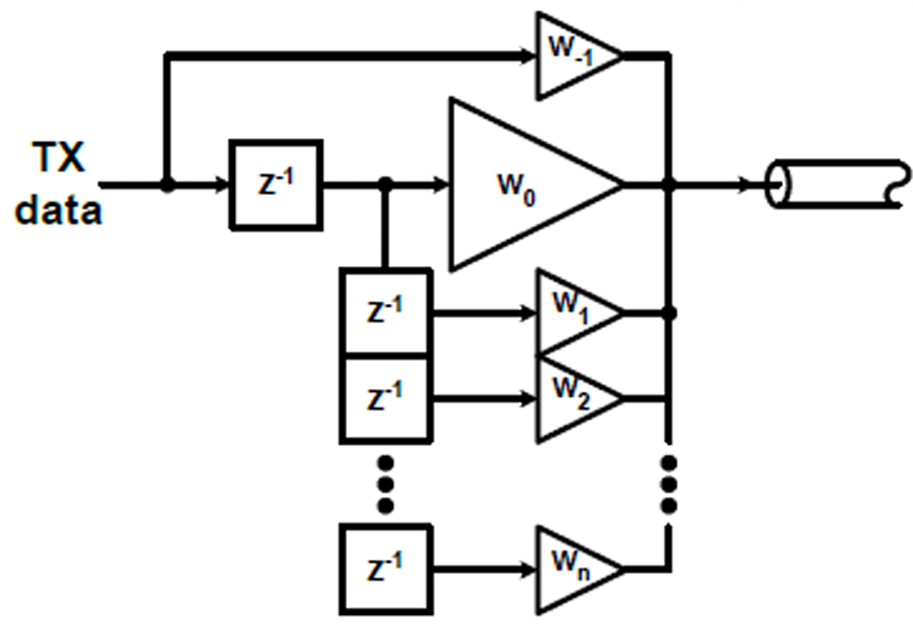
\includegraphics[width=0.5\textwidth]{3)Tx_FFE_Implementation.png}
    
    \vspace{10pt} 
    
    % 2. Mathematical representation exactly as requested
    \begin{center}
        \textbf{Low Frequency Response (Sum Taps)} \\
        $[\dots \enspace 1 \enspace 1 \enspace 1 \enspace \dots] * [-0.131 \enspace 0.595 \enspace -0.274] = [\dots \enspace 0.190 \enspace 0.190 \enspace 0.190 \enspace \dots]$ \\[10pt]
        \textbf{Nyquist Frequency Response (Sum Taps w/ Alternating Polarity)} \\
        $[\dots \enspace -1 \enspace 1 \enspace -1 \enspace \dots] * [-0.131 \enspace 0.595 \enspace -0.274] = [\dots \enspace 1 \enspace -1 \enspace 1 \enspace \dots]$
    \end{center}
    
    \vspace{5pt}
    
    % 3. The Caption at the very end
    \caption{Tx FFE Example}
    \label{fig:tx_ffe_example}
\end{figure}

\begin{figure}[htbp]
    \centering
    % --- Subfigure (a) ---
    \begin{subfigure}{0.32\textwidth}
        \centering
        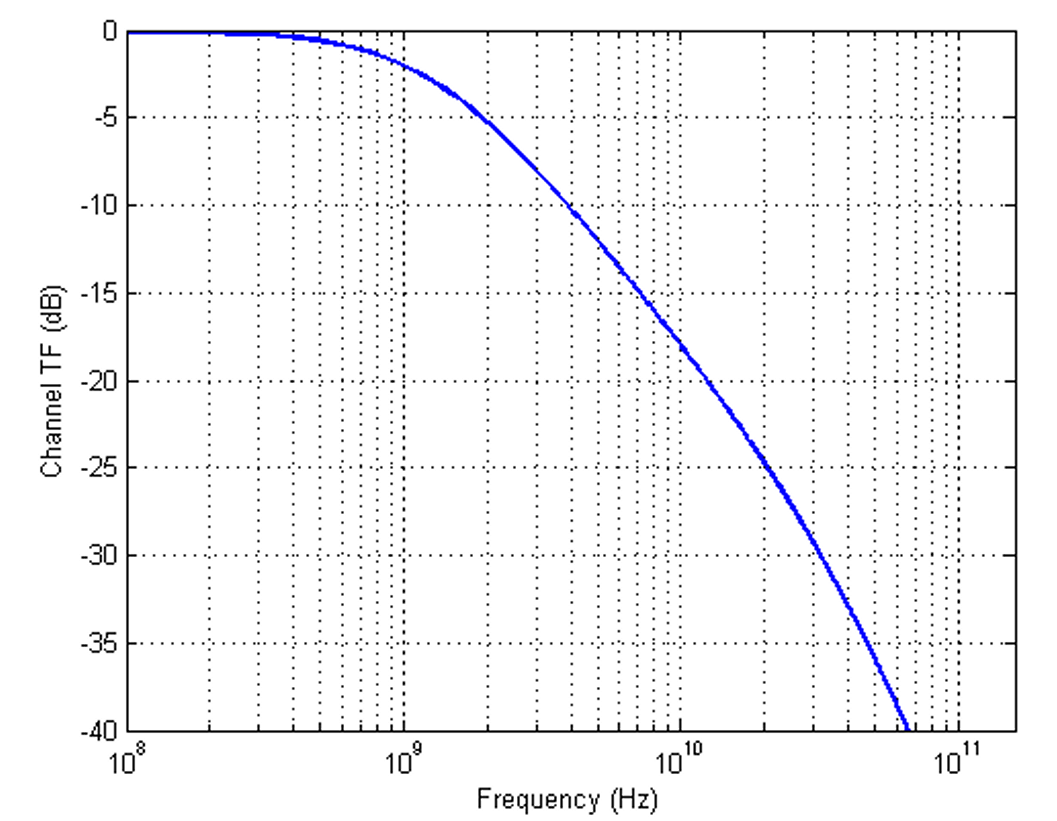
\includegraphics[width=\textwidth]{4.1)Channel_frequency_response.png}
        \caption{}
        \label{fig:channel_response}
    \end{subfigure}
    \hfill
    % --- Subfigure (b) ---
    \begin{subfigure}{0.32\textwidth}
        \centering
        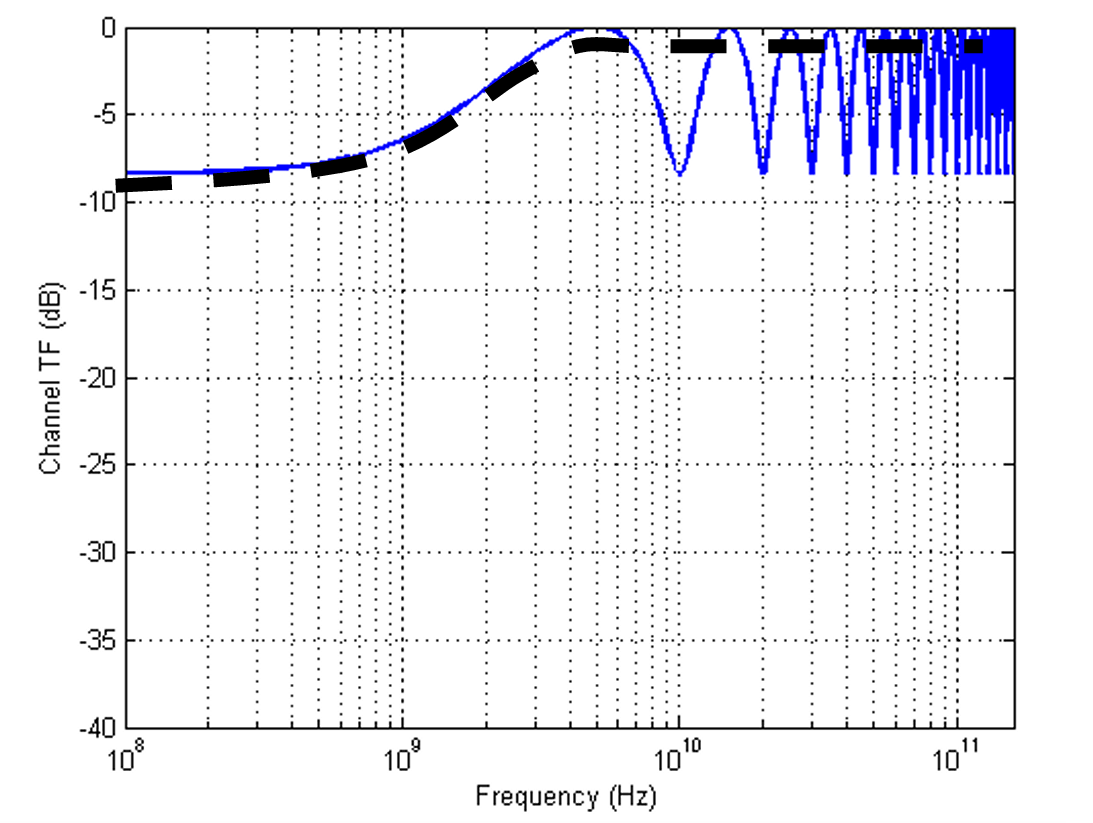
\includegraphics[width=\textwidth]{4.2)FIR_frequency_response.png}
        \caption{}
        \label{fig:fir_response}
    \end{subfigure}
    \hfill
    % --- Subfigure (c) ---
    \begin{subfigure}{0.32\textwidth}
        \centering
        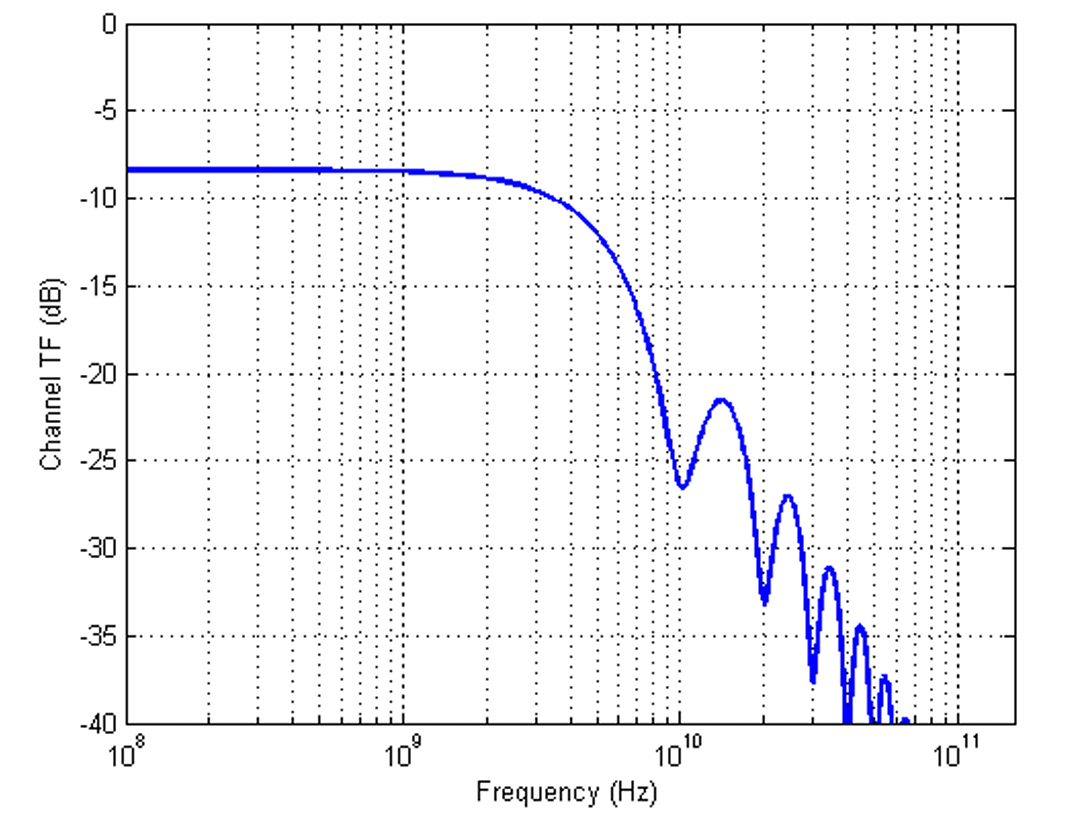
\includegraphics[width=\textwidth]{4.3)Combined_channel_and_Tx.png}
        \caption{}
        \label{fig:combined_response}
    \end{subfigure}

    \vspace{0.3cm}
    \caption{ (a) Channel frequency response ; (b) FIR frequency response ; (c) Combined channel and Tx}
    \label{fig:equalization_plots}
\end{figure}

\begin{figure}[H]
    \centering
    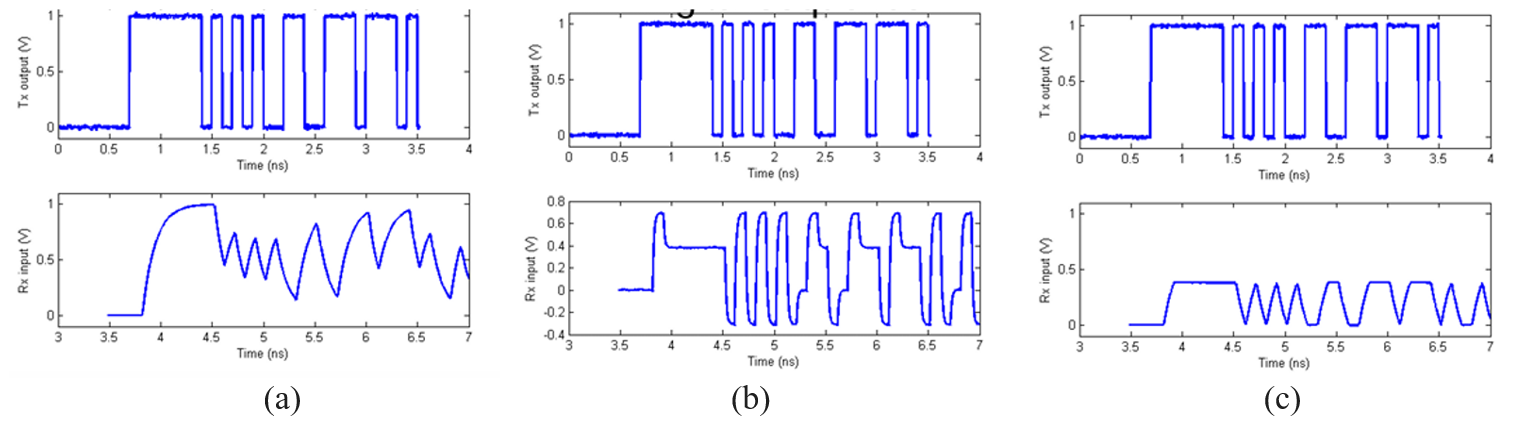
\includegraphics[width=1\textwidth ]{5)sent_data.png}
    \caption{(a) Tx and Rx signals with lossy channel without Tx EQ; (b) Tx Pre-distorted output to compensate for channel ISI; (c) Rx received signal with Tx EQ}
    \label{fig:sent_data}
\end{figure}

\begin{itemize}
\item If no Tx pre-emphasis is used the single bit transitions are heavily attenuated compared to CIDs
\item When Tx pre-emphasis is used the transition bits are emphasized, non transition but are not emphasized
\item The channel attenuates the transition bits more than the non transition bits due to their higher frequency content
\item At the receiver input both transition and non transition bits have the same amplitude, i.e. ISI is eliminated
\end{itemize}

\begin{figure}[H]
    \centering
    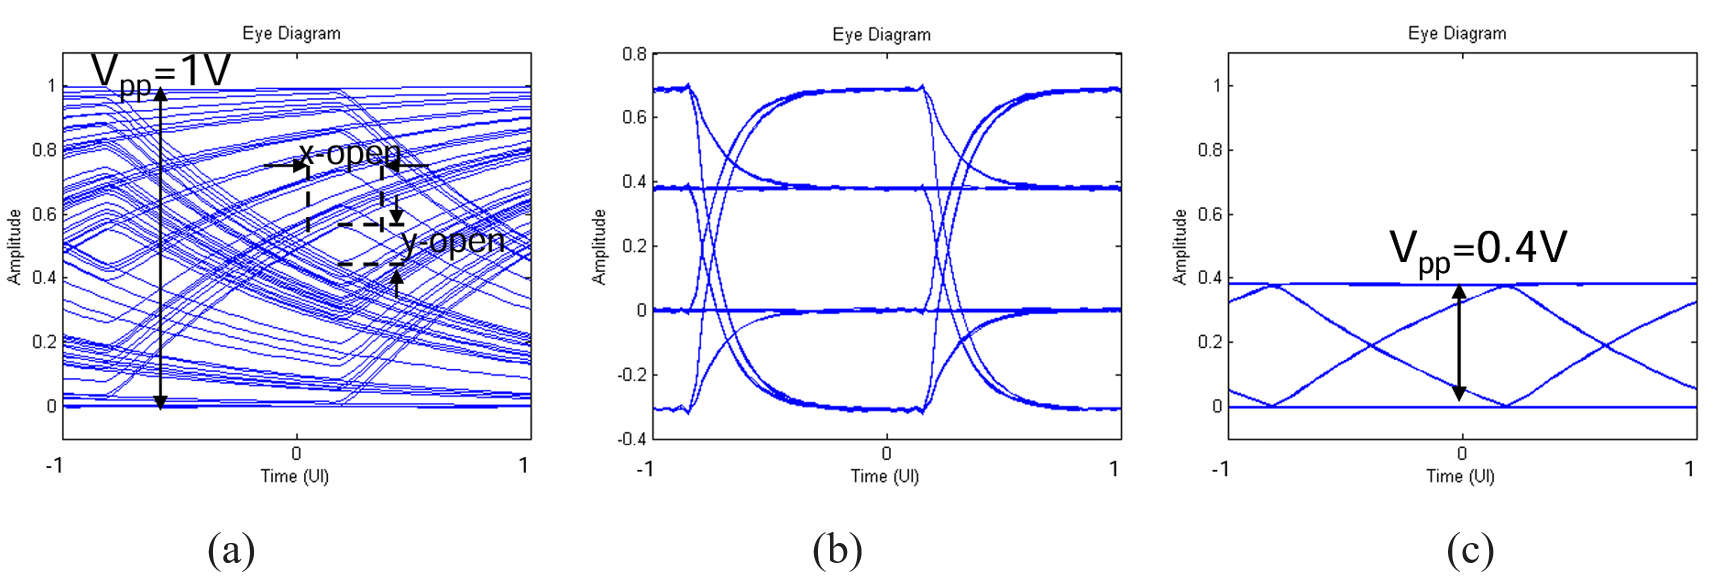
\includegraphics[width=1\textwidth ]{6)EYE.png}
    \caption{(a) RX eye diagram with lossy channel without Tx EQ; (b) Tx output eye diagram with pre-emphasis (pre-distorted eye); (c) Rx received eye diagram with Tx pre-emphasis}
    \label{fig:EYE}
\end{figure}

\begin{itemize}
\item Receiver eye was nearly closed without using Tx pre-emphasis resulting in high BER
\item After applying the right amount of pre-emphasis, ISI can be eliminated from the received eye
\item However, pre-emphasis also reduces the outer eye opening, i.e. the non 
transition bits are de-emphasized, thus a maximum limit is usually set by 
standards on how much pre-emphasis can be used

\end{itemize}

\section{Analog-based and DAC-based Drivers} \label{sec:Analog/DAC-based}

The implementation of Feed-Forward Equalization (FFE) generally falls into two categories based on how the tap summation and signal modulation are performed.

\subsection{Analog-based transmitters} \label{subsec:Analog-based}
In analog-based transmitters, the equalization is performed by summing currents or voltages of the taps directly at the output node.

\begin{itemize}
    \item \textbf{Implementation Idea:} Tap weights are implemented by adjusting the number of active slices for each cursor (Pre, Main, and Post).
    \item \textbf{FFE Taps and Clocking:} To achieve UI-spaced FFE taps, custom digital delay elements such as latches are required. For tap programmability, high-speed MUXs clocked with multiple phases (half- or quarter-rate) are necessary. This significantly increases the complexity of the clocking tree and the capacitive load, often forcing equalization and tap selection to be handled at higher speeds.
    \item \textbf{Modulation Challenges:} Supporting higher modulation techniques, such as PAM-4, requires multiple serializers (e.g., separate paths for MSB and LSB) for a single cursor. This increases the capacitive loading on the transmitter output, which degrades the output bandwidth and significantly increases power consumption and complexity as the number of taps grows.
\end{itemize}


 \begin{figure}[htbp]
     \centering
     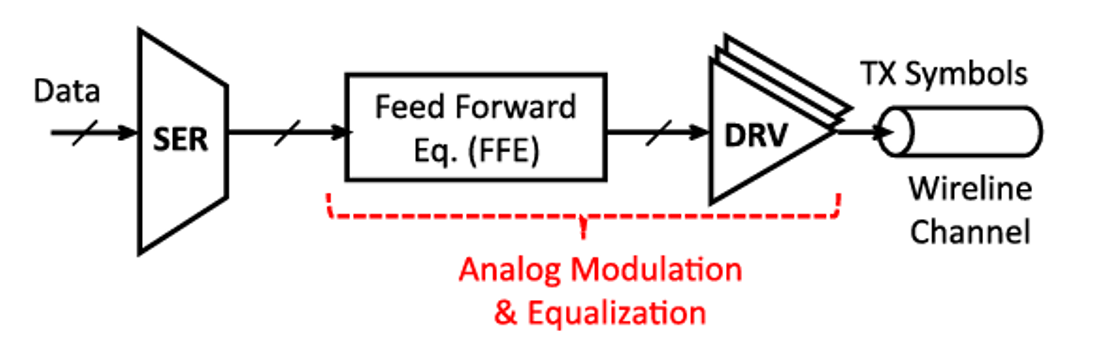
\includegraphics[width=0.8\textwidth]{7)Analog-based}
     \caption{Analog-based Transmitter Architecture.}
 \end{figure}

\subsection{DAC-based transmitters} \label{subsec:DAC-based}
DAC-based transmitters move the equalization and tap weight calculation into the digital domain, using a Digital to Analog Converter (DAC) as the final output stage.
DAC-based architectures the dominant choice for TXs with five or more FFE taps

\begin{itemize}
    \item \textbf{Implementation Idea:} Equalization is performed digitally within a DSP. The DSP outputs a digital code representing the required analog voltage for each bit sent into the channel.
    \item \textbf{FFE Taps and Clocking:} Both the generation of taps and their programmability are handled in the digital domain. This eliminates the need for high-speed analog delay elements or high-speed MUXs for tap selection. Consequently, the pre-driver circuitry is much simpler, and the load on the clocking distribution is reduced , helping equalization and tap selection to be handled at lower speeds .
    \item \textbf{Modulation Flexibility:} The driver functions as a DAC that represents the weight of the bit code. This structure remains the same regardless of the modulation technique used. This architecture offers superior flexibility for supporting advanced modulation schemes like PAM-4 or PAM-8 without the massive complexity scaling seen in analog designs.
\end{itemize}


\begin{figure}[htbp]
     \centering
     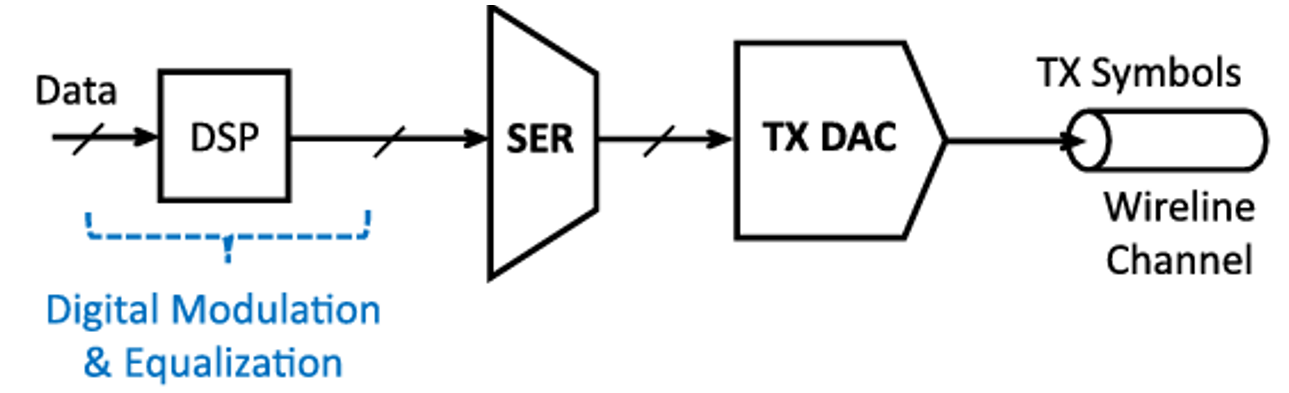
\includegraphics[width=0.8\textwidth]{8)DAC_Based}
     \caption{DAC-based Transmitter Architecture.}
 \end{figure}

 \subsubsection{Digital TX FFE} \label{ssubsec:DSP}

Digital TX FFEs are often implemented using Look-Up Tables (LUTs). A fully LUT-based implementation stores an $N$-tap filter span computation in an LUT, which requires an $N \cdot \log_2(M)$-bit address (for $M$-PAM modulation) and an output word width equal to the DAC resolution.

\begin{itemize}
    \item  For example, as shown in Fig.~\ref{fig:dac_ffe_lut_full}, a 2-PAM 4-tap FFE with 6-bit DAC resolution requires 16 rows and 6 columns, totaling 96 registers or memory cells. However, this architecture does not scale well for 4-PAM systems; a 7-tap FFE with 7-bit resolution would require $2^{14} \times 7 = 114,688$ registers.
    
    \item  Instead, a more efficient 4-PAM architecture, illustrated in Fig.~\ref{fig:dac_ffe_lut_per_tap}, uses per-tap LUTs to eliminate multipliers and employs digital adders to combine the tap values. This approach allows for simple 4-row LUTs per tap.
    
    \item Given the dramatic reduction in row count, the internal DSP resolution can be increased to 8 bits. This reduces quantization noise in the subsequent adders before the signal is finally quantized to the 7-bit DAC resolution.
    
    \item Using this per-tap approach, a 4-PAM 7-tap FFE can be implemented with only 224 registers ($7 \text{ taps} \times 4 \text{ rows} \times 8 \text{ bits}$), making it much more hardware-efficient.
\end{itemize}

\begin{figure}[htbp]
    \centering
    % --- Subfigure A ---
    \begin{subfigure}{0.35\textwidth} % Increased slightly for better visibility
        \centering
        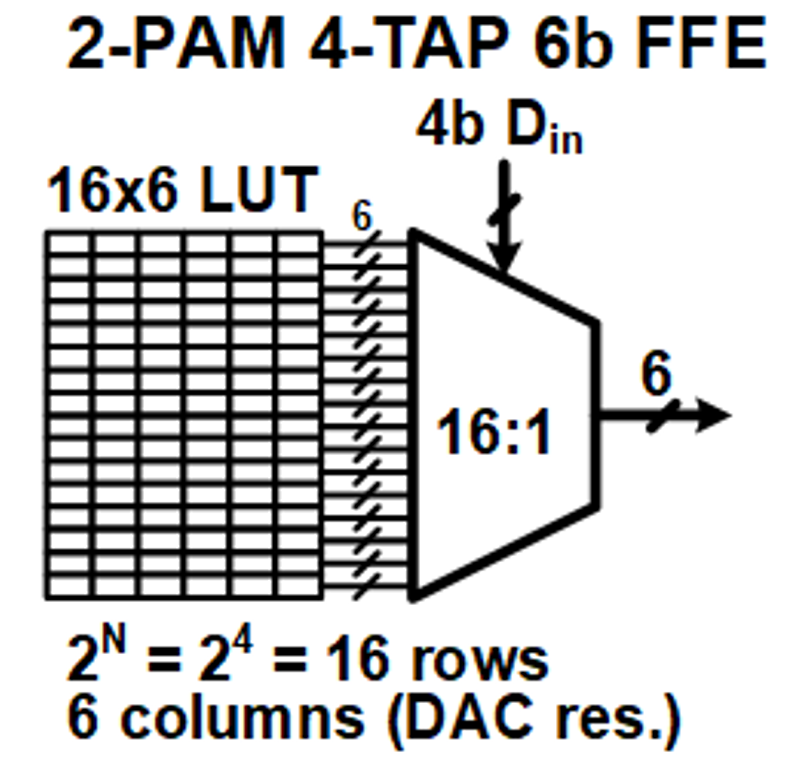
\includegraphics[width=\textwidth]{9)DAC_FFE_1.png}
        \caption{}
        \label{fig:dac_ffe_lut_full}
    \end{subfigure}
    \hfill % This pushes (a) to the left and (b) to the right
    % --- Subfigure B ---
    \begin{subfigure}{0.6\textwidth} % Adjusted to fill the remaining space
        \centering
        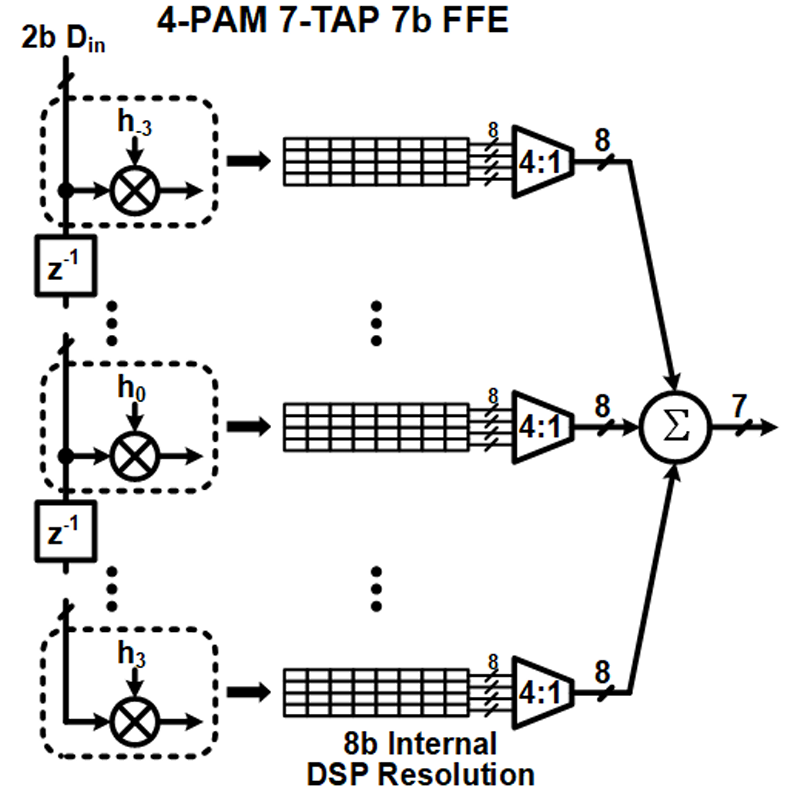
\includegraphics[width=\textwidth]{9)DAC_FFE_2.png}
        \caption{}
        \label{fig:dac_ffe_lut_per_tap}
    \end{subfigure}
    
    \vspace{0.3cm}
    \caption{Digital TX FFE implementations. (a) Fully LUT-based 2-PAM 4-tap FFE with 6b output resolution; (b) 4-PAM 7-tap FFE with tap-based LUTs and 7b output resolution.}
    \label{fig:dac_ffe_comparison}
\end{figure}
The reduction in register count is driven by the mathematical difference between \textbf{exponential growth} and \textbf{linear growth} as the number of taps ($N$) increases.

In the standard approach, a 7-tap 4-PAM system must account for every possible input combination ($4^7 = 16,384$ combinations) and gives the output directly. By treating each tap independently (multiplying each tap with its tap weight), the per-tap approach only needs to store 4 possible values for each of the 7 taps.
\begin{table}[htbp]
    \centering
    \caption{Comparison of the 2 Implementation Architectures}
    \label{tab:lut_comparison}
    \begin{tabular}{@{}lll@{}}
        \toprule
        \textbf{Feature} & \textbf{Fully LUT-Based Approach} & \textbf{Per-Tap LUT Approach} \\ \midrule
        Logic Basis & $2^{N \cdot \log_2(M)}$ rows & $M$ rows per tap \\
        Scaling for 4-PAM 7-Tap & Requires $2^{14}$ addresses & Requires $4$ rows $\times 7$ taps \\
        Total Registers & 114,688 registers & 224 registers \\ \bottomrule
    \end{tabular}
\end{table}

\section{Driver Topologies} \label{sec:Driver_topologies}
\subsection{Voltage Mode} \label{subsec:Voltage_mode}
\subsubsection{NRZ SST} \label{ssubsec:NRZ_SST}

\begin{figure}[H]
    \centering
    % --- Subfigure (a) ---
    \begin{subfigure}{0.4\linewidth}
        \centering
        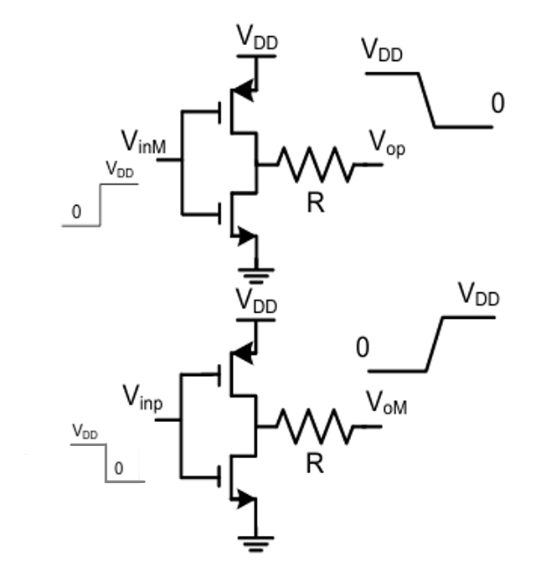
\includegraphics[width=\textwidth]{10)SST}
        \caption{}
        \label{fig:SST}
    \end{subfigure}
    \hfill
    % --- Subfigure (b) ---
    \begin{subfigure}{0.21\linewidth}
        \centering
        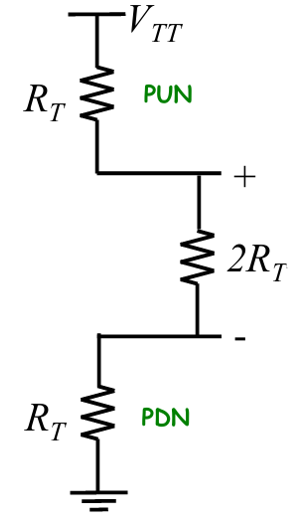
\includegraphics[width=\textwidth]{10.1)Equivalent_Circuit}
        \caption{}
        \label{fig:Equivalent Circuit_NRZ}
    \end{subfigure}
    \hfill
    \vspace{0.3cm}
    \caption{ (a) SST ; (b) Equivalent Circuit}
    \label{fig:NRZ SST}
\end{figure}

\begin{itemize}
    \item SST driver consists of inverters driving series termination resistors.
    \item Actual source impedance is a series combination of $R_{TERM}$ and $Z_{NMOS}$ or $Z_{PMOS}$.
    \item The series resistors provide ESD protection for transistors’ drain junctions.
    \item Transistor impedance varies with region of operation and PVT corners.
    \item Differential peak-to-peak output swing is equal to $V_{DD}$.
\end{itemize}


\subsubsection{PAM-4 SST} \label{ssubsec:PAM-4_SST}

\begin{figure}[H]
    \centering
    % --- Top Row ---
    \begin{subfigure}[t]{0.48\linewidth} % Adjusted to fit side-by-side
        \centering
        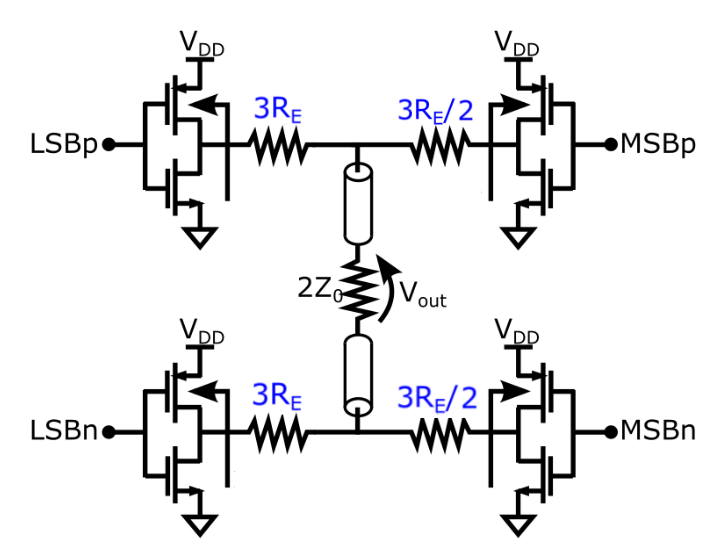
\includegraphics[width=\textwidth]{11)PAM4_SST}
        \caption{2-bit (PAM-4) SST Architecture}
        \label{fig:PAM4_SST_Circuit}
    \end{subfigure}
    \hfill % Pushes subfigures to the edges
    \begin{subfigure}[t]{0.48\linewidth} % Adjusted to fit side-by-side
        \centering
        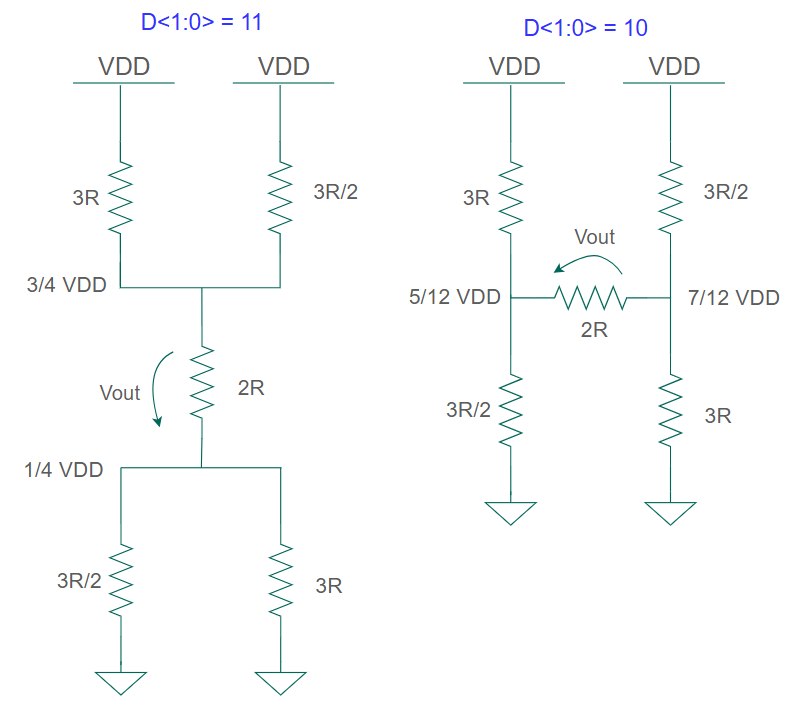
\includegraphics[width=\textwidth]{11.2)Equivalent_Circuit_PAM4}
        \caption{Equivalent Circuit}
        \label{fig:Equivalent_Circuit_PAM4}
    \end{subfigure}

    \vspace{0.5cm} % Adds vertical space before the next row

    % --- Bottom Row (A blank line above this forces it down) ---
    \begin{subfigure}[t]{0.6\linewidth} % Larger width for the centered EYE
        \centering
        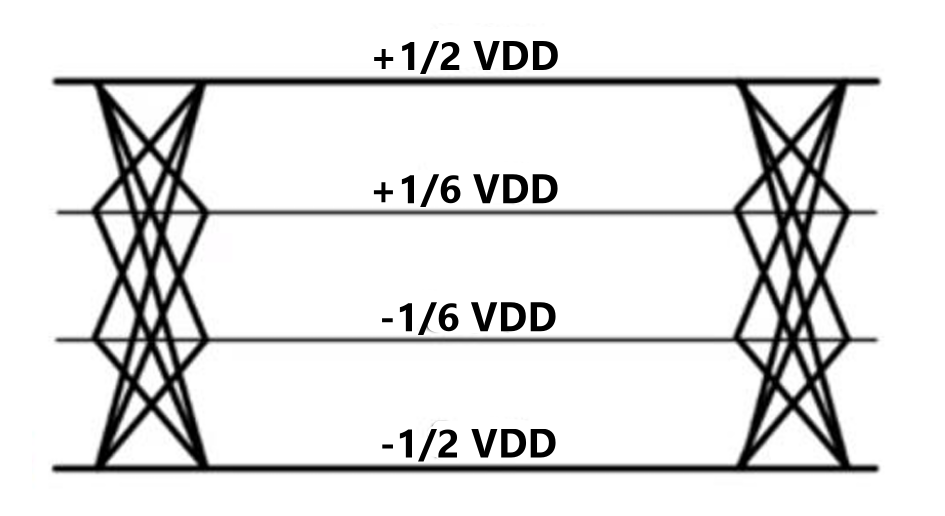
\includegraphics[width=\textwidth]{11.3)EYE}
        \caption{EYE Diagram}
        \label{fig:sttpam4eye}
    \end{subfigure}
    
    \caption{}
    \label{fig:PAM-4_SST_Main}
\end{figure}


\begin{itemize}
\item It can be Considered as a 2 bit DAC
\item voltage divider is made for each input
\end{itemize}


\subsection{Current Mode} \label{subsec:Current_mode}
\subsubsection{NRZ CML} \label{ssubsec:NRZ_CML}
 \begin{figure}[H]
     \centering
     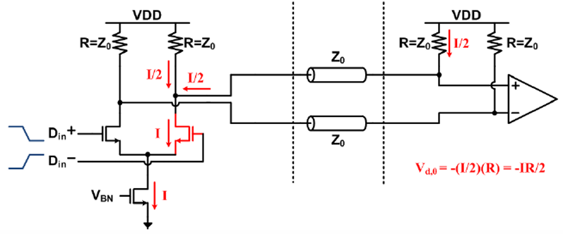
\includegraphics[width=0.8\textwidth]{12)CML}
     \caption{Conventional CML.}
 \end{figure}
 \begin{itemize}
    \item Differential pair steers the current into a differential I/O link.
    \item Differential pp RX swing is \textbf{$\pm IR/2$.}
    \item Note that \textbf{Swing = IR} and \textbf{Vo,CM = VDD-IR/2}, so by ignoring supply variations, we can have precise Swing and CM by using I outputted from Bandgap which track $1/R$ and use poly resistor so If R shifted I will shift opposite to it So swing and CM become constant.
    \item For high swing (Large current) we will need large i/p pair to have lower $V_{GS}$ and preserve current source in Sat. For ex: $0.8V_{pp}$ swing needs $I_B=16mA$ (w/o taking current mirrors into considerations).
    \item So a pre-driver is necessary to drive the large capacitance of the output stage (chain of inverters).
    \item Tradeoffs between Power, speed, swing, BER.
\end{itemize}


\clearpage
\subsubsection{PAM-4 CML} \label{ssubsec:PAM-4_CML}
\begin{figure}[H]
    \centering
    % --- Top Row ---
    \begin{subfigure}[t]{0.48\linewidth} % Adjusted to fit side-by-side
        \centering
        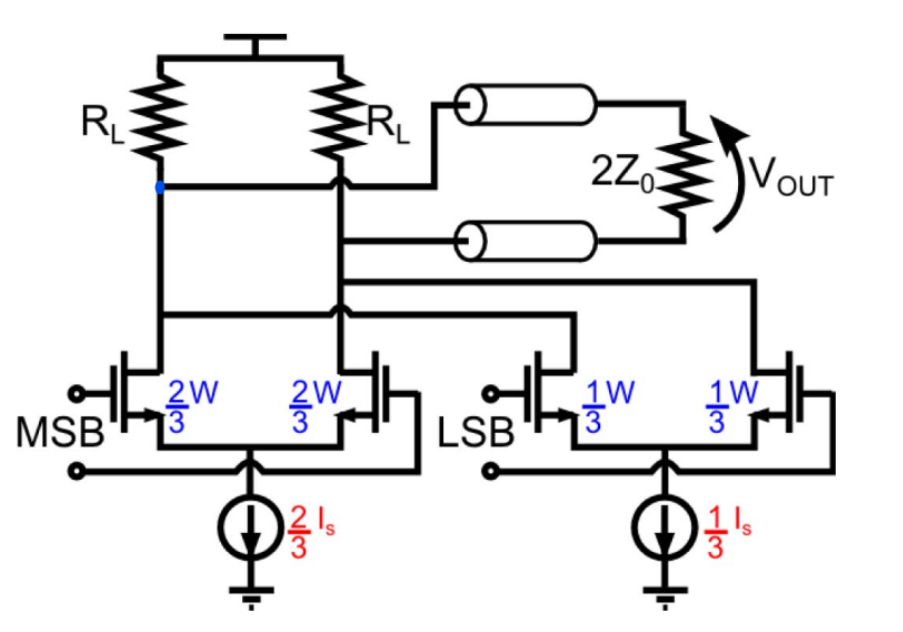
\includegraphics[width=\textwidth]{13)PAM4CML}
        \caption{2-bit (PAM-4) CML Architecture}
        \label{fig:PAM4_SST_Circuit}
    \end{subfigure}
    \hfill % Pushes subfigures to the edges
    \begin{subfigure}[t]{0.51\linewidth} % Adjusted to fit side-by-side
        \centering
        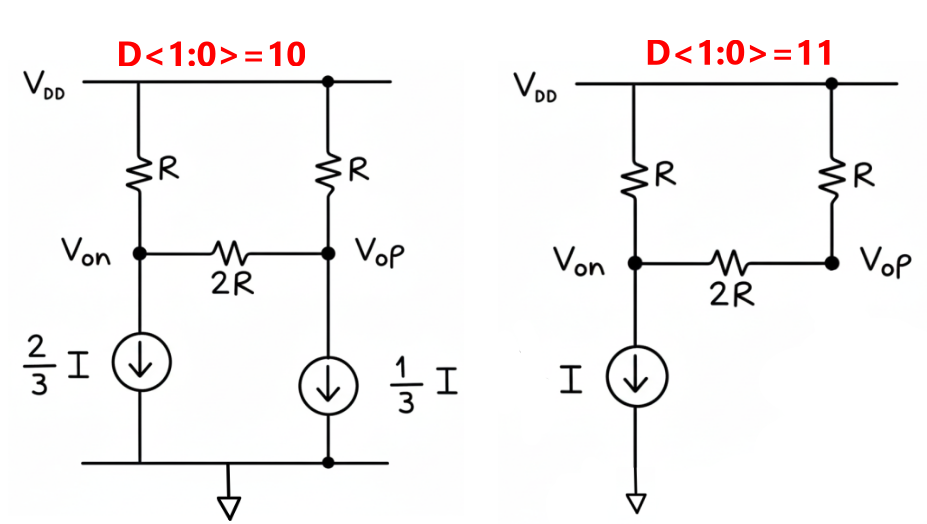
\includegraphics[width=\textwidth]{13.1)Equiv_cir}
        \caption{Equivalent Circuit}
        \label{fig:Equivalent_Circuit_PAM4}
    \end{subfigure}

    \vspace{0.5cm} % Adds vertical space before the next row

    % --- Bottom Row (A blank line above this forces it down) ---
    \begin{subfigure}[t]{0.5\linewidth} % Larger width for the centered EYE
        \centering
        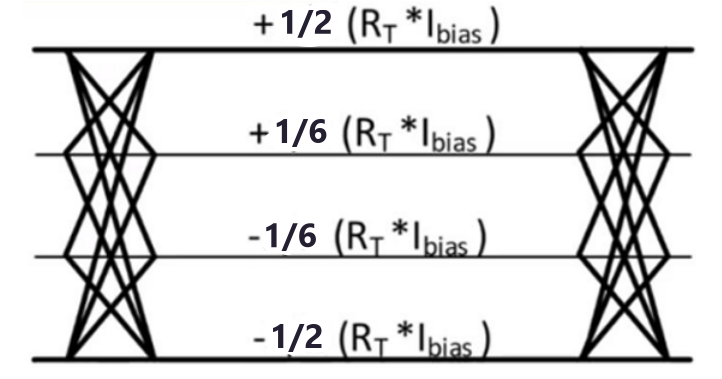
\includegraphics[width=\textwidth]{13.2)EYE}
        \caption{EYE Diagram}
        \label{fig:sttpam4eye}
    \end{subfigure}
    
    \caption{}
    \label{fig:PAM-4_SST_Main}
\end{figure}
\noindent \textbf{For D<1:0>=10:} 

\begin{enumerate}
    \item \textbf{KCL at node $V_{on}$}:
    \begin{equation}
        \frac{V_{DD} - V_{on}}{R} + I_{2R} = \frac{2}{3}I \label{eq:kclnodevon10}
    \end{equation}
    
    \item \textbf{KCL at node $V_{op}$}:
    \begin{equation}
        \frac{V_{DD} - V_{op}}{R} - I_{2R} = \frac{1}{3}I \label{eq:kclnodevop10}
    \end{equation}
\end{enumerate}

Subtracting equation \eqref{eq:kclnodevop10} from equation \eqref{eq:kclnodevon10} yields:
\begin{equation}
    \frac{V_{op} - V_{on}}{R} + 2I_{2R} = \frac{1}{3}I
    \label{eq:substpam4cml}
\end{equation}

By Ohm's Law, the differential voltage is defined as $V_{op} - V_{on} = I_{2R}(2R)$ . Substituting this into equation \eqref{eq:substpam4cml}:
\begin{equation}
    \frac{2R \cdot I_{2R}}{R} + 2I_{2R} = \frac{1}{3}I
\end{equation}

\begin{equation}
    4I_{2R} = \frac{1}{3}I \implies I_{2R} = \frac{1}{12}I
\end{equation}

This result confirms that the current passing through the bridging resistor is exactly $1/12$ of the total tail current $I$ 
\begin{align}
    V_{diff} &= +\frac{1}{12}I \times 2R \label{eq:vout_step} \\
    &= +\frac{1}{6}IR \label{eq:vout_final}
\end{align}
\noindent \textbf{For D<1:0>=11:} 
\begin{enumerate}
    \item \textbf{KCL at node $V_{on}$}:
    \begin{equation}
        \frac{V_{DD} - V_{on}}{R} + I_{2R} = I_s
        \label{eq:eq1pam4cml}
    \end{equation}
    
    \item \textbf{KCL at node $V_{op}$}:
    \begin{equation}
        \frac{V_{DD} - V_{op}}{R} - I_{2R} = 0
         \label{eq:eq2pam4cml}
    \end{equation}
\end{enumerate}

Subtracting equation \eqref{eq:eq2pam4cml} from equation \eqref{eq:eq1pam4cml} to isolate the differential terms:
\begin{equation}
    \frac{V_{op} - V_{on}}{R} + 2I_{2R} = I_s
\end{equation}

Applying Ohm's Law for the bridging resistor, where $V_{op} - V_{on} = I_{2R}(2R)$ 
\begin{equation}
    \frac{2R \cdot I_{2R}}{R} + 2I_{2R} = I_s
\end{equation}

\begin{equation}
    4I_{2R} = I_s \implies I_{2R} = \frac{1}{4}I_s
\end{equation}

The differential output voltage $V_{diff}$ is then calculated as:
\begin{equation}
    V_{diff} = I_{2R}(2R) = \left( \frac{1}{4}I_s \right)(2R) = \frac{1}{2}I_sR
\end{equation}

\subsubsection{H-bridge CML} \label{ssubsec:H_CML}

 \begin{figure}[H]
     \centering
     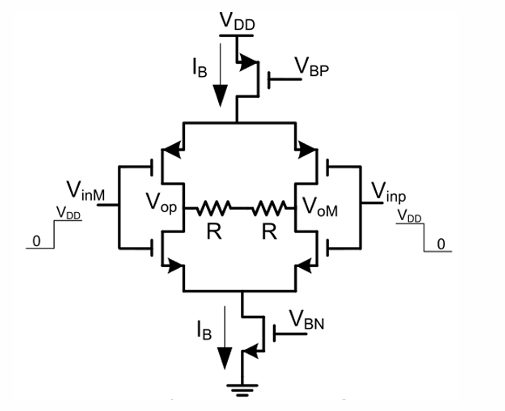
\includegraphics[width=0.5\textwidth]{14)H-bridge}
     \caption{H-Bridge}
 \end{figure}
 \begin{itemize}
    \item \textbf{Output Swing Calculation}:  $V_{oPP,diff} = 2I_B R$ .
    \item \textbf{Power and Area Trade-offs}: Swing is doubled for the same power consumption but requires a larger circuit area . For the same swing as CML, we need $1/2$ the size of the NMOS input pair, but the addition of PMOS transistors with sizes larger than $1/2$ the area of the CML NMOS increases parasitic capacitance .
    \item \textbf{Headroom and Common-Mode (CM) Challenges}: The presence of two series current sources occupies a large voltage headroom . Furthermore, the output CM is not inherently defined; this can be resolved using a CMFB (Common-Mode Feedback) loop or by implementing a hybrid topology .
    \item \textbf{Hybrid Topology}: In a hybrid configuration, the SST defines the output CM, and the CML adds its swing on top of it; however, this approach increases self-loading .
\end{itemize}

\subsubsection{Tailless} \label{ssubsec:Tailless}
 \begin{figure}[H]
     \centering
     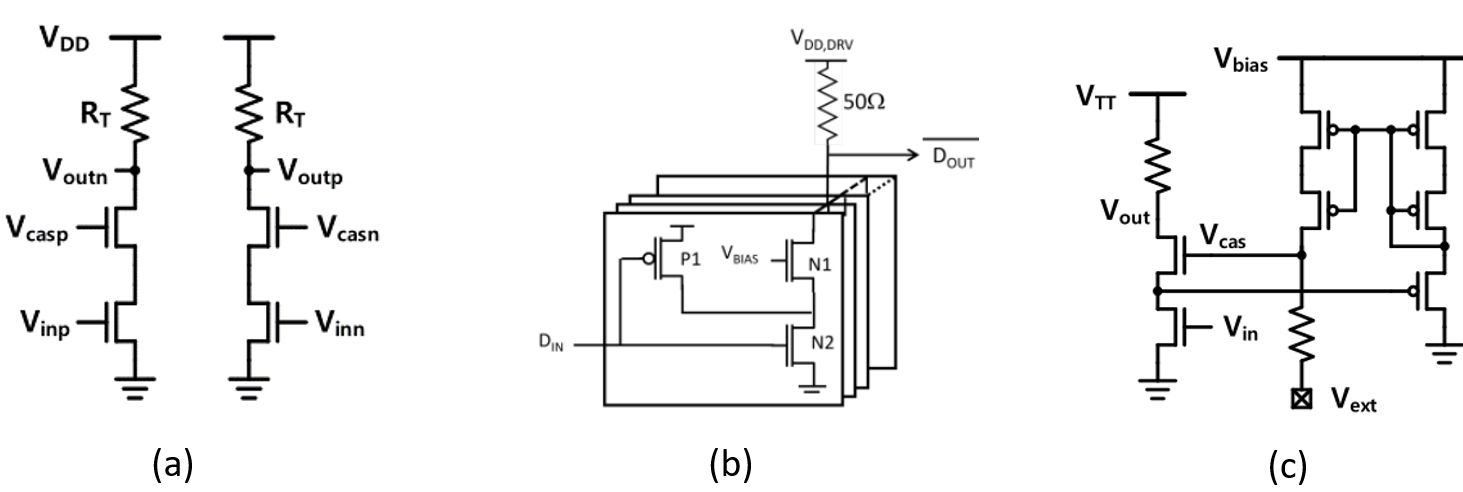
\includegraphics[width=1\textwidth]{16)Tailless}
     \caption{Tailless}
 \end{figure}
The tailless driver architecture offers significant advantages for high-speed data transmission by optimizing the transistor biasing and reducing parasitic effects.

\begin{itemize}
    \item \textbf{Device Operation}: The tailless driver consists of switching and cascode transistors that are flipped from the input and tail current source used in standard CML drivers. This configuration requires only the cascode (Casc) devices to remain in the saturation region for proper operation and they are whom defines current and though swing.
    
    \item \textbf{Parasitic Reduction}: By eliminating the tail current source, the $V_{GS}$ of the input pair can be increased. This allows the driver to deliver the same current (and thus the same output swing) using a smaller input pair, which significantly decreases parasitic capacitance. However, a high overdrive voltage ($V_{OV}$) must be managed to prevent transistors from entering the linear region.
    
    \item \textbf{Device Protection}: The $V_{DS}$ of the switches is determined by the $V_{GS}$ of the cascode transistors. Applying an appropriate $V_{casc}$ protects the input transistors from large output swings, enabling the use of thin-oxide devices which are essential for achieving the final high data rate.
    
    \item \textbf{Current Control}: In specific configurations, the P1 in fig(b) can disable current flow in the driver by pulling the source of N1 to the supply voltage when the digital input ($DIN$) is low.
    
    \item \textbf{Output Impedance ($R_{out}$)}: The cascode transistors are the primary devices forcing current, typically requiring a high channel length ($L$). However, since they connect directly to the output, $L$ is kept small to avoid increasing parasitics. To compensate and boost $R_{out}$, a "super $g_m$" configuration is  in fig(c), which is further amplified by the loop gain ($LG$).
\end{itemize}

\subsection{Hybrid Mode} \label{subsec:Hybrid_mode}

 \begin{figure}[H]
     \centering
     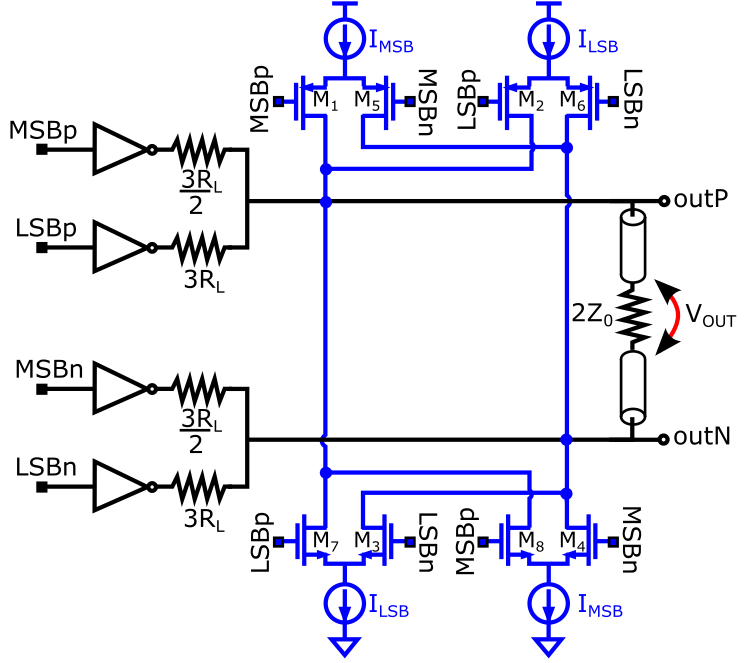
\includegraphics[width=0.6\textwidth]{17)Hybrid}
     \caption{Hybrid voltage and current mode}
 \end{figure}
Since V.mode max swing is VDD and CML high swings will give high non linearity , Hybrid topology is proposed to make the best compromise of them 
in addition to increasing the output swing above VDD

\begin{equation}
    V_{OUT,11} = V_{DD} + 2R_L I_s = V_{DD} + \Delta V
\end{equation}

\begin{equation}
    V_{OUT,10} = \frac{V_{DD}}{3} + \frac{2R_L I_s}{3} = \frac{V_{DD}}{3} + \frac{\Delta V}{3}
\end{equation}

 \begin{figure}[H]
     \centering
     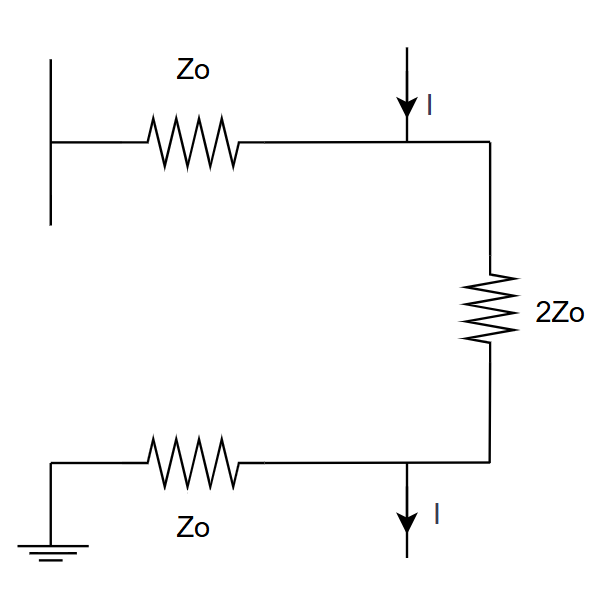
\includegraphics[width=0.3\textwidth]{ 17.1)Hybridnote}
     \caption{}
 \end{figure}
The CML is made as H-bridge to make all the current pass through the RX termination and prevent it from going to TX term 
\subsection{Comparison} \label{subsec:comp}
\subsubsection{Power} \label{ssubsec:Power}
\begin{figure}[H]
     \centering
     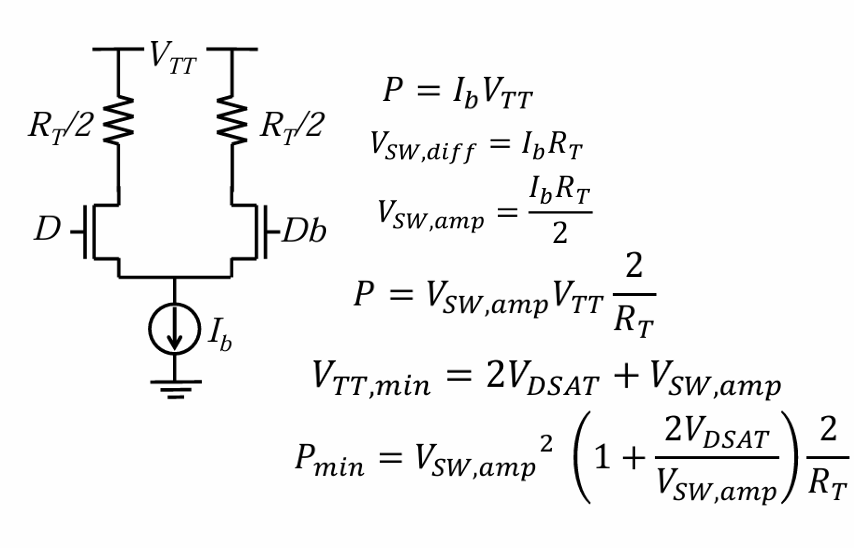
\includegraphics[width=0.7\textwidth]{18.1)powercml}
     \caption{}
 \end{figure}
 \begin{figure}[H]
     \centering
     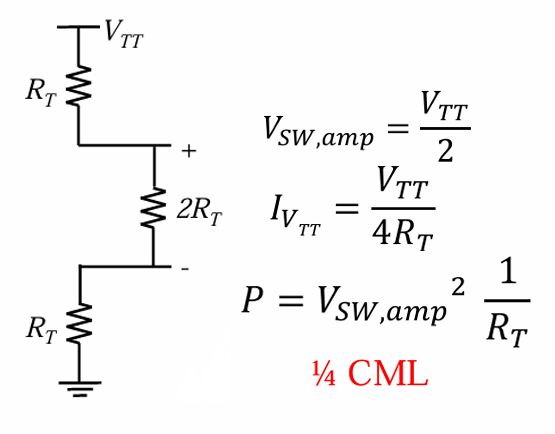
\includegraphics[width=0.7\textwidth]{18.2)powersst}
     \caption{}
 \end{figure}
 \clearpage
 
 \subsubsection{Swing} \label{ssubsec:Swing}
\begin{figure}[H]
    \centering
    % --- Subfigure A ---
    \begin{subfigure}{0.65\textwidth} % Increased slightly for better visibility
        \centering
        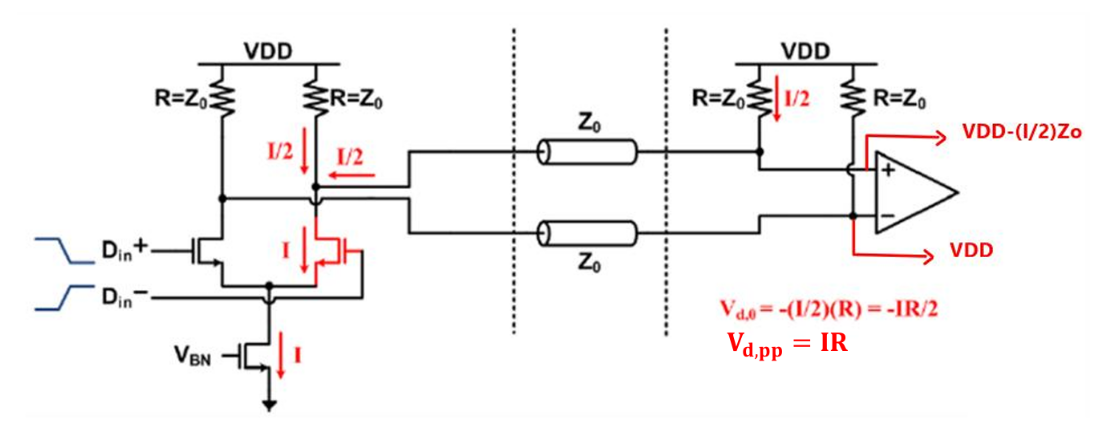
\includegraphics[width=\textwidth]{15)comp1}
        \caption{}
        \label{fig:dac_ffe_lut_full}
    \end{subfigure}
    \hfill % This pushes (a) to the left and (b) to the right
    % --- Subfigure B ---
    \begin{subfigure}{0.6\textwidth} % Adjusted to fill the remaining space
        \centering
        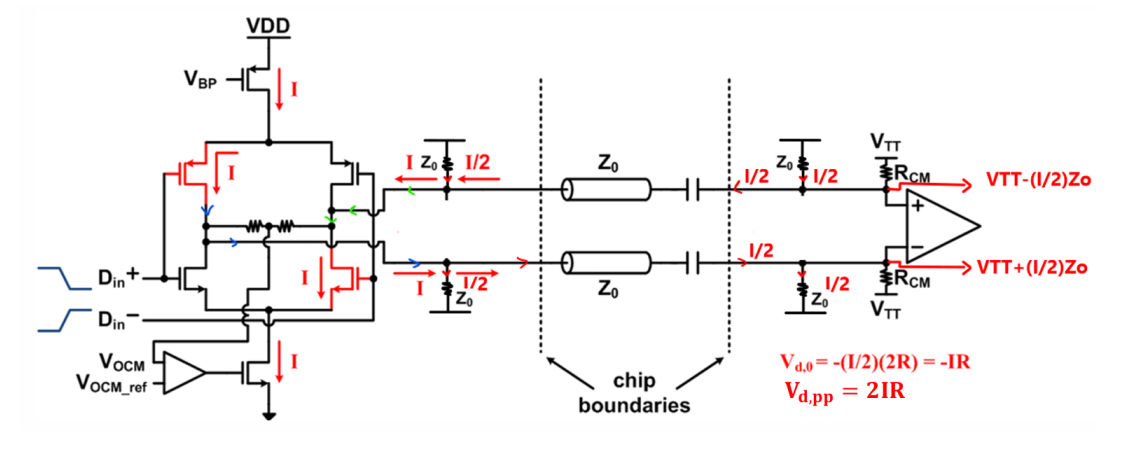
\includegraphics[width=\textwidth]{15)comp2}
        \caption{}
        \label{fig:dac_ffe_lut_per_tap}
    \end{subfigure}
    
    \vspace{0.3cm}
    \caption{CML Swings for SE termination. (a) CML; (b) H-bridge.}
    \label{fig:dac_ffe_comparison}
\end{figure}
\noindent \textbf{For CML : }
Total current is passing in one branch
\noindent \textbf{For H-Bridge :}
Total Current is passing in each of the 2 branches
• Current is divided equally between TX termination and RX termination
• ½  of the current reached to each SE  termination of the receiver
\begin{figure}[H]
    \centering
    % --- Subfigure A ---
    \begin{subfigure}{0.65\textwidth} % Increased slightly for better visibility
        \centering
        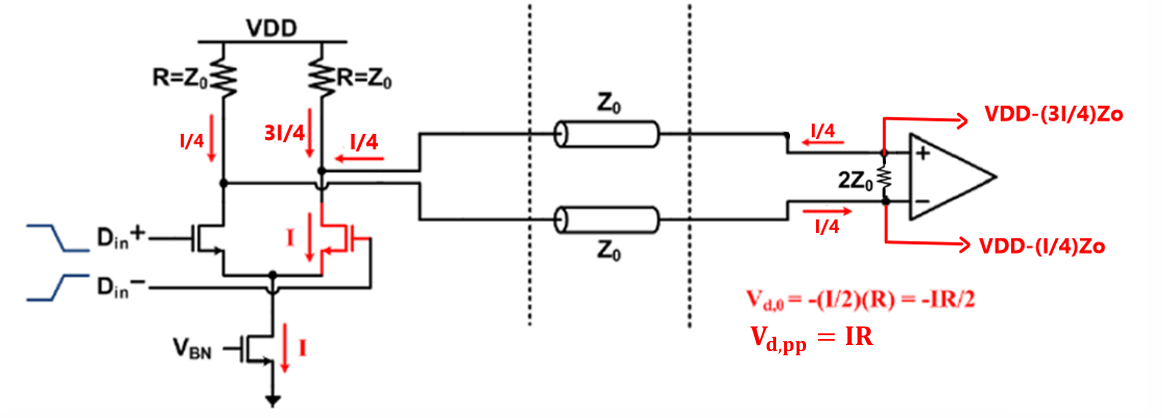
\includegraphics[width=\textwidth]{15)comp3}
        \caption{}
        \label{fig:dac_ffe_lut_full}
    \end{subfigure}
    \hfill % This pushes (a) to the left and (b) to the right
    % --- Subfigure B ---
    \begin{subfigure}{0.65\textwidth} % Adjusted to fill the remaining space
        \centering
        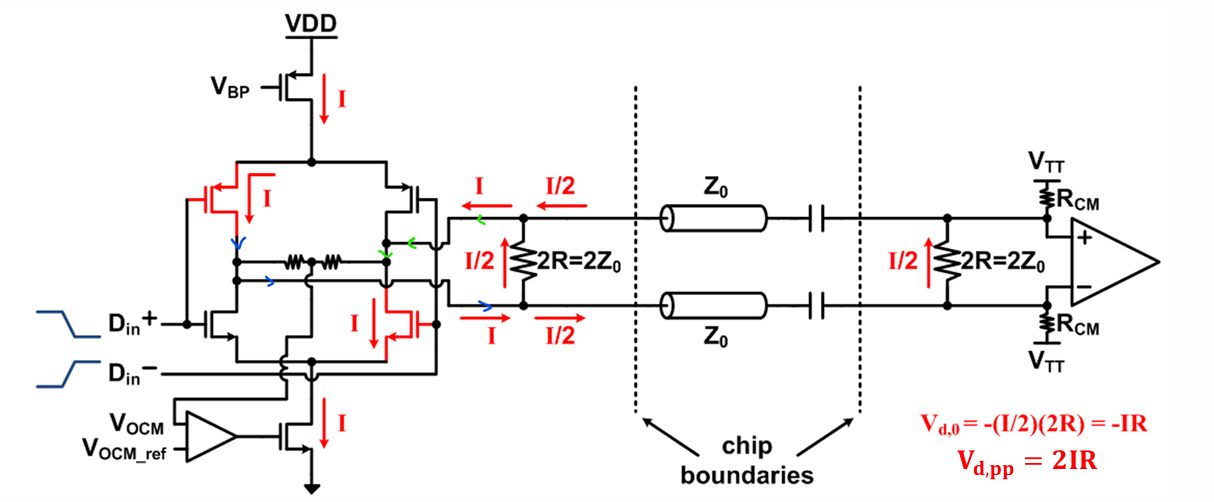
\includegraphics[width=\textwidth]{15)comp4}
        \caption{}
        \label{fig:dac_ffe_lut_per_tap}
    \end{subfigure}
    
    \vspace{0.3cm}
    \caption{CML Swings for Differential termination. (a) CML; (b) H-bridge.}
    \label{fig:dac_ffe_comparison}
\end{figure}

\noindent \textbf{For CML : }
\begin{itemize}
    \item at D=VDD , Db=0 :
    \begin{align}
        V_1 &= V_{DD} - \frac{3}{4} I_b R_T \\
        V_2 &= V_{DD} - \frac{1}{4} I_b R_T
    \end{align}
    \item ¼ of the current reached the differential Termination of the receiver
    \item The 2nd termination of TX became series with RX termination
\end{itemize}
\noindent \textbf{For H-Bridge :}
Total Current is passing in each of the 2 branches
• Current is divided equally between TX termination and RX termination
• ½  of the current reached the differential Termination of the receiver
 \begin{figure}[H]
     \centering
     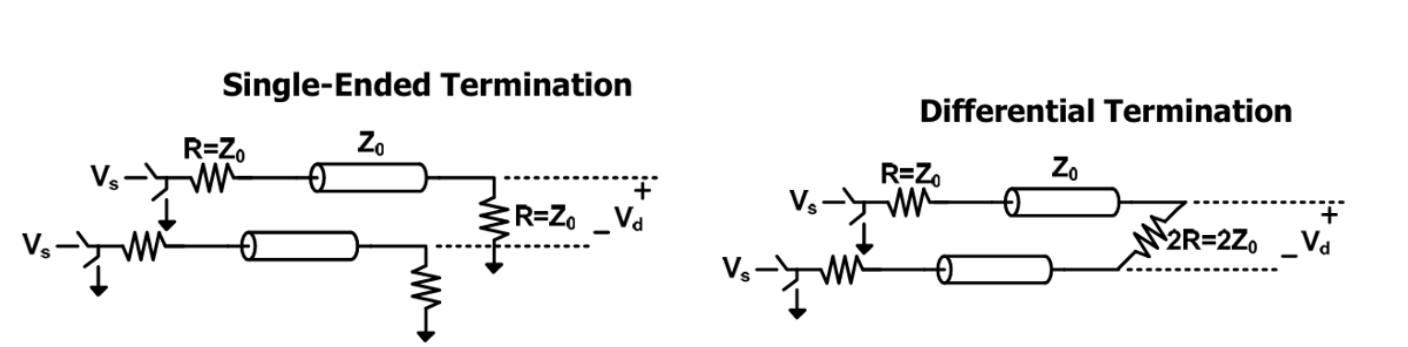
\includegraphics[width=1\linewidth]{10.2)Swings}
     \caption{ SST Swings a) SE Termination ; b) Differential Termination}
 \end{figure}
 
\noindent \textbf{For SE termination:}
\begin{align}
    V_{d,1} &= (Vs/2) & V_{d,0} &= -(Vs/2) \\
    V_{d,pp} &= Vs & I &= \frac{V_{d,pp}}{2R}              
\end{align}

\vspace{0.5cm}

\noindent \textbf{For Differential termination:}
\begin{align}
    V_{d,1} &= (Vs/2) & V_{d,0} &= -(Vs/2) \\
    V_{d,pp} &= Vs & I &= \frac{V_{d,pp}}{4R}     
\end{align}
\clearpage
 \subsubsection{Summary} \label{ssubsec:Summary}
\begin{table}[htbp]
    \centering
    \caption{Comparison Between Current Mode and Voltage Mode Driver Topologies}
    \label{tab:driver_comparison}
    \begin{tabularx}{\textwidth}{l X X}
        \toprule
        \textbf{Feature} & \textbf{Current Mode} & \textbf{Voltage Mode} \\
        \midrule
        \textbf{Swing} & Swing is set by current . & Swing is set by Supply. \\
        \addlinespace
        \textbf{Termination} & termination is set by $Z_0$ at high $R_{out}$. &  termination set by $Z_0$ and devices. \\
        \addlinespace
        \textbf{Power} & Static power; Less power efficient for same swing. & Dynamic power;  but for high speed , the very fast transitions can be averaged to be compared with static current,  more power efficient for same swing. \\
        \addlinespace
        \textbf{Speed} & faster due to constant current source activation  &  it is slower as it depends on charging and discharging caps \\        

        \addlinespace
        \textbf{SSO} & Static steered current prevents fast transitions. & Fast transitions can lead to supply bounce if parasitic inductors are present. \\
        \addlinespace
        \textbf{Programmability} & Swing is analog-programmed via current source without altering driver impedance. & Harder termination controllability ($R_{ON}$ depends on $\mu, V_{th}$, etc.). Analog Tuning through header/footer CSs degrades linearity. \\
        \addlinespace
        \textbf{Linearity} & Degraded linearity as current source operates in different regions during transitions. & Better linearity; series resistance overcomes $R_{ON}$ non-linearity. \\
        \addlinespace
        \textbf{Trade-offs} & Swing $\uparrow$, $V_{oCM} \downarrow$, headroom $\downarrow$, linearity $\downarrow$ (tail operates close to triode). Input size $\uparrow$, headroom for tail $\uparrow$, BW $\downarrow$. & Linearity vs. Speed trade-off. Increasing $Z_0/R_{ON}$ improves linearity but degrades bandwidth (BW). \\
        \bottomrule
    \end{tabularx}
\end{table}


\clearpage
% ==================================================
% CHAPTER 3: IMPLEMENTATION (OUTLINE)
% ==================================================
\chapter{Circuit Implementation and Optimization Strategy}
\label{ch:implementation}

\section{I/Q Divider}

The IQ Divider is the primary frequency-translation element in the transmitter clocking path, responsible for converting the high-frequency PLL output into multiple phases at a lower fundamental frequency.

\subsection{Architecture and Operation}
The most common implementation for generating precise quadrature phases at high frequencies is a \textbf{Divide-by-2 circuit} composed of two cascaded differential static latches (Master and Slave) configured in a negative feedback loop.

\begin{itemize}
    \item \textbf{Master-Slave Configuration:} The two latches are connected in series, with the output of the slave latch cross-coupled and fed back to the input of the master latch.
    
    \item \textbf{Clocking:} The differential 16 GHz clock from the PLL drives the clock inputs of the latches in opposite phases.
    
    \item \textbf{Quadrature Generation:} Because the latches trigger on opposite edges of the high-speed clock, the master latch output is shifted by $90^\circ$ relative to the slave latch output. This produces the four fundamental quadrature phases ($0^\circ, 90^\circ, 180^\circ, 270^\circ$) at an 8 GHz frequency.
    
    \item \textbf{Static vs. Dynamic:} Static latches are preferred in many designs for their robustness across a wide frequency range and better tolerance to process variations compared to dynamic logic.
\end{itemize}

\begin{figure}[H]
    \centering
    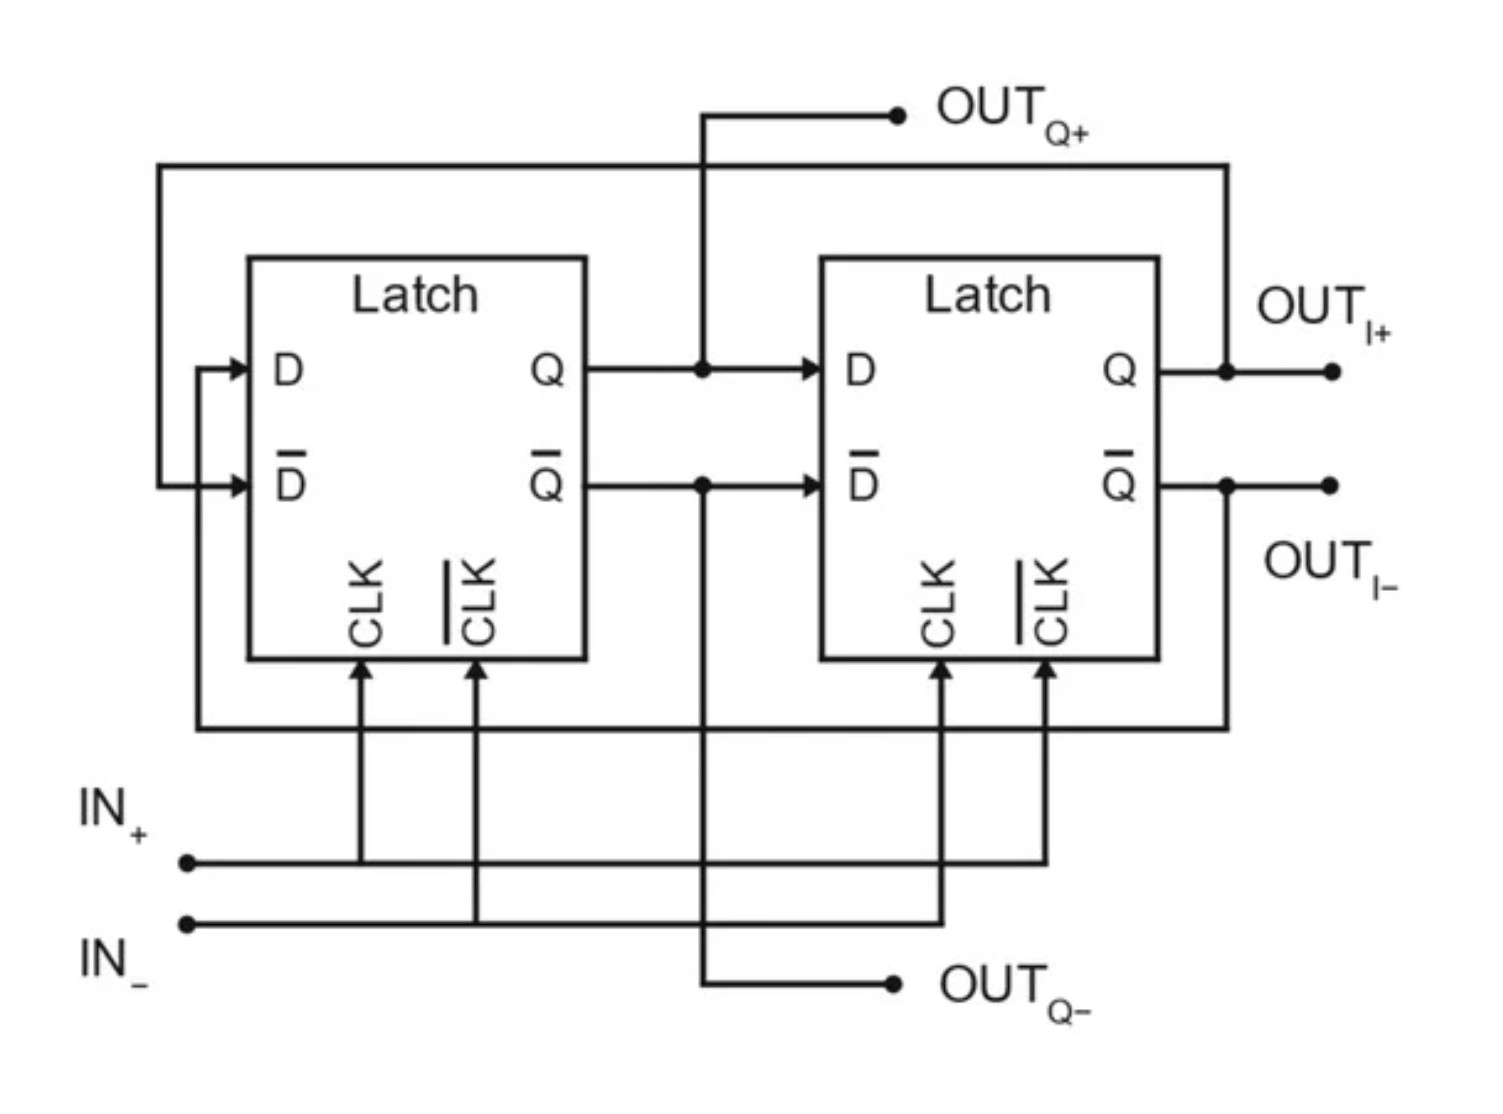
\includegraphics[width=0.8\textwidth]{IQ.jpg}
    \caption{Divider as a master–slave arrangement of two latches. IN+/IN- are the differential input signals, while OUTI+/OUTI- and OUTQ+/OUTQ- are the two quadrature differential output signals.}
    \label{fig:Wire Scaling}
\end{figure}


\subsection{Topology Selection}
The choice of a clocked tri-state inverter-based latch over alternative structures like Current Mode Logic (CML) or dynamic logic is driven by several design requirements:

\begin{itemize}
    \item \textbf{Full-Swing Operation:} The tri-state inverter provides rail-to-rail output levels, ensuring high noise immunity and eliminating the need for additional level shifters before the pulse-shaping stage.
    \item \textbf{Dynamic Power Scaling:} Power consumption is primarily dynamic, allowing for better efficiency in quarter-rate architectures where the distribution frequency is reduced to 8 GHz.
    \item \textbf{PVT Robustness:} As a static implementation, it avoids the leakage and charge-sharing issues inherent in dynamic topologies, providing a stable $90^\circ$ phase relationship across all operating corners.
\end{itemize}

\begin{figure}[H]
    \centering
    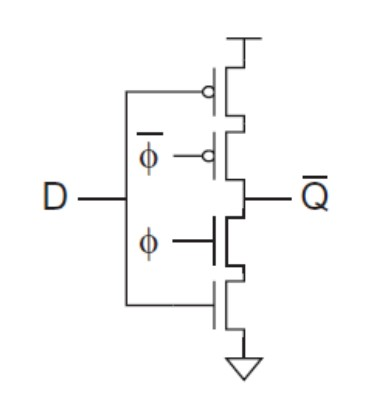
\includegraphics[width=0.7\textwidth]{c2mos.jpg}
    \caption{Clocked CMOS ($C^2MOS$).}
    \label{fig:Wire Scaling}
\end{figure}


\section{Simulation}
\subsection{Negative Latch Schematic (Clocked $C^2$MOS)}
\label{subsec:negative_latch_sim}

The fundamental building block of the IQ divider is the differential static latch, implemented here using a \textbf{Clocked CMOS ($C^2$MOS)} topology. This structure is chosen for its high-speed performance and rail-to-rail output swing.

\begin{itemize}
    \item \textbf{Input Stage:} The schematic features a clocked tri-state inverter where the input signal is gated by the differential clock signals ($\text{CLK}$ and $\text{CLKb}$). This ensures that the input is only sampled during the active phase of the clock.
    
    \item \textbf{Storage Element:} A cross-coupled inverter pair (regenerative latch) is utilized to maintain the logic state when the input stage enters a high-impedance (tri-state) mode.
    
    \item \textbf{Operation:} When the clock is active, the tri-state inverter is enabled, and the latch transparently passes the input to the output. When the clock toggles, the input stage disconnects, and the cross-coupled structure holds the previous value, providing robust static operation and immunity to leakage.
\end{itemize}

\begin{figure}[H]
    \centering
    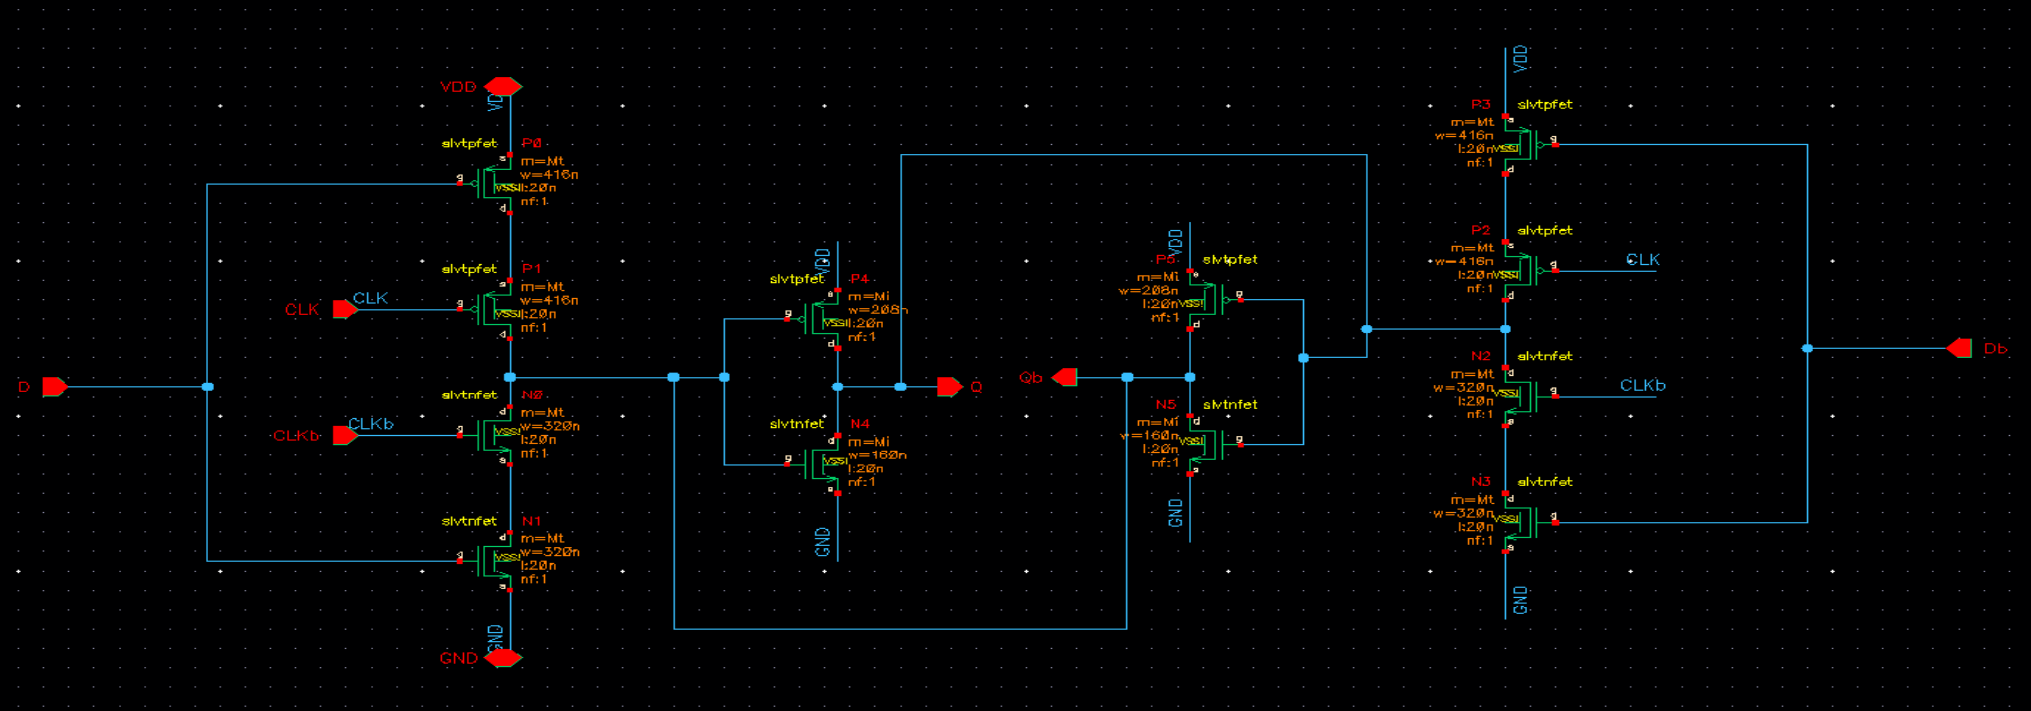
\includegraphics[width=1\textwidth]{N_latch.png}
    \caption{Negative Static Latch Schematic.}
    \label{fig:Wire Scaling}
\end{figure}

\subsection{IQ Divider System Schematic}
\label{subsec:iq_divider_system_sim}

The complete IQ divider is formed by cascading two of the previously described latches (Master and Slave) in a closed-loop configuration.

\begin{itemize}
    \item \textbf{Negative Feedback Loop:} The differential outputs of the slave latch are cross-coupled and fed back to the inputs of the master latch. This inversion in the feedback path is what enables the frequency division (divide-by-2) functionality.
    
    \item \textbf{Quadrature Phase Generation:} 
    \begin{itemize}
        \item The Master Latch triggers on the rising edge of the clock.
        \item The Slave Latch triggers on the falling edge of the clock.
        \item This $180^\circ$ difference in the high-speed clock domain results in a precise $90^\circ$ phase shift at the divided output frequency, producing the $I$ and $Q$ phases ($0^\circ, 90^\circ, 180^\circ, 270^\circ$).
    \end{itemize}
    
    \item \textbf{Simulation Setup:} The schematic is simulated with a 16 GHz differential input clock to verify the generation of stable 8 GHz quadrature outputs.
\end{itemize}

\begin{figure}[H]
    \centering
    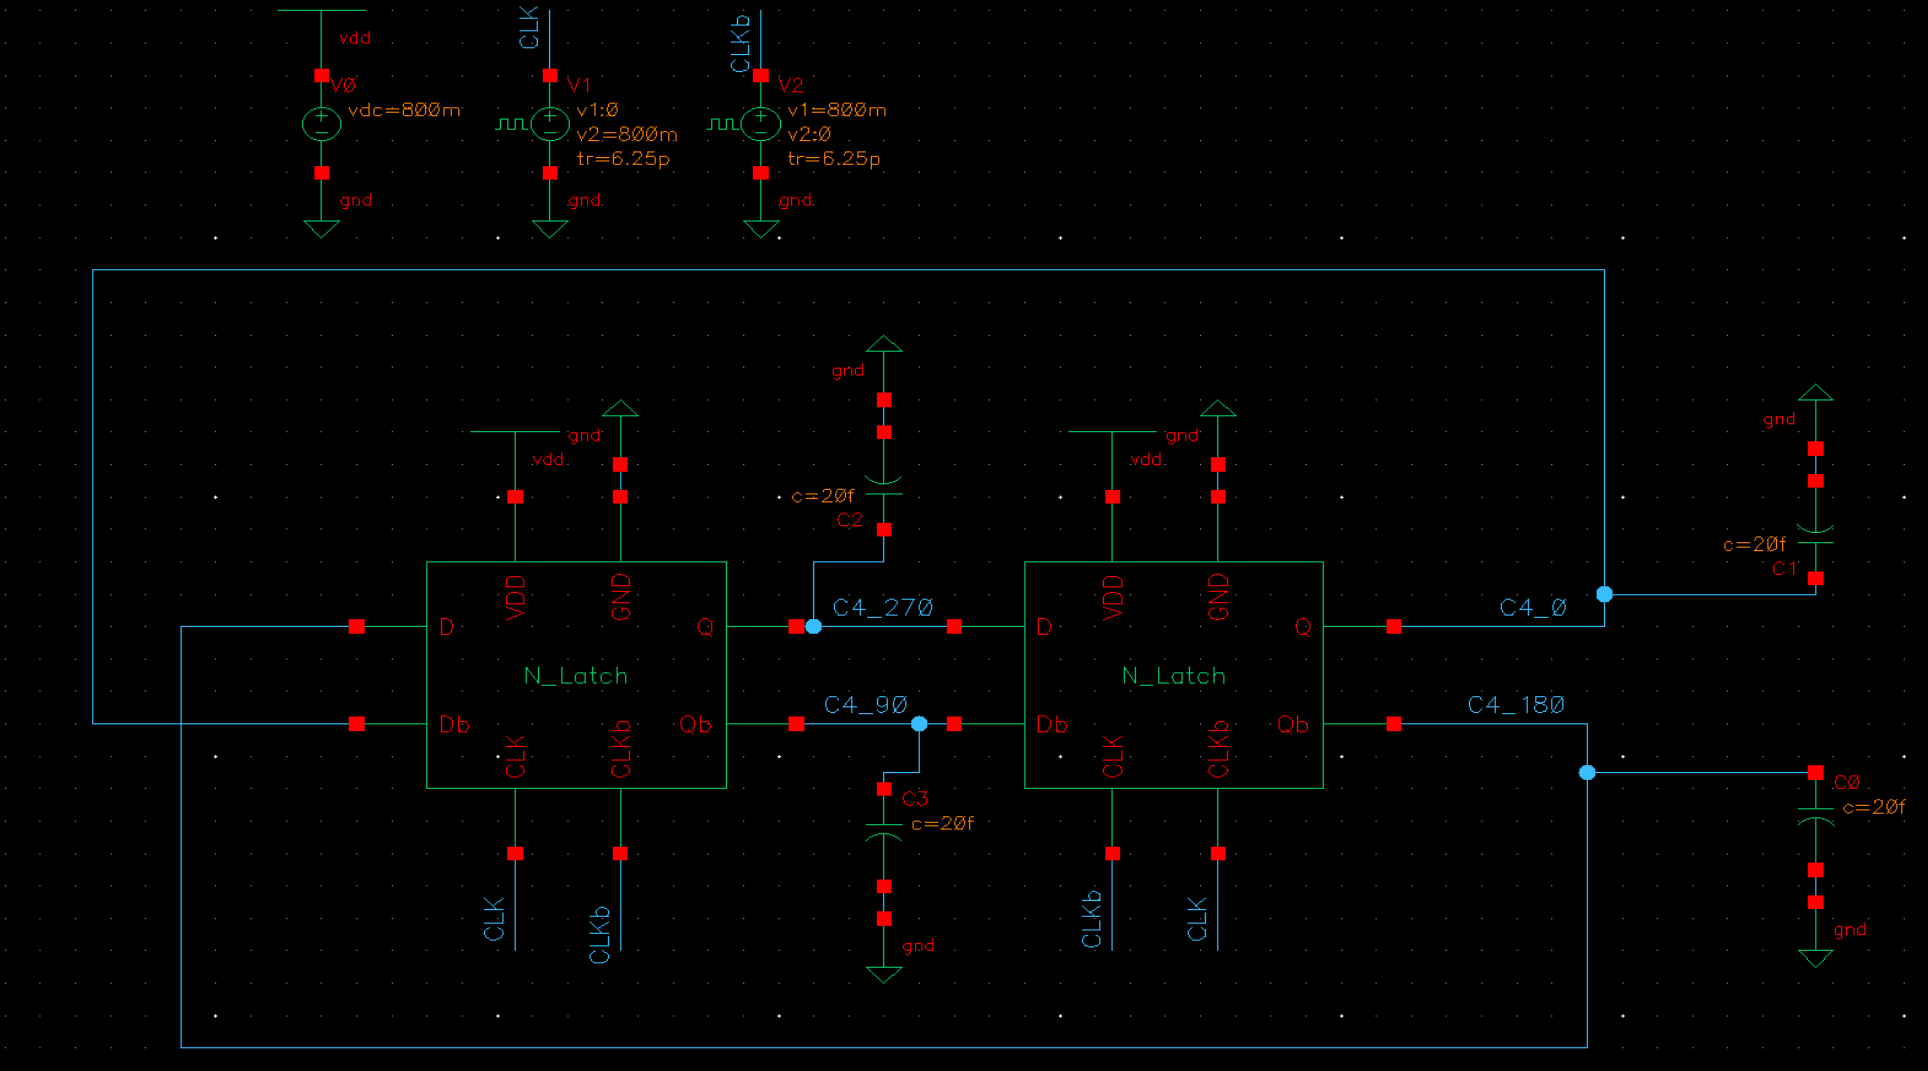
\includegraphics[width=1\textwidth]{IQ_divider.png}
    \caption{I/Q Divider Schematic.}
    \label{fig:Wire Scaling}
\end{figure}

\subsection{Transient Response Analysis}
\label{subsec:transient_analysis}

The transient simulation results verify the functional operation of the IQ divider, specifically its ability to perform frequency division and generate accurate quadrature phases.

\begin{itemize}
    \item \textbf{Frequency Division and Scaling:} The top two traces show the differential input clocks ($CLK$ and $CLKb$) operating at the high-speed PLL\ frequency of 16~GHz. The four output traces ($C4\_0$ through $C4\_270$) operate at exactly half that frequency (8~GHz), confirming the successful divide-by-2 operation required for a quarter-rate clocking system.
    
    \item \textbf{Quadrature Phase Generation:} The simulation confirms the $90^\circ$ phase relationship between the outputs. By observing the simulation markers, it is evident that the $90^\circ$ phase ($C4\_90$) is shifted by half a clock cycle of the 16~GHz input relative to the $0^\circ$ phase ($C4\_0$). This equates to exactly one-quarter of the 8~GHz output period ($T/4$).
    
    \item \textbf{Timing Accuracy:} The crossing points of the quadrature phases align precisely with the 400~mV common-mode level (indicated by horizontal markers H1, H2, H3, and H4). The symmetry observed in the rising and falling edges indicates low internal Duty Cycle Distortion (DCD) within the divider circuit itself.
\end{itemize}

\begin{figure}[H]
    \centering
    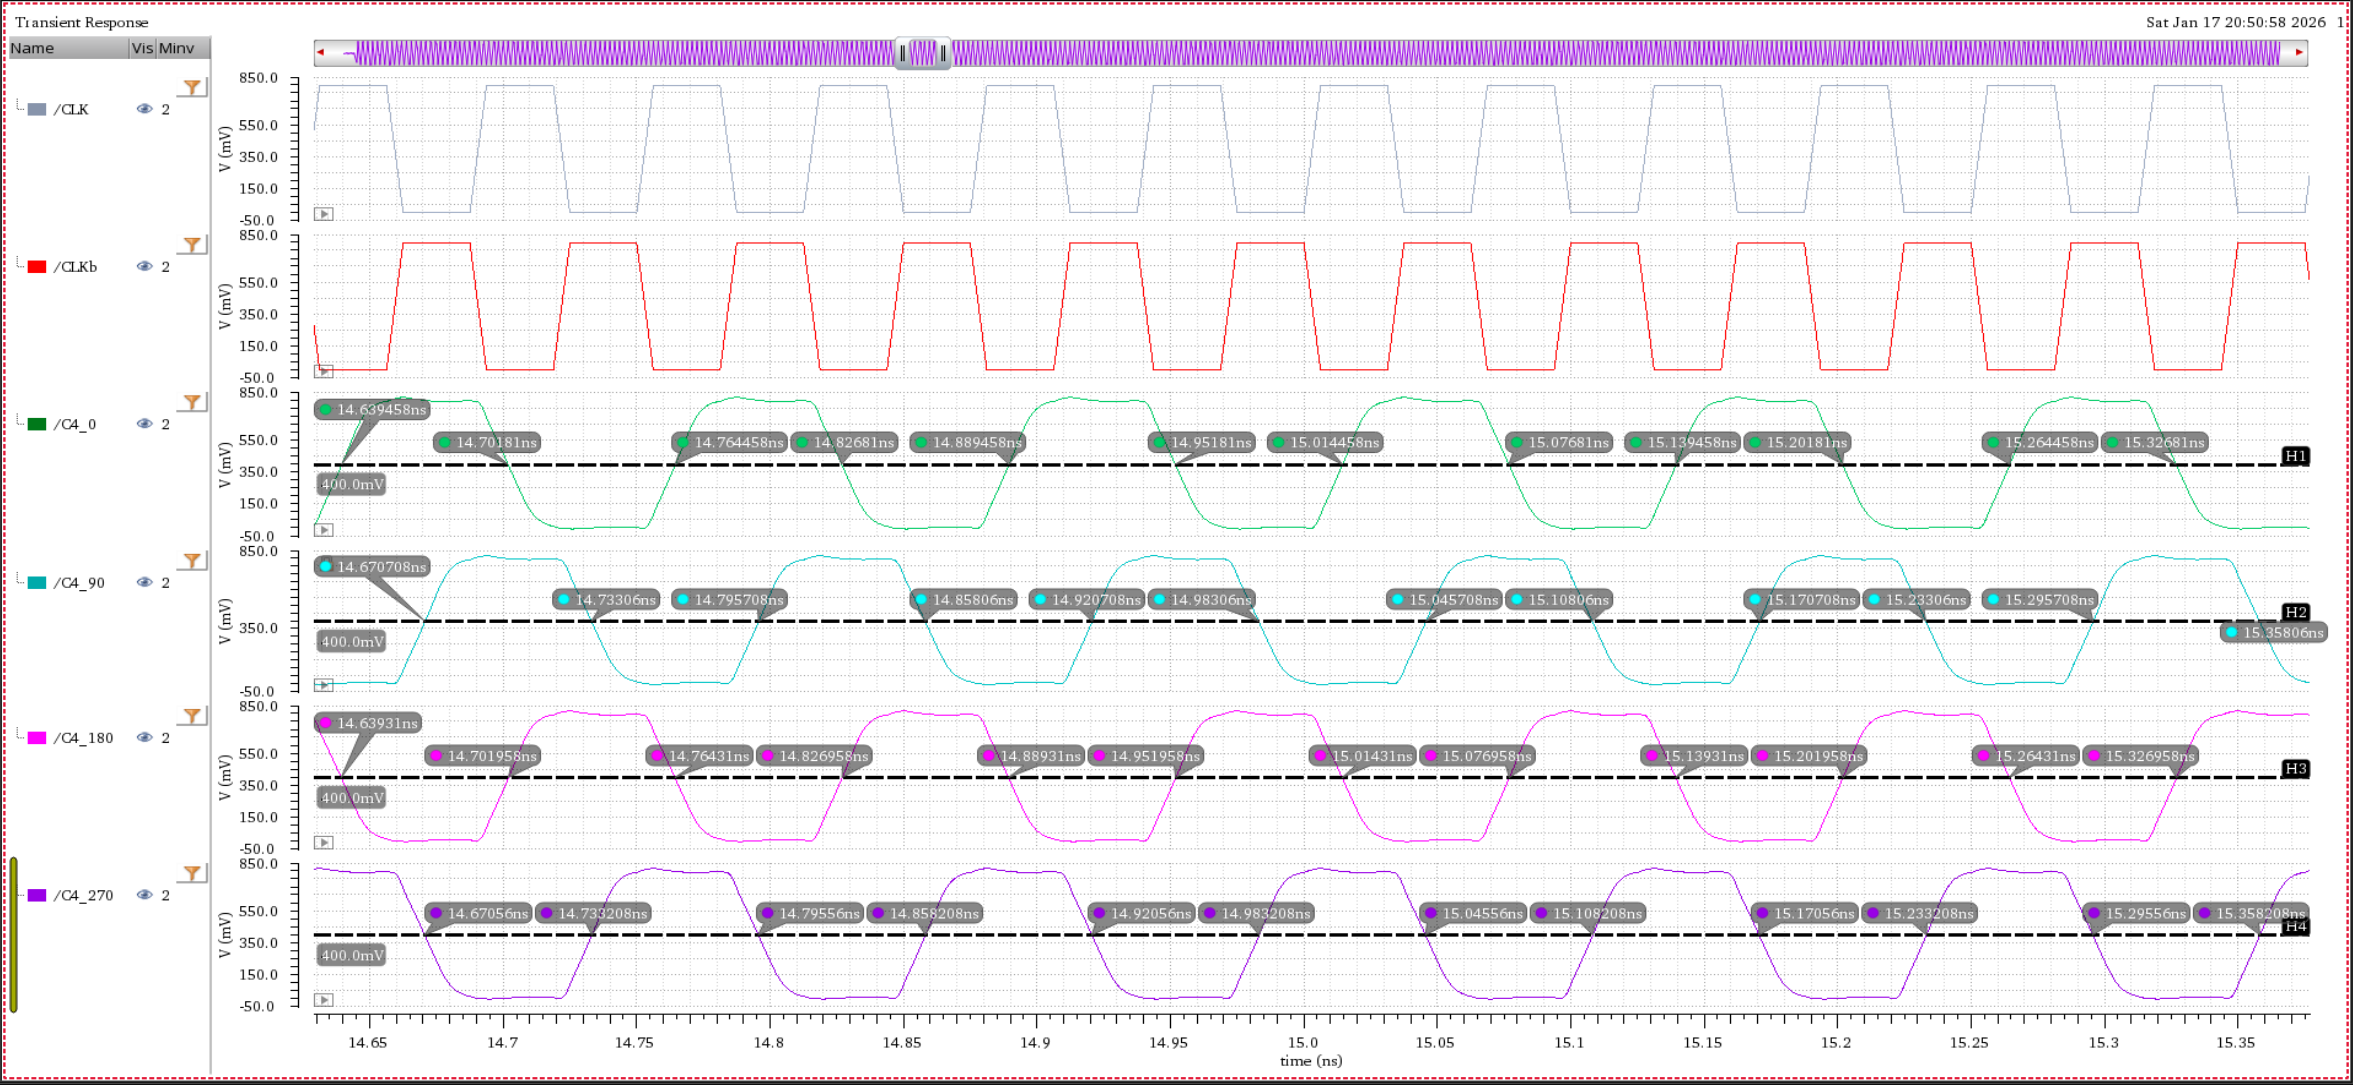
\includegraphics[width=1\textwidth]{Transient.png}
    \caption{Transient simulation waveforms of the IQ Divider showing the 16~GHz input clock and the generated 8~GHz quadrature phases ($I/Q$).}
    \label{fig:Wire Scaling}
\end{figure}

\section{Simulation Methodology: PSS Engine Selection}
To characterize the I/Q Divider and Pulse Shaper, Periodic Steady State (PSS) analysis was utilized. Selecting the correct simulation engine is critical for ensuring convergence in circuits operating at 16~GHz.

\subsection{Shooting Newton Engine}
The Shooting Newton engine is a time-domain method that iteratively solves for the periodic steady-state solution. This engine is particularly effective for:
\begin{itemize}
    \item \textbf{High Non-linearity:} Circuits that switch abruptly between supply rails.
    \item \textbf{Sharp Edges:} Handling the fast sways and high-frequency transients of the 8~GHz quadrature pulses.
\end{itemize}
For this thesis, the Shooting engine was selected as the primary solver because the frequency divider's master-slave latch topology exhibits digital-like switching behavior that is difficult to represent accurately in the frequency domain.

\subsection{Harmonic Balance Engine}
Harmonic Balance (HB) is a frequency-domain solver that represents signals as a sum of harmonics. While HB is highly efficient for sinusoidal signals and high-Q LC oscillators, it is less suited for this specific implementation. Representing a 25\% duty cycle pulse at 8~GHz would require a prohibitive number of harmonics to capture the sharp transition edges, leading to increased simulation time and reduced numerical stability.

\begin{table}[H]
\centering
\caption{Comparison of PSS Simulation Engines}
\label{tab:pss_engines}
\begin{tabular}{@{}lll@{}}
\toprule
\textbf{Feature} & \textbf{Shooting Newton} & \textbf{Harmonic Balance} \\ \midrule
Domain           & Time Domain              & Frequency Domain          \\
Signal Type      & Square/Pulse Waves       & Sinusoidal/Narrowband     \\
Non-linearity    & High (Switching)         & Mild (Analog)             \\
Best for         & Dividers, Ring OSCs      & LC-VCOs, LNAs             \\ \bottomrule
\end{tabular}
\end{table}

\subsection{Beat Frequency ($f_{beat}$)}
The beat frequency was established at \textbf{8~GHz}. This choice is dictated by the fact that 8~GHz is the greatest common divisor of the input (16~GHz) and the quadrature output (8~GHz). Setting $f_{beat} = 8$~GHz ensures the simulator evaluates the circuit over a 125~ps fundamental period, which is the minimum time required to capture one full cycle of the output and two full cycles of the input reference.

\subsection{Number of Harmonics}
The number of harmonics was set to \textbf{30}. This parameter defines the spectral range of the simulation, providing coverage up to 240~GHz ($30 \times 8$~GHz). This high count is necessary for two reasons:
\begin{itemize}
    \item \textbf{Waveform Integrity:} It provides sufficient resolution to reconstruct the sharp transition edges preventing errors in the calculated rise/fall times.
    \item \textbf{Noise Folding:} In the subsequent Pnoise analysis, a larger number of harmonics allows the simulator to accurately account for high-frequency noise folding, which is essential for a precise estimation of the random jitter ($R_j$).
\end{itemize}

\begin{figure}[H]
    \centering
    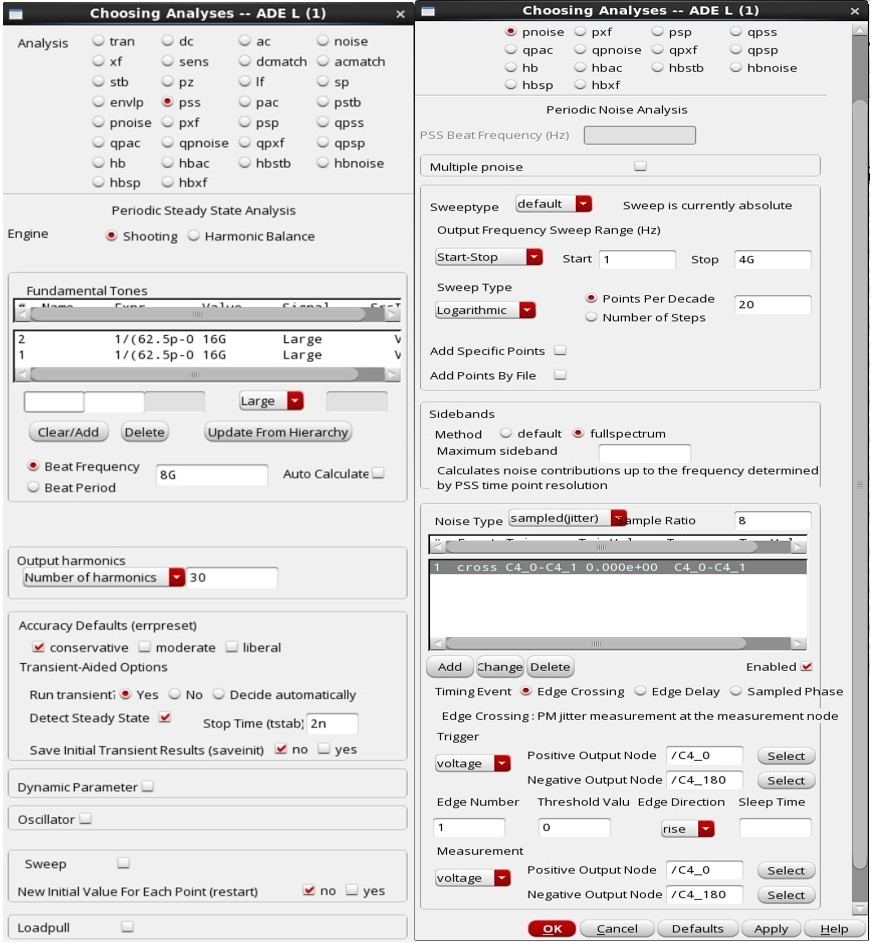
\includegraphics[width=0.6\textwidth]{PSS&Pnoise.jpg}
    \caption{Periodic Steady State (PSS)/ Pnoise Simulation Tab Options.}
    \label{fig:Wire Scaling}
\end{figure}

\subsubsection{Jitter Simulation Results}



\begin{figure}[H]
    \centering
    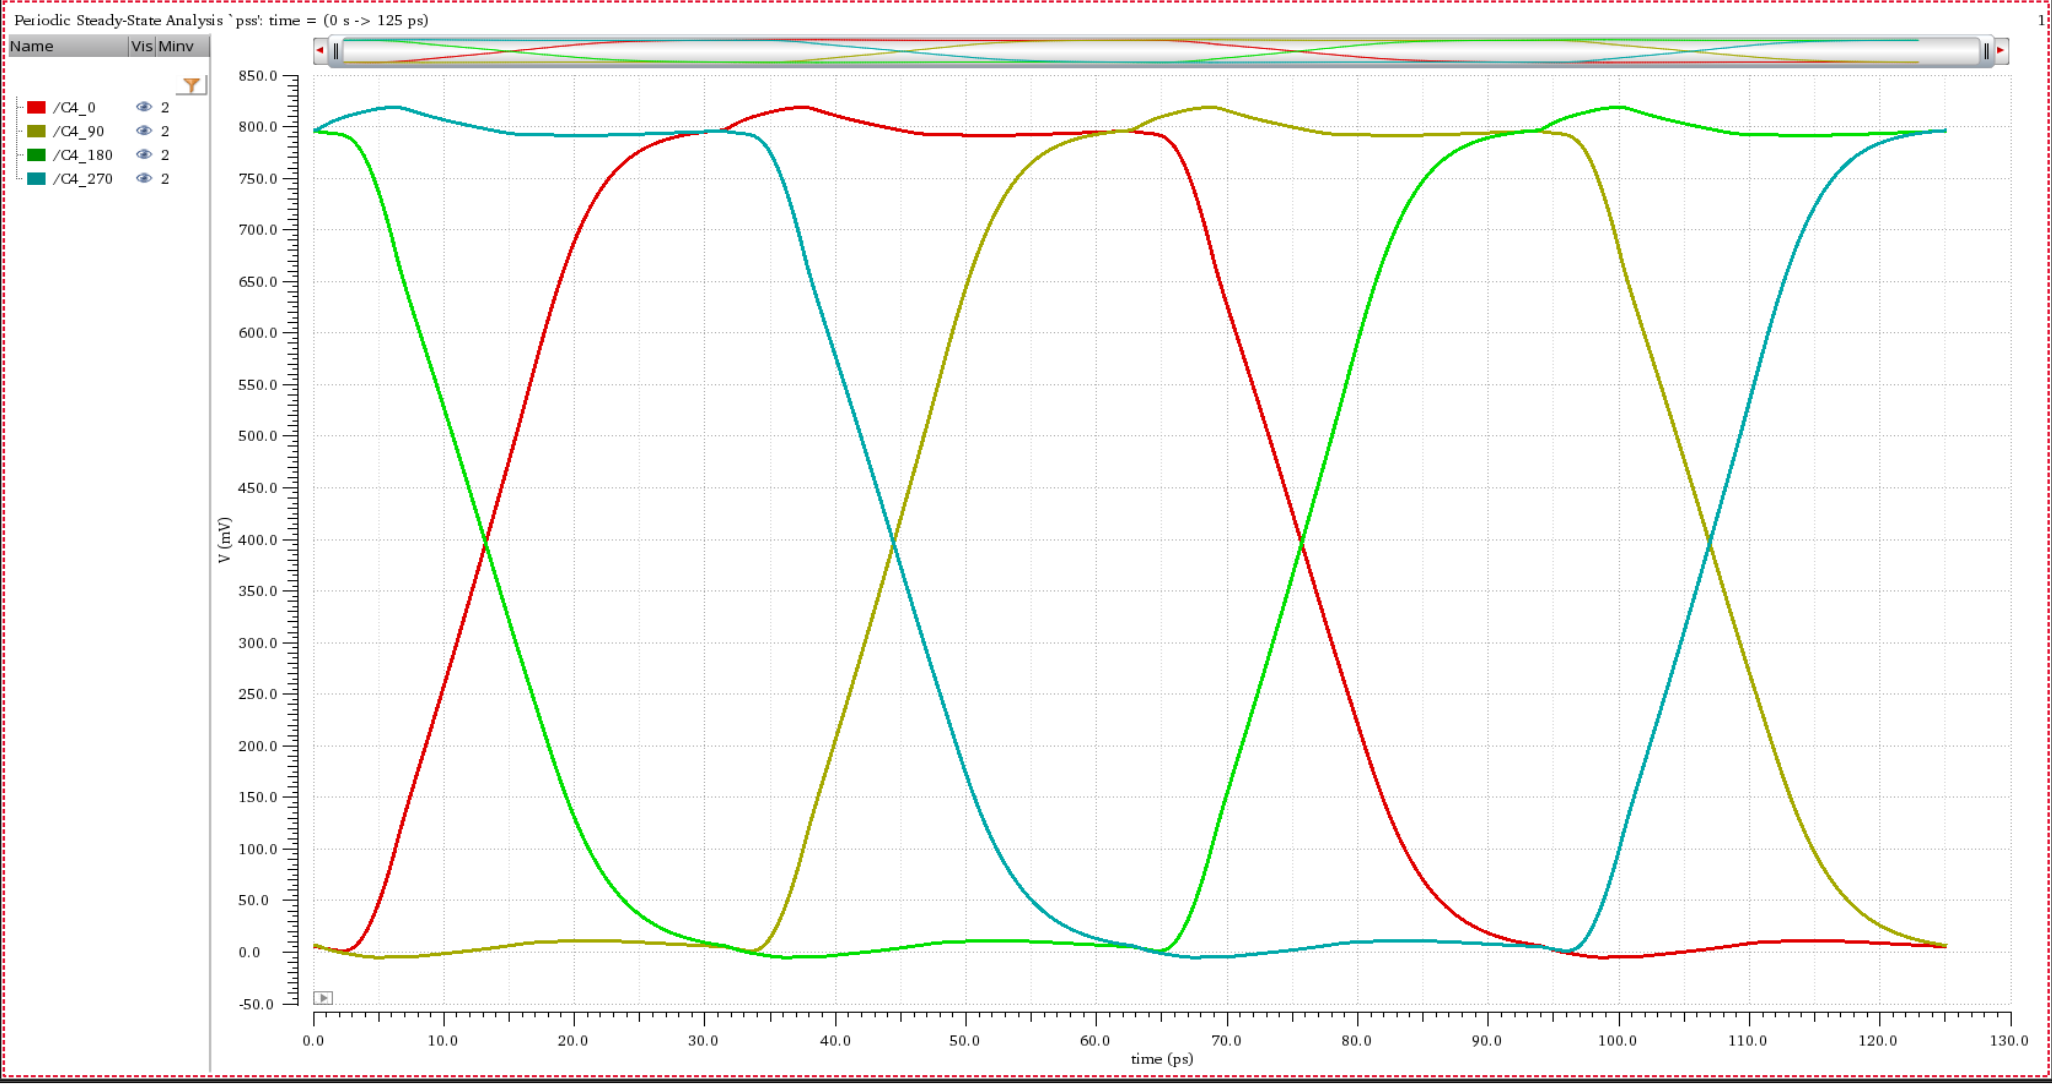
\includegraphics[width=0.8\textwidth]{Pssr.png}
    \caption{PSS Simulation Result.}
    \label{fig:Wire Scaling}
\end{figure}

\begin{figure}[H]
    \centering
    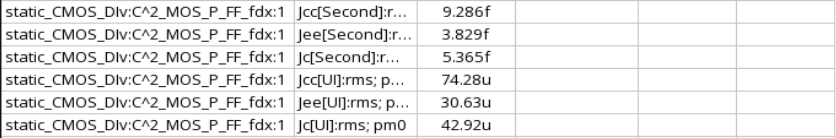
\includegraphics[width=0.8\textwidth]{RJr.png}
    \caption{Random Jitter Results.}
    \label{fig:Wire Scaling}
\end{figure}

\begin{figure}[H]
    \centering
    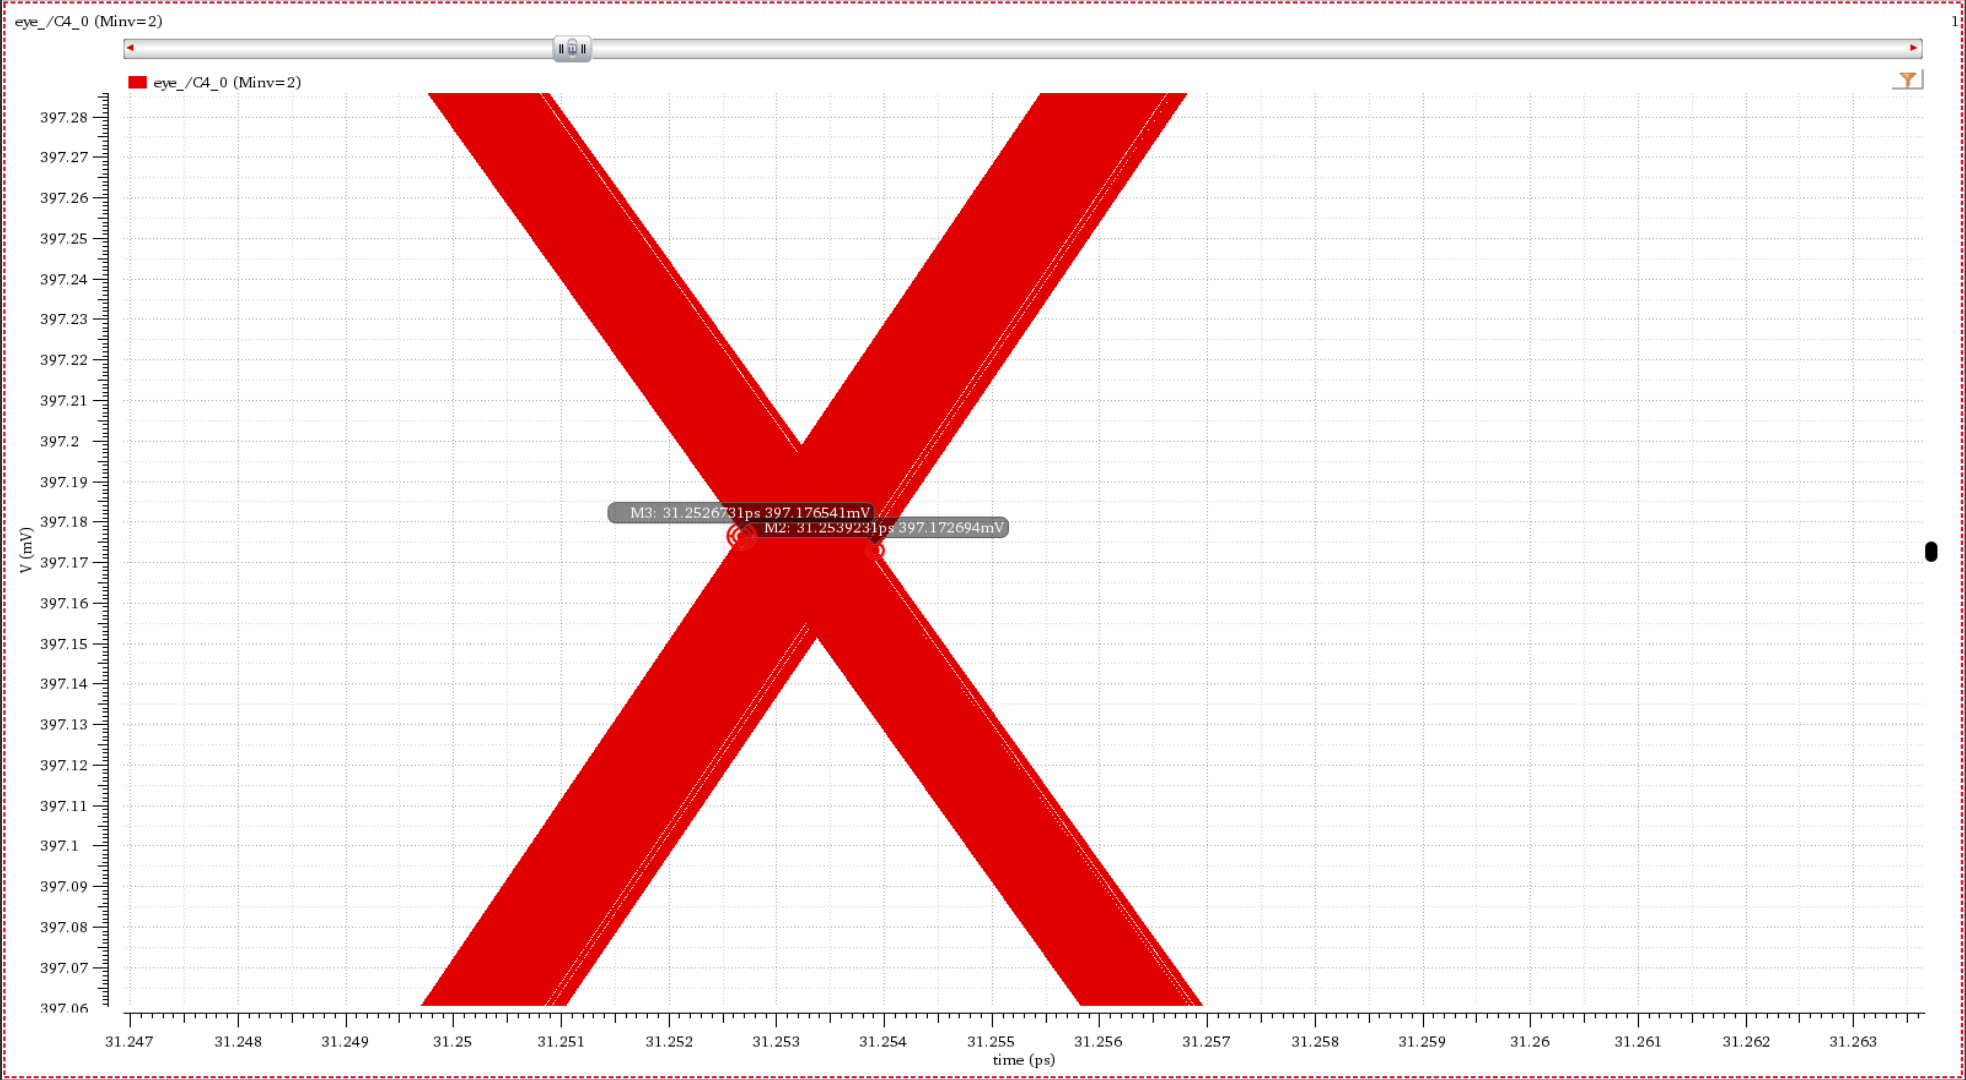
\includegraphics[width=0.8\textwidth]{Djr.png}
    \caption{Determinstic Jitter Results.}
    \label{fig:Wire Scaling}
\end{figure}





\section{High speed Mux}
% ==================================================
% 3.1.1 TOPOLOGY A: TRANSMISSION GATE
% ==================================================
\subsection{Topology A: Transmission Gate (TG) Implementation}
\label{subsec:tg_impl}

The first topology evaluated is the Transmission Gate (TG) multiplexer. This architecture is historically significant for its simplicity and zero static power consumption. In this implementation, the conventional tree structure was flattened into a single-stage 4:1 multiplexer to align with the unified Quarter-Rate architecture.

\subsubsection{Circuit Implementation}
The circuit consists of four parallel switches connecting the four data inputs ($D_0-D_3$) to a common output node ($V_{out}$).
\begin{itemize}
    \item \textbf{Switch Structure:} Each switch is implemented as a Complementary CMOS Transmission Gate, consisting of an NMOS and a PMOS transistor in parallel.
    \item \textbf{Control Logic:} The gates of these transistors are driven by the 25\% duty cycle clock phases ($\Phi$ and $\overline{\Phi}$). When a clock phase is active (High), both transistors turn ON, creating a low-impedance path for the data to pass to the output.
    
\end{itemize}

\begin{figure}[H]
    \centering
    % REPLACE 'piso.jpg' with your filename
    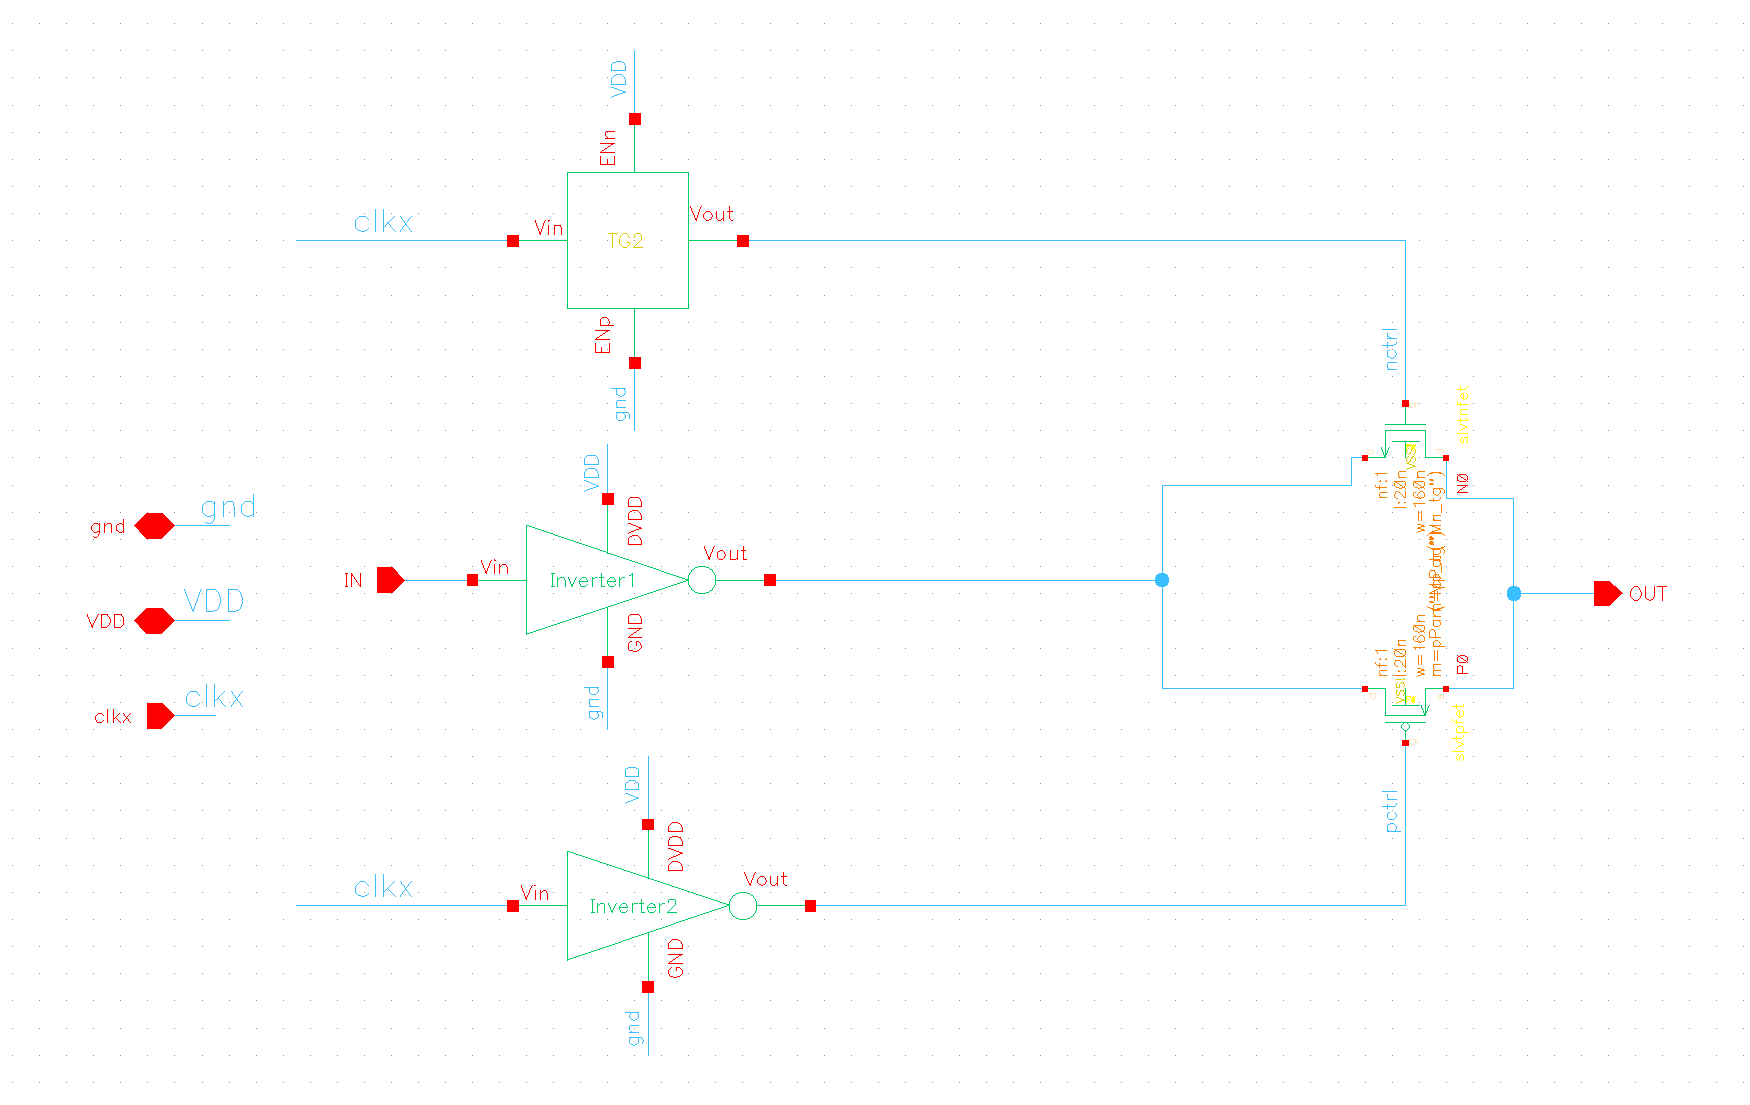
\includegraphics[width=0.8\textwidth]{tgslice (2).png}
    \caption{Schematic implementation of a single Slice within the Quarter-Rate Transmission Gate (TG) multiplexer. The central TG switch is driven by the 25\% duty cycle clock phase ($clkx$) and its complement to enable the data path ($IN \rightarrow OUT$) for exactly 1 UI.}
    \label{fig:tgslice_schematic}
\end{figure}

\subsubsection{Sizing Strategy (Resistance vs. Capacitance)}
The performance of the TG topology is governed by the RC time constant at the output node. The optimization goal was to minimize this time constant ($\tau = R_{on} \times C_{total}$) to maximize the bandwidth.
\begin{itemize}
    \item \textbf{Design Variable:} A parametric sweep of the transistor Multiplier ($M$) was performed, maintaining a fixed PMOS-to-NMOS width ratio which comes from the mobility ratio of NMOS and Pmos ($W_p$=1.6*$W_n$).
    \item \textbf{Trade-off Analysis:} Increasing the Multiplier of the transistor both PMOS and NMOS ($M$) reduces the On-Resistance ($R_{on}$) of the switch, which theoretically increases bandwidth. However, increasing width simultaneously increases the parasitic diffusion capacitance ($C_{diff}$) contributed by the switch to the output node.
    
    \item \textbf{Delay Matching (TG vs. Inverter):} A critical design feature is the inclusion of the Transmission Gate in the PMOS control path. Since the NMOS path uses an Inverter (which adds propagation delay), the TG is inserted in the PMOS path to replicate this delay. This ensures that the drive signals arrive at the gates of output PMOS and NMOS simultaneously, minimizing crossover current and skew.
\end{itemize}


\subsubsection{Simulation Results: Transient Response and Eye Diagram}
The functional verification of the Transmission Gate (TG) topology was performed at a data rate of 64 Gb/s. The simulation results confirm that the 25\% duty cycle clocking scheme effectively prevents contention and allows for correct serialization of the parallel input data.

\begin{figure}[htbp]
    \centering
    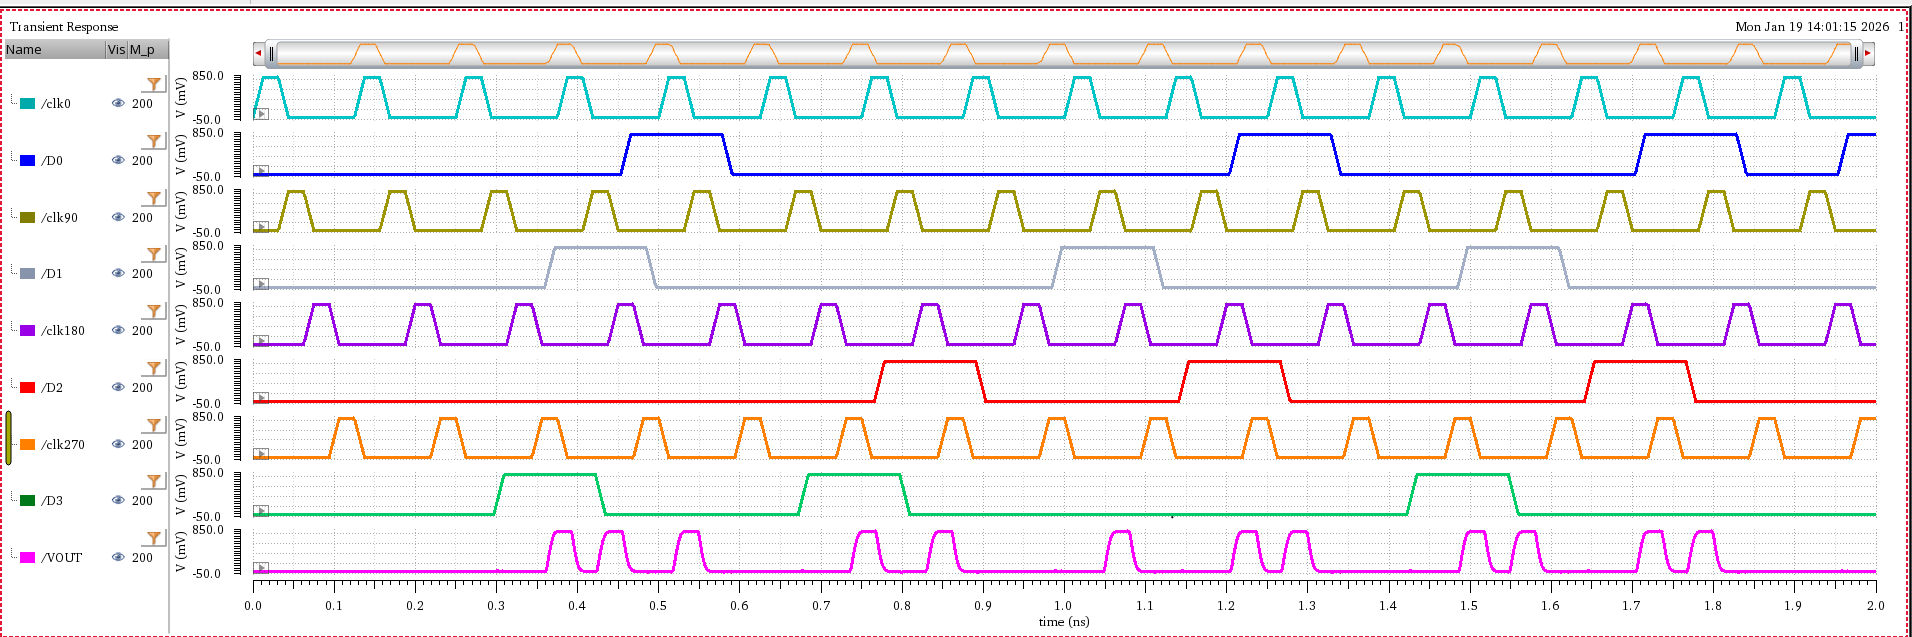
\includegraphics[width=0.8\textwidth]{tgout_2n.png}
    \caption{Transient response of the Transmission Gate multiplexer output at 64 Gb/s. The waveform demonstrates the correct sequential selection of the input bits ($D_0-D_3$).}
    \label{fig:tg_transient}
\end{figure}

Figure \ref{fig:tg_transient} illustrates the large-signal transient response. The output waveform follows the input data pattern, validating the timing logic of the transmission gates.

\begin{figure}[htbp]
    \centering
    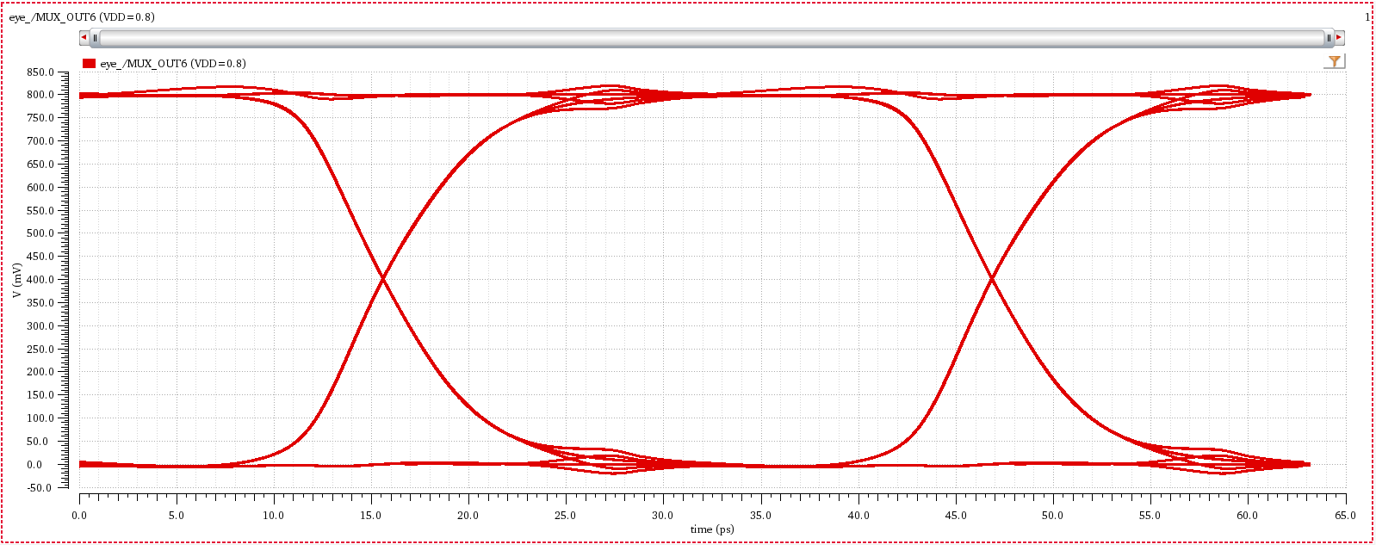
\includegraphics[width=0.8\textwidth]{tgeye.png}
    \caption{Simulated Eye Diagram of the Transmission Gate topology at 64 Gb/s.}
    \label{fig:tg_eye}
\end{figure}

Figure \ref{fig:tg_eye} presents the eye diagram captured at the output node. The simulation confirms that the Transmission Gate topology is capable of driving the load with a visible eye opening, successfully operating at the target data rate but with observed Intersymbol interference.

\begin{figure}[H]
    \centering
    % --- First Subfigure (Deterministic Jitter) ---
    \begin{subfigure}[b]{0.6\textwidth}
        \centering
        % Replace 'image_deterministic.png' with your actual filename
        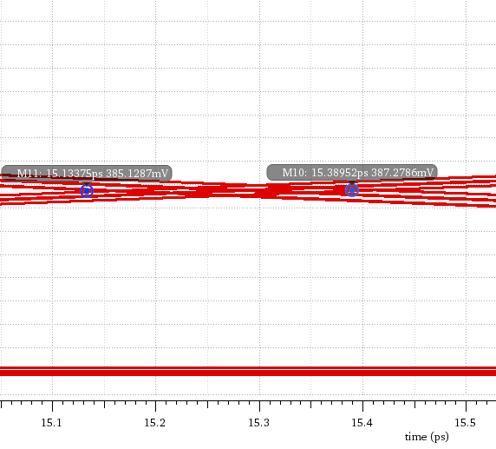
\includegraphics[width=\textwidth]{tg deterministic.png}
        \caption{Deterministic Jitter with clean supply}
        \label{fig:dj_zoom}
    \end{subfigure}
    \hfill % Adds flexible space between the images
    % --- Second Subfigure (Total Jitter) ---
    \begin{subfigure}[b]{0.6\textwidth}
        \centering
        % Replace 'image_total.png' with your actual filename
        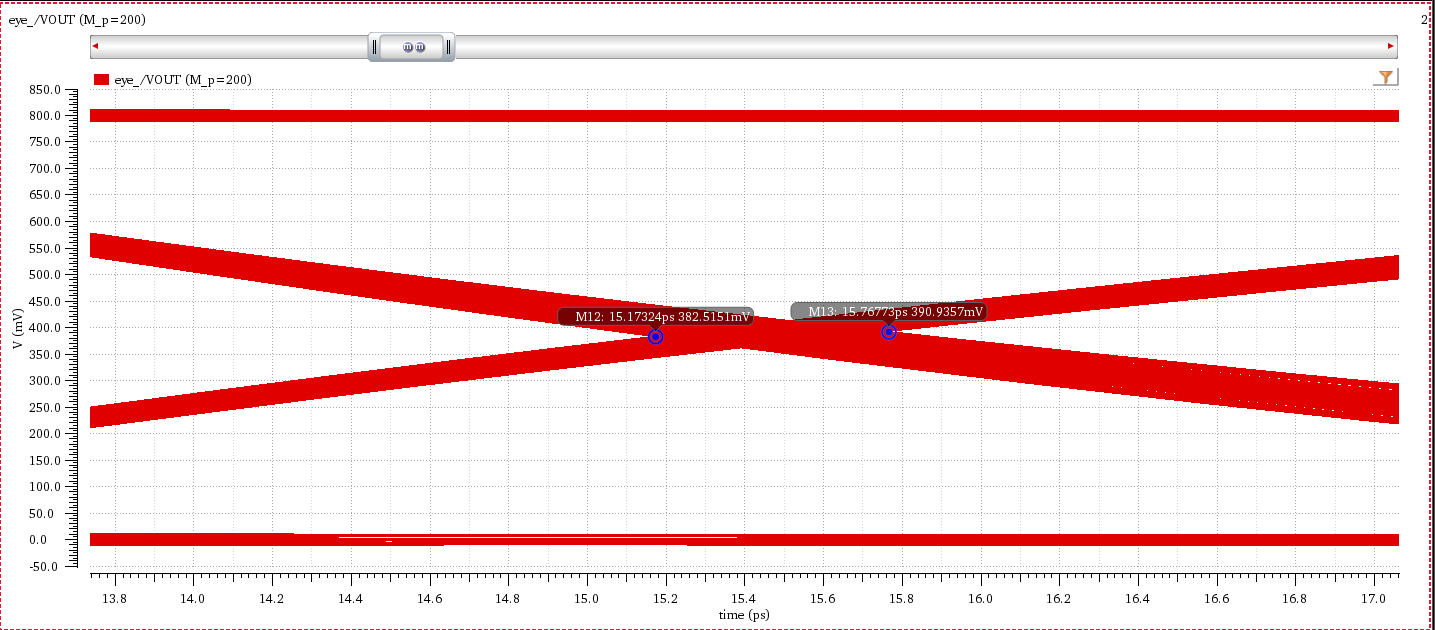
\includegraphics[width=\textwidth]{tg psij.png}
        \caption{Total Jitter with noisy supply}
        \label{fig:tj_zoom}
    \end{subfigure}
    
    \caption{Jitter measurement comparison showing (a) Deterministic Jitter components and (b) Total Jitter accumulation.}
    \label{fig:jitter_comparison}
\end{figure}
% ==================================================
% TG SIMULATION METRICS SUMMARY (SCHEMATIC LEVEL)
% ==================================================
\subsubsection{Simulation Metrics Summary}
\label{subsubsec:tg_sim_metrics}

\begin{table}[H]
    \centering
    \caption{Summary of Simulated Performance Metrics for the Transmission Gate Topology (Schematic Level)}
    \label{tab:tg_metrics}
    \renewcommand{\arraystretch}{1.4} % Adds vertical spacing to rows
    \setlength{\tabcolsep}{12pt}      % Adds horizontal spacing to columns
    \begin{tabular}{|l|c|}
        \hline
        \textbf{Specification} & \textbf{Value} \\ \hline
        \textbf{Power (mW)} & 5.883 \\ \hline
        \textbf{Swing (mV)} & 799.8 \\ \hline
        \textbf{Eye width (ps)} & 30.66 \\ \hline
        \textbf{Eye Crossing (mV)} & 387.255 \\ \hline
        \textbf{Deterministic Jitter (fs)} & 255.77 \\ \hline
        \textbf{Power Supply Induced Jitter (fs)} & 185.59 \\ \hline
        \textbf{Total Jitter (fs)} & 441.36 \\ \hline
        \textbf{Eye rise time (ps)} & 8 \\ \hline
        \textbf{Eye fall time (ps)} & 8 \\ \hline
    \end{tabular}
\end{table}

The metrics in Table \ref{tab:tg_metrics} demonstrate that the Transmission Gate topology, when implemented with the proposed 25\% duty cycle clocking at the schematic level, achieves good signal integrity and rail-to-rail output swing it provides a full output swing of 799.1 mV, maximizing the Signal-to-Noise Ratio (SNR)..

The results in Table \ref{tab:tg_metrics} reveal a critical trade-off regarding power consumption. Although the Transmission Gate topology theoretically consumes zero static power, the recorded power consumption of 5.883 mW is significant.. 

To meet the strict bandwidth requirements and reduce signal attenuation, the switches had to be sized with extremely large widths ($W$) to minimize their on-resistance ($R_{on}$). However, this large size introduces a massive parasitic gate capacitance ($C_{gg}$) that the clock distribution network must drive. Consequently, the power figure shown is almost entirely **dynamic switching power** ($P \propto C_{gg} V^2 f$) dissipated by the pre-drivers charging and discharging these large capacitive loads at 32 GHz.

\subsection{Topology B: Pseudo-CML (Resistive Load) Implementation}
\label{subsec:cml_impl}

The second topology evaluated is the Pseudo-Current Mode Logic (Pseudo-CML) driver. While traditional CML relies on a differential pair with a constant tail current, this implementation utilizes a grounded-source, resistive-load topology (often referred to as Pseudo-NMOS in high-speed I/O). This architecture was selected to overcome the voltage headroom limitations of the 22nm FD-SOI process due to the limited supply, eliminating the tail current source to maximize voltage swing at low supply voltages.

\subsubsection{Circuit Implementation}
The circuit functions as a single slice of the Quarter-Rate transmitter, consisting of a digital pre-driver stage and an analog resistive-load output stage.
\begin{itemize}
    \item \textbf{Switch Structure:} The driver utilizes a single NMOS transistor with its source grounded and its drain connected to the supply ($V_{DD}$) through a passive load resistor ($R$).
    \item \textbf{Control Logic:} The gate of the NMOS is driven by a 2-input AND gate. This gate combines the data input ($D_0$) with the sampling clock ($CLK_0$).
    \item \textbf{Pulse Carving Operation:} Since the input data ($D_0$) is stable for 4 Unit Intervals (UI), the AND gate performs a \textbf{Pulse Carving} function. It gates the static data with the 1 UI clock pulse, effectively generating a valid output signal only during the active clock phase.
    \item \textbf{Logic Operation:} The circuit operates as an inverting driver with a "Return-to-One" reset state. When the clock is Low, the NMOS is forced OFF, pulling the output High ($V_{DD}$). When the clock is High, the output follows the inverse of the data (Logic '1' turns the NMOS ON, pulling the output Low).
\end{itemize}

\begin{figure}[H]
    \centering
    % REPLACE 'cml_slice.png' with your filename
    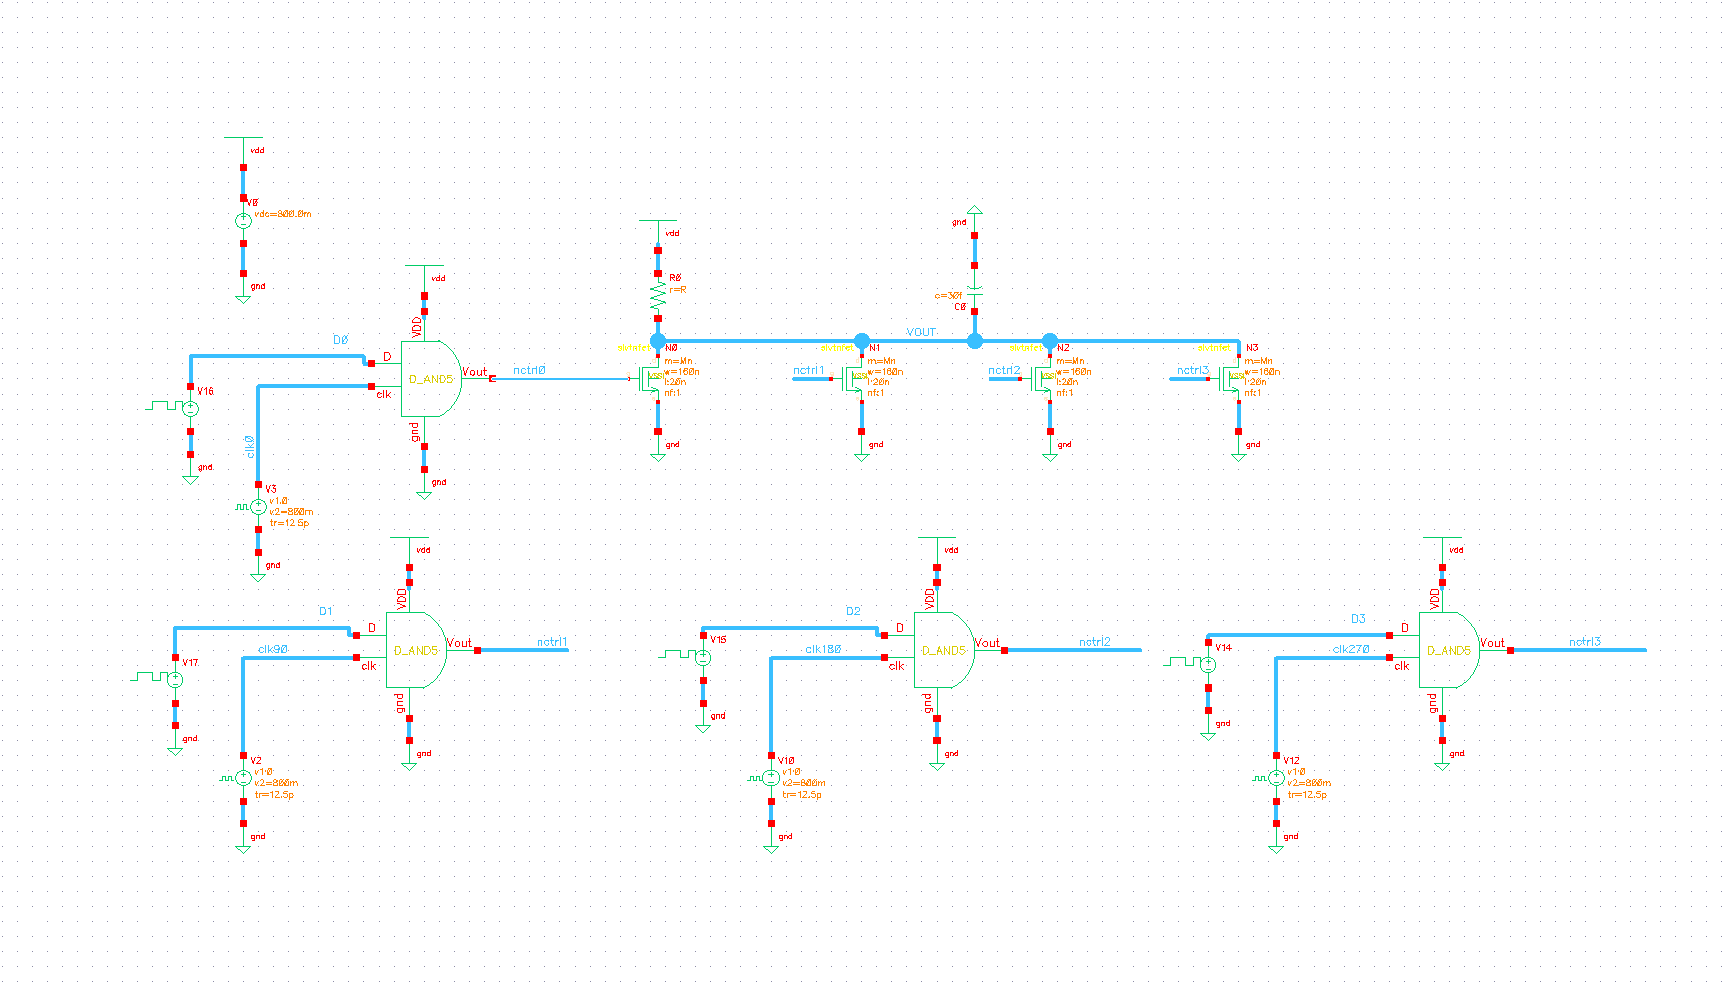
\includegraphics[width=0.8\textwidth]{Cml.png}
    \caption{Schematic implementation of a  Pseudo-CML 4-1 MUX. The circuit utilizes a resistive load and a grounded-source NMOS to maximize headroom. The AND gate performs the .}
    \label{fig:cmlslice_schematic}
\end{figure}

\subsubsection{Sizing Strategy (Rise/Fall Time Matching)}
The sizing strategy for the Pseudo-CML driver prioritized edge-rate symmetry to minimize Inter-Symbol Interference (ISI). The design procedure was decoupled into two steps based on the dominant time constants for the rising and falling edges.

\begin{itemize}
    \item \textbf{Step 1: Load Resistor Sizing (Rise Time):} Since the rising edge is passive (pull-up via $R$), the rise time is determined strictly by the $RC$ time constant at the output node. The resistor value ($R$) was calculated first to achieve a specific target rise time compatible with the 64 Gb/s data rate ($t_{rise} \approx 2.2 \cdot R \cdot C_{load}$).
    \item \textbf{Step 2: NMOS Sizing (Fall Time vs. $V_{OL}$):} The falling edge is actively driven by the NMOS transistor. The width ($W$) of the NMOS was sized to achieve an on-resistance ($R_{on}$) that yields a fall time approximately equal to the rise time calculated in Step 1.
    \item \textbf{Constraint Check ($V_{OL}$):} While matching the fall time, the design was simultaneously constrained by the minimum output voltage ($V_{out,min}$). The final $R_{on}$ had to ensure that the voltage divider formed with $R$ provided a sufficiently low $V_{OL}$ to meet the swing requirements:
    $$ V_{OL} = V_{DD} \cdot \frac{R_{on}}{R_{on} + R} $$
\end{itemize}

\subsubsection{Simulation Results: Transient Response and Eye Diagram}
The functional verification of the Pseudo-CML topology was performed at a data rate of 64 Gb/s. The simulation results demonstrate the inverting behavior.

\begin{figure}[htbp]
    \centering
    % REPLACE 'cmlout.png' with your filename
    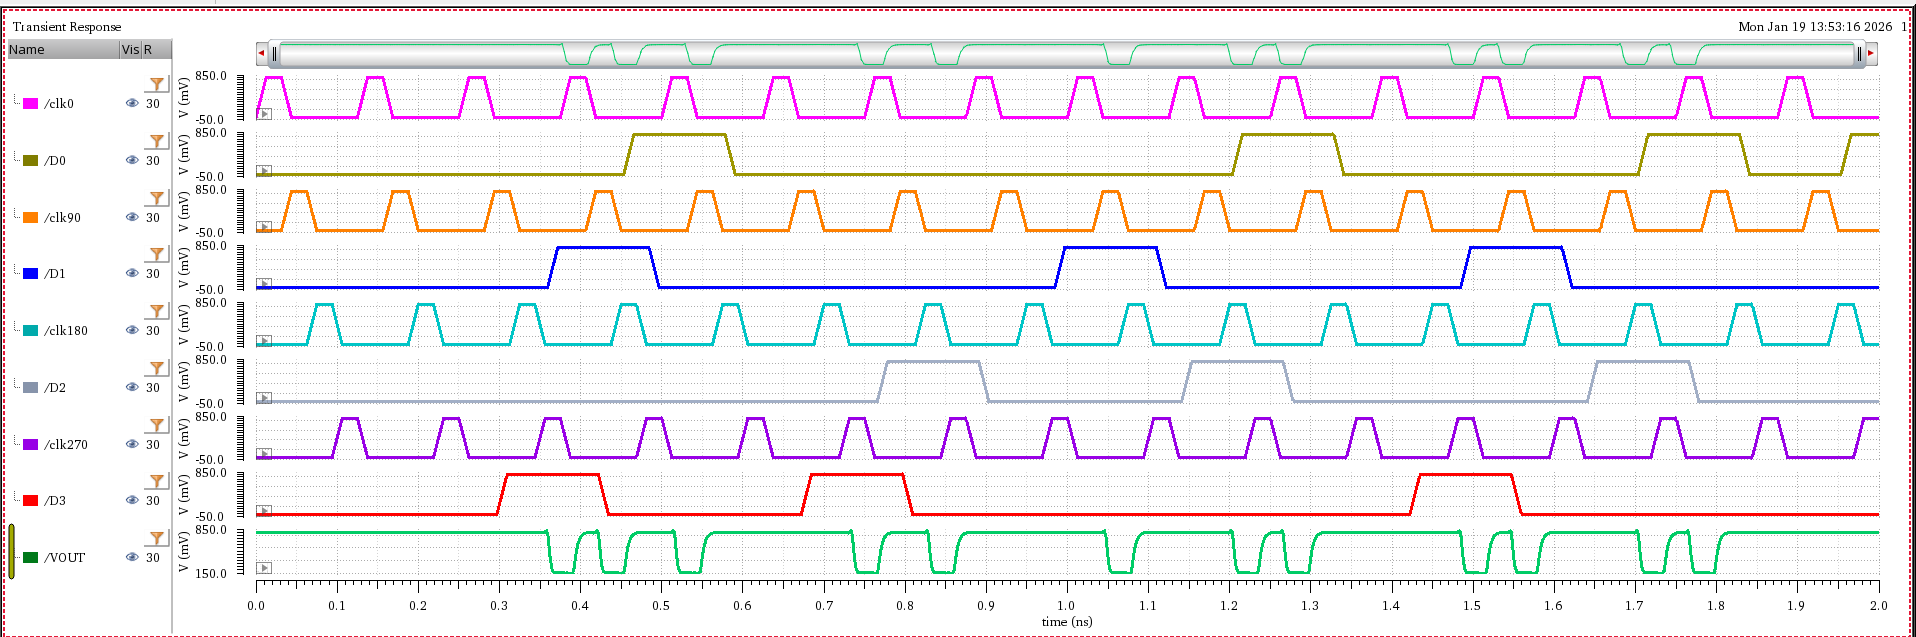
\includegraphics[width=1\textwidth]{cmlout_2n.png}
    \caption{Transient response of the Pseudo-CML driver output at 64 Gb/s. The waveform shows the inverting logic behavior.}
    \label{fig:cml_transient}
\end{figure}

Figure \ref{fig:cml_transient} illustrates the large-signal transient response. The discharge path through the NMOS is sufficient to pull the node down to the required $V_{OL}$ level within the unit interval (UI).

\begin{figure}[htbp]
    \centering
    % REPLACE 'cmleye.png' with your filename
    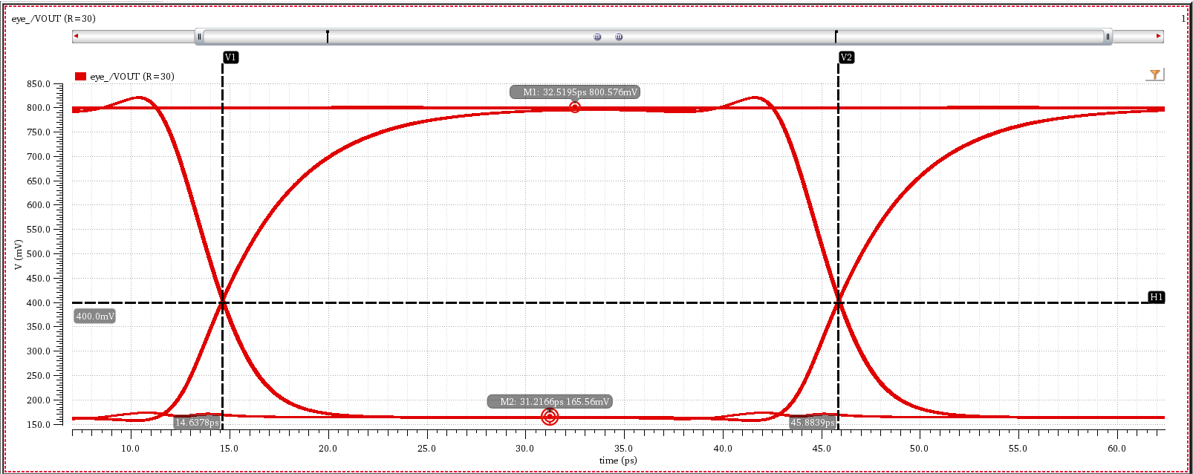
\includegraphics[width=1\textwidth]{cmleye.png}
    \caption{Simulated Eye Diagram of the Pseudo-CML topology at 64 Gb/s.}
    \label{fig:cml_eye}
\end{figure}

Figure \ref{fig:cml_eye} presents the eye diagram captured at the output node. The eye opening confirms that the resistive pull-up and active pull-down provide sufficient bandwidth for 64 Gb/s operation.

\begin{figure}[H]
    \centering
    % --- First Subfigure (Deterministic Jitter) ---
    \begin{subfigure}[b]{0.48\textwidth}
        \centering
        % Replace 'image_deterministic.png' with your actual filename
        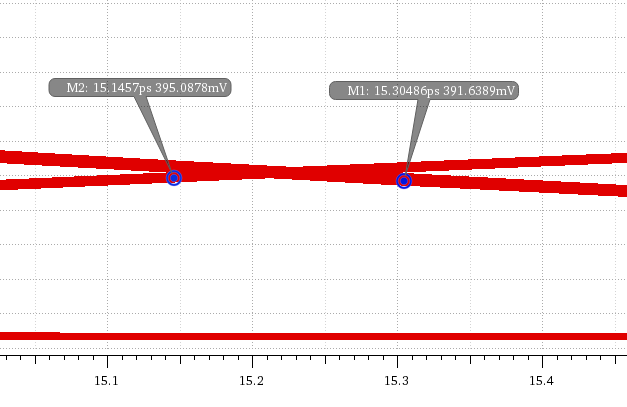
\includegraphics[width=\textwidth]{cml dj.png}
        \caption{Deterministic Jitter with clean supply}
        \label{fig:dj_zoom}
    \end{subfigure}
    \hfill % Adds flexible space between the images
    % --- Second Subfigure (Total Jitter) ---
    \begin{subfigure}[b]{0.6\textwidth}
        \centering
        % Replace 'image_total.png' with your actual filename
        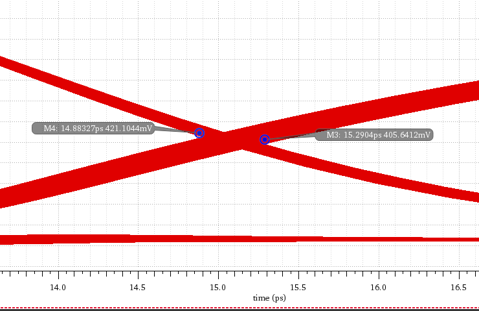
\includegraphics[width=\textwidth]{psij cml.png}
        \caption{Total Jitter with noisy supply}
        \label{fig:tj_zoom}
    \end{subfigure}
    
    \caption{Jitter measurement comparison showing (a) Deterministic Jitter components and (b) Total Jitter accumulation.}
    \label{fig:jitter_comparison}
\end{figure}

% ==================================================
% ==================================================
% CML SIMULATION METRICS SUMMARY
% ==================================================
\subsubsection{Simulation Metrics Summary}
\label{subsubsec:cml_sim_metrics}

Table \ref{tab:cml_metrics} summarizes the key performance indicators extracted from the schematic-level simulations of the Current Mode based topology at 64 Gb/s.

\begin{table}[H]
    \centering
    \caption{Summary of Simulated Performance Metrics for the Current Mode Topology (Schematic Level)}
    \label{tab:cml_metrics}
    \renewcommand{\arraystretch}{1.4}
    \setlength{\tabcolsep}{12pt}
    \begin{tabular}{|l|c|}
        \hline
        \textbf{Specification} & \textbf{Value} \\ \hline
        \textbf{Power (mW)} & 5.358 \\ \hline
        \textbf{Swing (mV)} & 634.44 \\ \hline
        \textbf{Eye width (ps)} & 30.84 \\ \hline
        \textbf{Eye Crossing (mV)} & 400 \\ \hline
        \textbf{Deterministic Jitter (fs)} & 159.1 \\ \hline
        \textbf{Power Supply Induced Jitter (fs)} & 248.03 \\ \hline
        \textbf{Total Jitter (fs)} & 407.13 \\ \hline
        \textbf{Eye rise time (ps)} & 9.1 \\ \hline
        \textbf{Eye fall time (ps)} & 4.905 \\ \hline
    \end{tabular}
\end{table}

The metrics in Table \ref{tab:cml_metrics} reveal the fundamental trade-offs associated with this topology:

\begin{itemize}
    \item \textbf{Comparable Power Consumption:} The power consumption of the CML driver (5.358 mW) is comparable to the Transmission Gate topology (5.883 mW). However, the nature of this dissipation is different: whereas the Transmission Gate topology is dominated by dynamic switching power, the CML topology consumes primarily static power dissipated across the load resistor when the output is active (Logic '0').
    
    \item \textbf{Reduced Output Swing:} The primary trade-off for this architecture is the reduced output swing. The CML driver achieves a swing of 634.44 mV, which is approximately 20\% lower than the rail-to-rail swing (799.8 mV) achieved by the Transmission Gate topology. This reduction is inherent to the resistive load design, where the low-level output voltage ($V_{OL}$) is non-zero.
    
    \item \textbf{Signal Integrity:} Despite the reduced swing, the driver maintains excellent signal integrity with an eye width of 30.84 ps and jitter (407.13 fs), validating that the static drive strength is sufficient for the target data rate.
\end{itemize}

\subsection{Topology C: Tri-State Inverter Implementation}
\label{subsec:tinv_impl}

The final topology evaluated is the Tri-State Inverter based driver. This architecture combines the signal driving capability of standard CMOS logic with the multiplexing functionality required for the Quarter-Rate transmitter. Unlike the Transmission Gate (which is a passive switch) or the CML driver (which is a resistive-load switch), the Tri-State inverter provides active drive for both logic '0' and logic '1' while supporting a high-impedance (Hi-Z) state for serialization.

\subsubsection{Circuit Implementation}
The circuit functions as a selectable driver slice. Unlike a conventional "stacked" tri-state inverter which puts gating transistors in series with the output (reducing voltage headroom), this topology uses a \textbf{Split-Path Pre-Driver} scheme to control a standard complementary output stage.

\begin{itemize}
    \item \textbf{Switch Structure:} The output stage consists of a single PMOS transistor ($P_0$) and a single NMOS transistor ($N_0$) connected to the output node ($V_{out}$). This minimizes the on-resistance and maximizes the output voltage swing since there are no stacked series switches.
    
    \item \textbf{Control Logic:} The tri-state functionality is achieved by independently controlling the gates of $P_0$ and $N_0$ using two parallel logic paths driven by the sampling clock ($CLK_0$).
    \begin{itemize}
        \item \textbf{PMOS Control Path:} The data ($D_0$) and clock ($CLK_0$) are inputs to an AND gate followed by an Inverter.
        \begin{itemize}
            \item When $CLK_0 = 1$ and $D_0 = 1$: The path outputs logic '0', turning the PMOS \textbf{ON} (Pull-Up).
        \end{itemize}
        \item \textbf{NMOS Control Path:} The inverted data ($D_{0\_bar}$) and clock ($CLK_0$) are inputs to an AND gate followed by a Transmission Gate (TG).
        \begin{itemize}
             \item When $CLK_0 = 1$ and $D_0 = 0$ (so $D_{0\_bar} = 1$): The path outputs logic '1', turning the NMOS \textbf{ON} (Pull-Down).
        \end{itemize}
    \end{itemize}

    \item \textbf{High Impedance State (Hi-Z):} When the slice is inactive ($CLK_0 = 0$), the control logic forces both output transistors into the cut-off region simultaneously.
    \begin{itemize}
        \item The top path outputs logic '1', turning the PMOS \textbf{OFF}.
        \item The bottom path outputs logic '0', turning the NMOS \textbf{OFF}.
        \item With both devices off, the output node is left floating (High-Z), allowing parallel active slices to drive the bus without contention.
    \end{itemize}
\subsubsection{Sizing Strategy (Delay Matching \& Symmetry)}
The sizing strategy for the Split-Path Tri-State topology required a two-stage optimization process to ensure both timing synchronization and drive strength symmetry.

\begin{itemize}
    \item \textbf{Step 1: Path Delay Equalization:}
    The primary challenge of the split-path architecture is that the PMOS control path includes an Inverter (logic inversion), while the NMOS control path is non-inverting. To compensate for the propagation delay introduced by the Inverter, a Transmission Gate (TG) was inserted into the NMOS path.
    \begin{itemize}
        \item The width of the transistors in the Transmission Gate was swept parametrically to tune its RC delay.
        \item The optimization goal was to match the arrival time of the control signals at the gates of PMOS and NMOS, ensuring simultaneous switching and minimizing short-circuit power during transitions.
    \end{itemize}

    \item \textbf{Step 2: Output Stage Symmetry ($V_M$ Centering):}
    Once the control signals were synchronized, the output transistors  were sized to achieve symmetric drive strength.
    \begin{itemize}
        \item Since the hole mobility ($\mu_p$) is lower than electron mobility ($\mu_n$), the PMOS width ($W_p$) was sized larger than the NMOS width ($W_n$) ($\mu_n$=1.6*$\mu_p$).
        \item The ratio $W_p/W_n$ was adjusted to so that ($W_p$=1.6*$W_n$).the Rise Time ($t_{rise}$) and Fall Time ($t_{fall}$) were approximately equal. This symmetry centers the switching threshold ($V_M$) at $V_{DD}/2$, maximizing the noise margins and horizontal eye opening.
    \end{itemize}
    
\end{itemize}
    \item \textbf{Delay Matching (TG vs. Inverter):} A critical design feature is the inclusion of the Transmission Gate in the NMOS control path. Since the PMOS path uses an Inverter (which adds propagation delay), the TG is inserted in the NMOS path to replicate this delay. This ensures that the drive signals arrive at the gates of output PMOS and NMOS simultaneously, minimizing crossover current and skew.
\end{itemize}
\begin{figure}[H]
    \centering
    % REPLACE 'tri_slice2.png' with your actual filename
    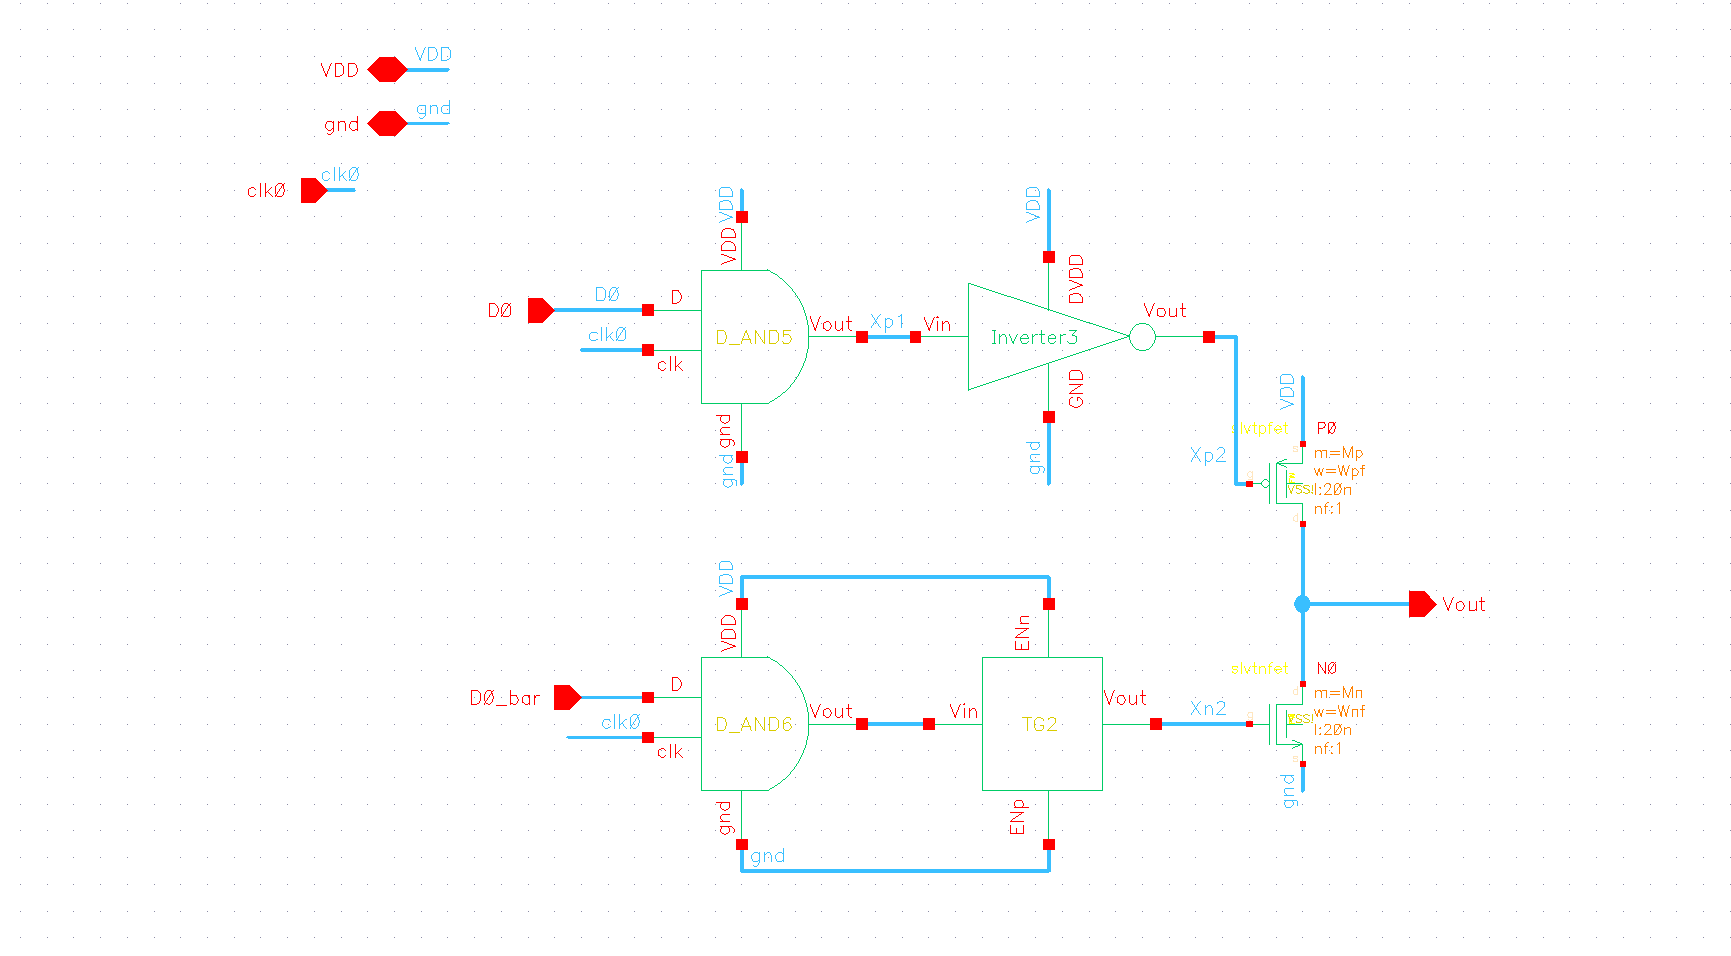
\includegraphics[width=0.8\textwidth]{tri_slice2.png}
    \caption{Schematic implementation of the Split-Path Tri-State driver. The design uses independent logic paths for the PMOS and NMOS devices. A Transmission Gate is inserted in the bottom path to match the delay of the Inverter in the top path.}
    \label{fig:tinvslice_schematic}
\end{figure}
\subsubsection{Simulation Results: Transient Response and Eye Diagram}
The functional verification of the Tri-State topology was performed at 64 Gb/s. The results demonstrate sharp, rail-to-rail transitions with minimal Inter-Symbol Interference (ISI).

\begin{figure}[htbp]
    \centering
    % REPLACE 'tinvout.png' with your filename
    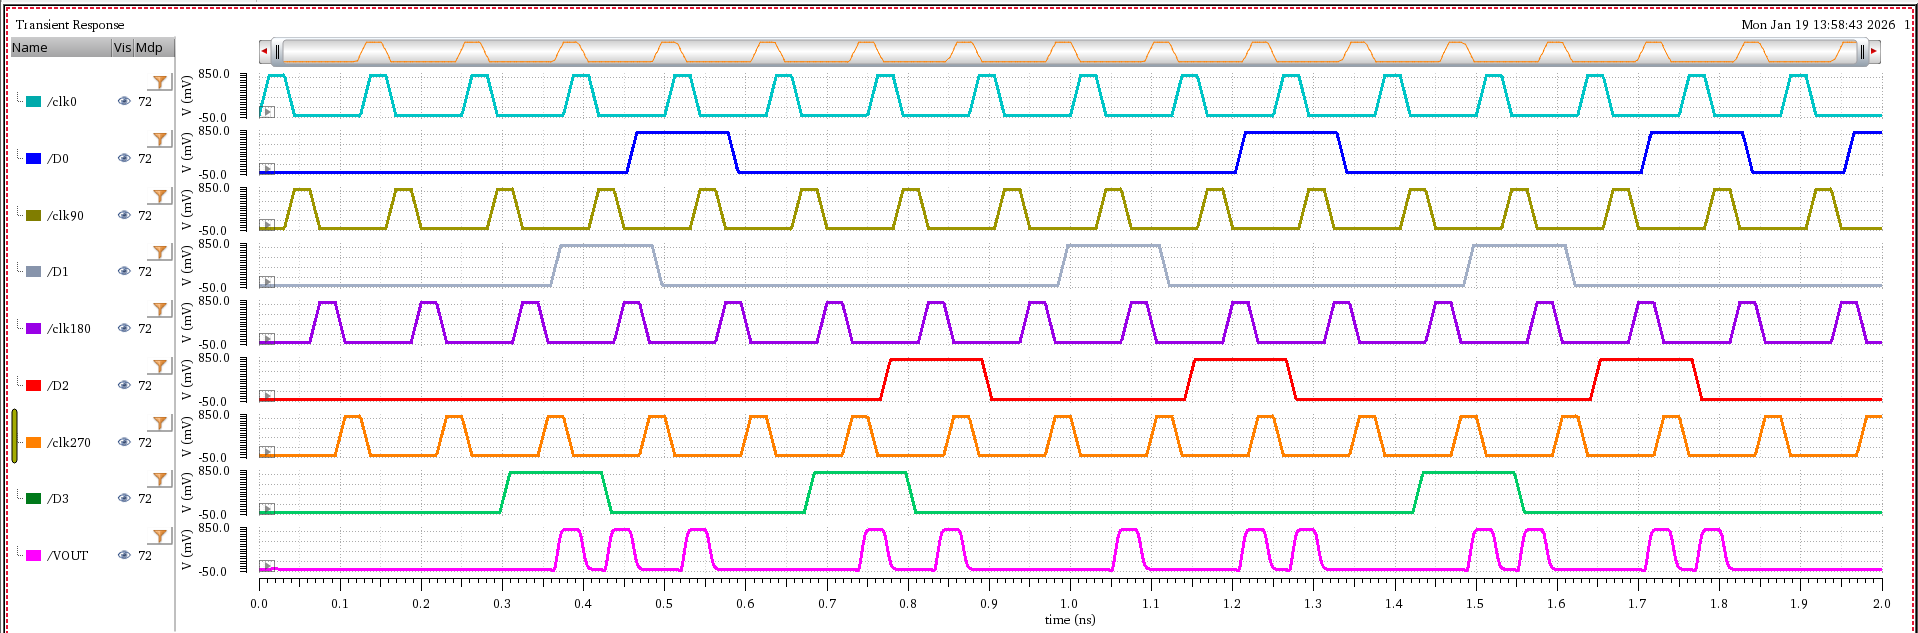
\includegraphics[width=1\textwidth]{tinvout_2n.png}
    \caption{Transient response of the Tri-State Inverter driver output at 64 Gb/s.}
    \label{fig:tinv_transient}
\end{figure}

Figure \ref{fig:tinv_transient} illustrates the transient response. The waveform shows full rail-to-rail switching with balanced rising and falling edges, validating the symmetric sizing strategy.

\begin{figure}[htbp]
    \centering
    % REPLACE 'tinveye.png' with your filename
    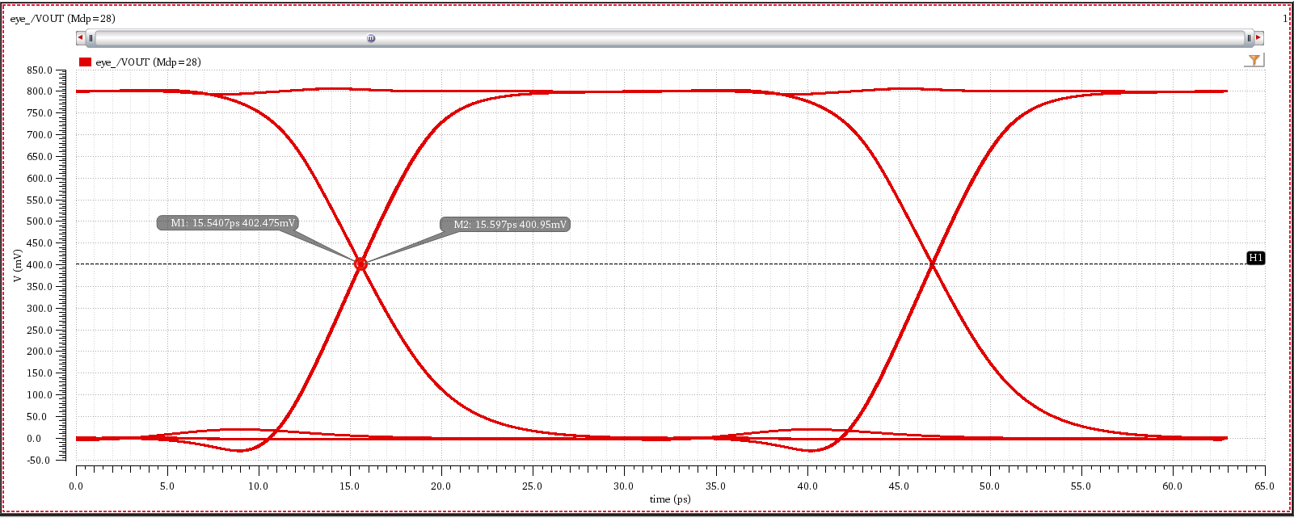
\includegraphics[width=1\textwidth]{tinveye.png}
    \caption{Simulated Eye Diagram of the Tri-State Inverter topology at 64 Gb/s.}
    \label{fig:tinv_eye}
\end{figure}

Figure \ref{fig:tinv_eye} presents the eye diagram. The Tri-State topology yields a very clean eye, benefiting from the active restoration of signal levels.

\begin{figure}[H]
    \centering
    % --- First Subfigure (Deterministic Jitter) ---
    \begin{subfigure}[b]{0.6\textwidth}
        \centering
        % Replace 'image_deterministic.png' with your actual filename
        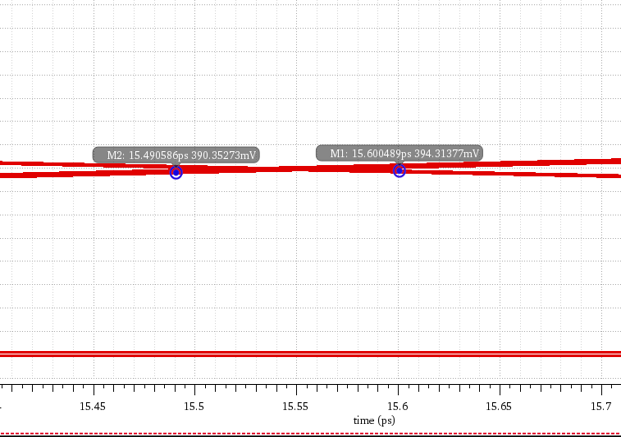
\includegraphics[width=\textwidth]{tri dj.png}
        \caption{Deterministic Jitter with clean supply}
        \label{fig:dj_zoom}
    \end{subfigure}
    \hfill % Adds flexible space between the images
    % --- Second Subfigure (Total Jitter) ---
    \begin{subfigure}[b]{0.6\textwidth}
        \centering
        % Replace 'image_total.png' with your actual filename
        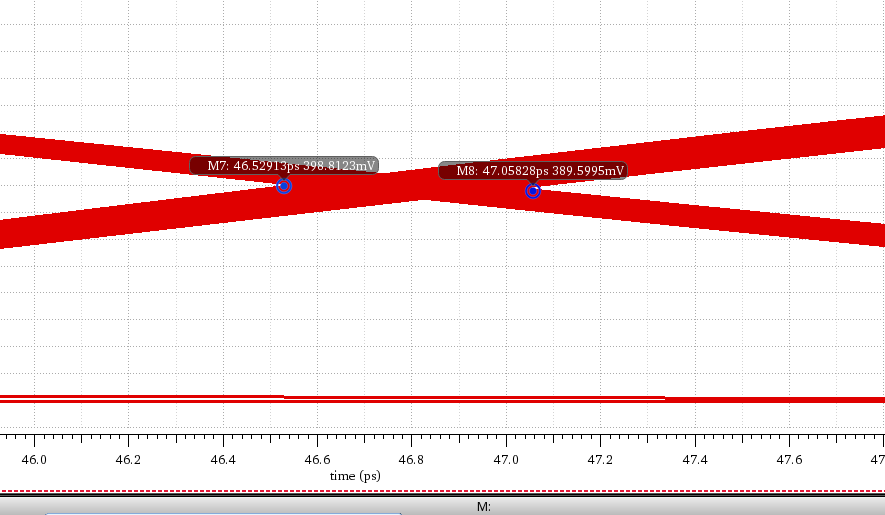
\includegraphics[width=\textwidth]{PSJ TRISTATE.png}
        \caption{Total Jitter with noisy supply}
        \label{fig:tj_zoom}
    \end{subfigure}
    
    \caption{Jitter measurement comparison showing (a) Deterministic Jitter components and (b) Total Jitter accumulation.}
    \label{fig:jitter_comparison}
\end{figure}
% ==================================================
% TRI-STATE SIMULATION METRICS SUMMARY
% ==================================================
\subsubsection{Simulation Metrics Summary}
\label{subsubsec:tinv_sim_metrics}

Table \ref{tab:tinv_metrics} summarizes the key performance indicators extracted from the schematic-level simulations of the Tri-State Inverter based topology at 64 Gb/s.

\begin{table}[H]
    \centering
    \caption{Summary of Simulated Performance Metrics for the Tri-State Inverter Topology (Schematic Level)}
    \label{tab:tinv_metrics}
    \renewcommand{\arraystretch}{1.4}
    \setlength{\tabcolsep}{12pt}
    \begin{tabular}{|l|c|}
        \hline
        \textbf{Specification} & \textbf{Value} \\ \hline
        \textbf{Power (mW)} & 4.076 \\ \hline
        \textbf{Swing (mV)} & 798.81 \\ \hline
        \textbf{Eye width (ps)} & 30.72 \\ \hline
        \textbf{Eye Crossing (mV)} & 403 \\ \hline
        \textbf{Deterministic Jitter (fs)} & 109.903 \\ \hline
        \textbf{Power Supply Induced Jitter (fs)} & 419.247 \\ \hline
        \textbf{Total Jitter (fs)} & 529.177 \\ \hline
        \textbf{Eye rise time (ps)} & 7.16 \\ \hline
        \textbf{Eye fall time (ps)} & 8.705 \\ \hline
    \end{tabular}
\end{table}

The metrics in Table \ref{tab:tinv_metrics} suggest that the Tri-State Inverter topology offers the most balanced performance profile among the evaluated architectures:

\begin{itemize}
    \item \textbf{Lowest Power Consumption:} At 4.076 mW, this topology consumes the least power. It avoids the static power dissipation of the CML driver (no resistor path to ground) and appears to manage dynamic switching more efficiently than the Transmission Gate implementation.
    
    \item \textbf{Rail-to-Rail Swing:} Like the Transmission Gate, it provides a full output swing of 798.81 mV, maximizing the Signal-to-Noise Ratio (SNR).
    
    \item \textbf{Symmetric Performance:} The rise time (7.16 ps) and fall time (8.705 ps) are closely matched, and the Eye Crossing is centered at 400 mV With total jitter (529.177 fs).
    
\end{itemize}

\subsection{Comparison and Topology Selection}
\label{subsec:topology_comparison}

This section presents a comparative analysis of the three evaluated driver topologies—Transmission Gate (TG), Pseudo-CML, and Tri-State Inverter. The comparison is based on the schematic-level simulation results obtained at a data rate of 64 Gb/s.

\subsubsection{Summary of Specifications}
Table \ref{tab:comparison_summary} aggregates the key performance metrics for all three topologies to facilitate direct comparison.

\begin{table}[H]
    \centering
    \caption{Performance Comparison of Driver Topologies at 64 Gb/s}
    \label{tab:comparison_summary}
    \renewcommand{\arraystretch}{1.3}
    \setlength{\tabcolsep}{6pt} % Slightly reduced to fit width if needed
    \begin{tabular}{|l|c|c|c|}
        \hline
        \textbf{Specification} & \textbf{Transmission Gate} & \textbf{Tri-State Inverter} & \textbf{Current Mode (CML)} \\ \hline
        \textbf{Power (mW)} & 5.883 & 4.076 & 5.358 \\ \hline
        \textbf{Swing (mV)} & 799.8 & 798.81 & 634.44 \\ \hline
        \textbf{Eye width (ps)} & 30.66 & 30.72 & 30.84 \\ \hline
        \textbf{Eye Crossing (mV)} & 387.255 & 403 & 400 \\ \hline
        \textbf{Deterministic Jitter (fs)} & 255.77 & 109.903 & 159.1 \\ \hline
        \textbf{PSIJ (fs)} & 185.59 & 419.247 & 248.03 \\ \hline
        \textbf{Total Jitter (fs)} & 441.36 & 529.177 & 407.13 \\ \hline
        \textbf{Eye rise time (ps)} & 8 & 7.16 & 9.1 \\ \hline
        \textbf{Eye fall time (ps)} & 8 & 8.705 & 4.905 \\ \hline
    \end{tabular}
\end{table}

\subsubsection{Performance Comparison}

\textbf{1. Power Consumption:}
The simulations reveal a significant divergence in power efficiency:
\begin{itemize}
    \item The \textbf{Transmission Gate} topology exhibited the highest power consumption (5.883 mW). This is attributed to the substantial buffering power required to toggle the large transmission gate switches at 32 GHz.
    \item The \textbf{Pseudo-CML} topology showed moderate power consumption (5.358 mW). While it simplifies the logic path, it suffers from unavoidable static power dissipation across the load resistor whenever the output is active.
    \item The \textbf{Tri-State Inverter} achieved the lowest power consumption (4.076 mW). It achieves these superior results by eliminating static currents while maintaining high drive efficiency.
\end{itemize}

\textbf{2. Output Swing and Signal Integrity:}
\begin{itemize}
    \item Both the \textbf{Transmission Gate} and \textbf{Tri-State Inverter} achieved full rail-to-rail output swings ($\approx 800$ mV), maximizing the Vertical eye opening and Signal-to-Noise Ratio (SNR).
    \item The \textbf{Pseudo-CML} topology is limited to a reduced swing of 634.44 mV due to the resistive voltage division required to set $V_{OL}$. This reduced swing makes this topology sensitive to Process, Voltage, and Temperature (PVT) variations.
\end{itemize}

\textbf{3. Timing Symmetry and Jitter:}
\begin{itemize}
    \item The \textbf{Tri-State Inverter} shows reasonable symmetry ($t_{rise} \approx 7.16$ ps, $t_{fall} \approx 8.7$ ps) and the lowest Deterministic Jitter (109.9 fs). The Eye Crossing is centered at 403 mV, ensuring maximum horizontal eye opening.
    \item The \textbf{Transmission Gate} shows perfect symmetry (8 ps Rise / 8 ps Fall) but generally slower edges compared to the Tri-State's rise time.
    \item The \textbf{Pseudo-CML} driver exhibited inherent asymmetry ($t_{rise}=9.1$ ps vs $t_{fall}=4.9$ ps) because the rising edge is passive (RC limited) while the falling edge is active.
    \item \textbf{Power Supply Induced Jitter (PSIJ):} A distinct trade-off was observed regarding supply noise. The \textbf{Tri-State Inverter} exhibited the highest sensitivity to supply ripple (PSIJ $\approx 419$ fs) due to its active rail-dependent switching. In contrast, the \textbf{Transmission Gate} topology proved the most robust against supply noise (PSIJ $\approx 185.6$ fs). However, the Tri-State was still selected for its superior intrinsic jitter performance (lowest Deterministic Jitter).
\end{itemize}
\subsubsection{Final Topology Selection}
Based on the data presented in Table \ref{tab:comparison_summary} and the analysis above, the \textbf{Tri-State Inverter} is selected as the optimal topology for the Quarter-Rate transmitter.

\textbf{Justification:}
\begin{enumerate}
    \item \textbf{Efficiency:} It offers the lowest power consumption (4.076mW), outperforming both the Transmission Gate and CML topologies.
    \item \textbf{Robustness:} It provides the maximum possible voltage swing (798.81 mV) and the lowest Deterministic Jitter (109.9 fs), ensuring superior intrinsic timing stability despite its higher sensitivity to supply noise.
    \item \textbf{Signal Quality:} The drive strength results in a near-perfectly centered eye crossing (403 mV), which is critical to minimize ISI in high-speed links.
\end{enumerate}

\textbf{Consequently, the  Tri-State Inverter based Mux will be the best to move on with.}
\clearpage
\section{Driver}
\subsection{SST implementation}
\subsubsection{Circuit implementation}
\begin{figure}[H]
     \centering
     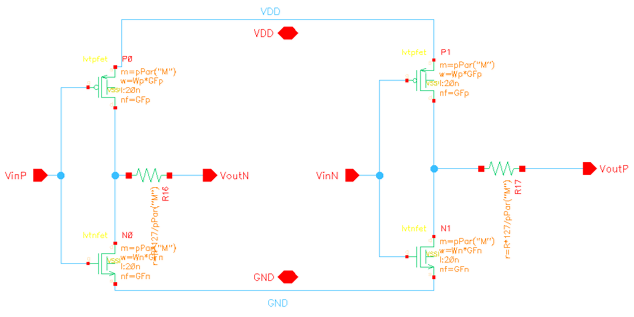
\includegraphics[width=0.7\textwidth]{19)schSST}
     \caption{Slice schematic}
 \end{figure}
 \begin{figure}[H]
     \centering
     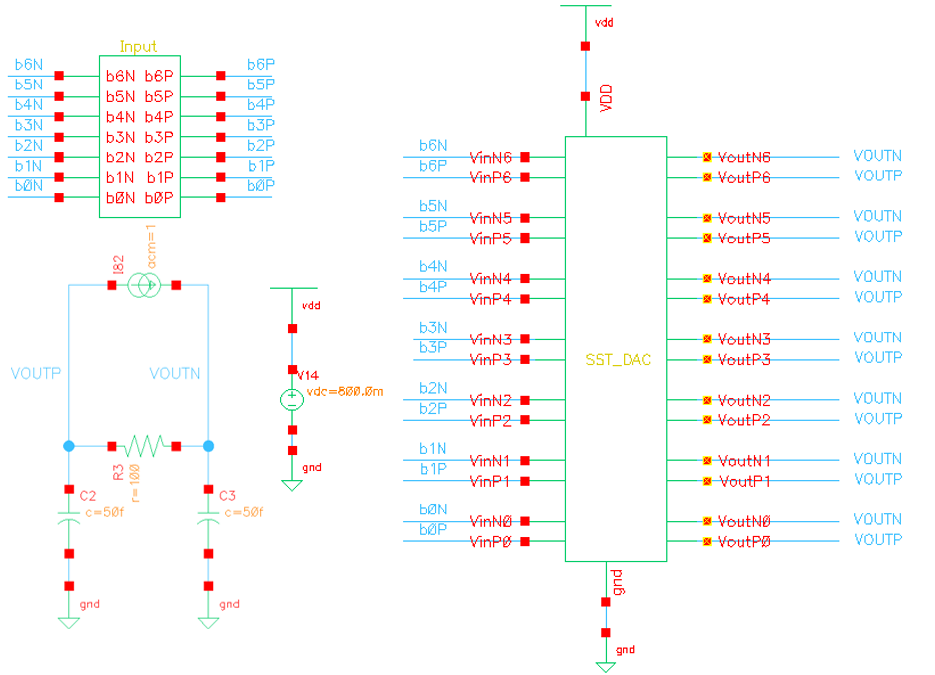
\includegraphics[width=0.7\textwidth]{19.1)DACsstTB}
     \caption{DAC TB}
 \end{figure}
  \begin{itemize}
 \item The 7b DAC consists of 7 slices where each slice is weighted by pPar(“M”) acc to bit weight
\item So for each slice : Width of transistor = (Wtotal/127) * pPar(“M”)  and R[series]=(35*127)/ pPar(“M”) 
 \end{itemize}
 
\subsubsection{Design Knobs/Sizing}
\begin{figure}[H]
     \centering
     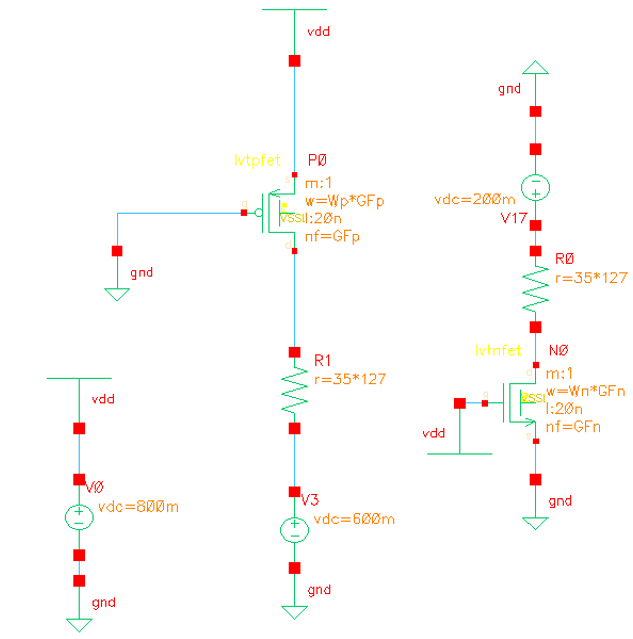
\includegraphics[width=0.5\textwidth]{19.2)sizingTB}
     \caption{Sizing TB}
 \end{figure}
 
\begin{figure}[H]
    \centering
    % --- Subfigure (a) ---
    \begin{subfigure}{0.48\linewidth}
        \centering
        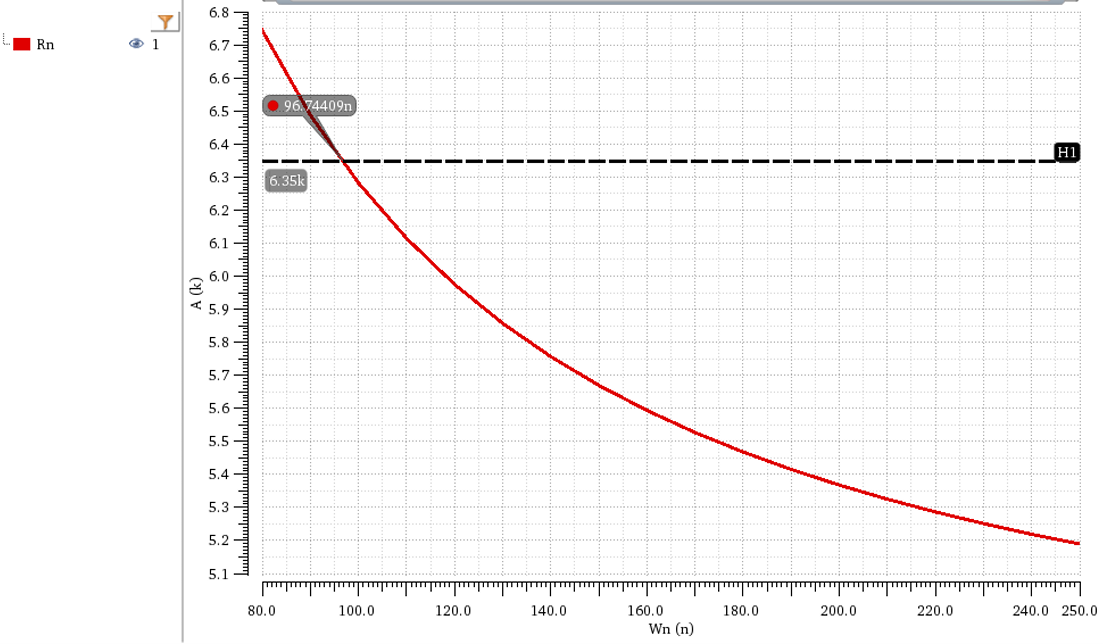
\includegraphics[width=\textwidth]{19.3)Nfetwidth}
        \caption{}
    
    \end{subfigure}
    \hfill
    % --- Subfigure (b) ---
    \begin{subfigure}{0.5\linewidth}
        \centering
        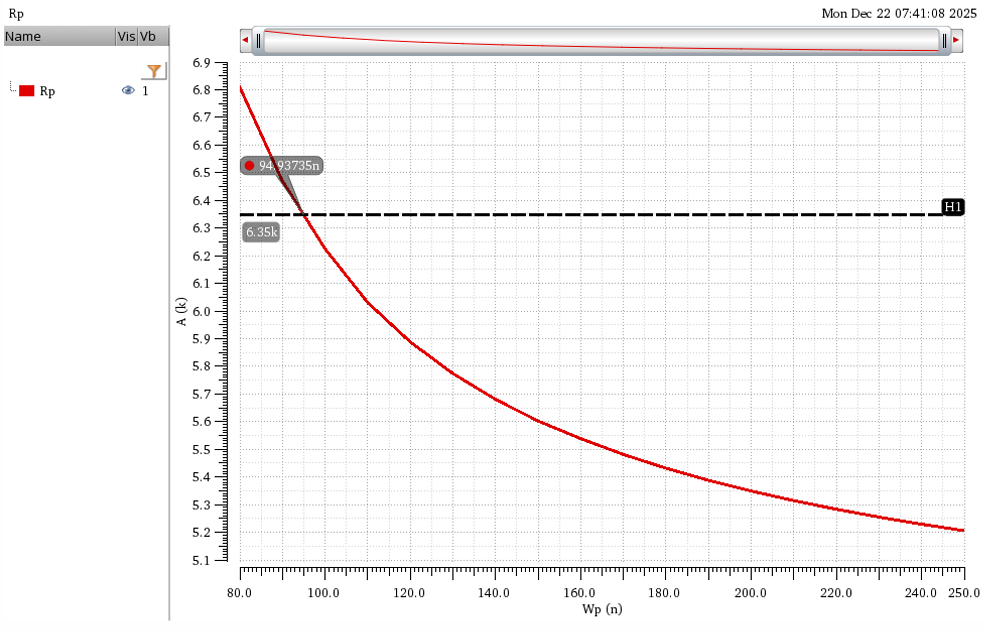
\includegraphics[width=\textwidth]{19.4)PfetWidth}
        \caption{}
    \end{subfigure}
    \hfill
    \vspace{0.3cm}
    \caption{ (a) NFET Width ; (b) PFET Width}
\end{figure}

   \begin{itemize}
 \item We have sizing tradeoffs :
    \begin{itemize}
    \item  increase R[series] w.r.t. RON but this will increase transistors’ sizes so degrades BW
    \item  increase RON but this will degrade linearity
     \end{itemize}
\item  I chose R[series] to be $35\,\Omega$ so RON will be $15\,\Omega$ (ratio is 70\% to 30\%) 
 \end{itemize}
\subsubsection{Results}
\begin{figure}[H]
     \centering
     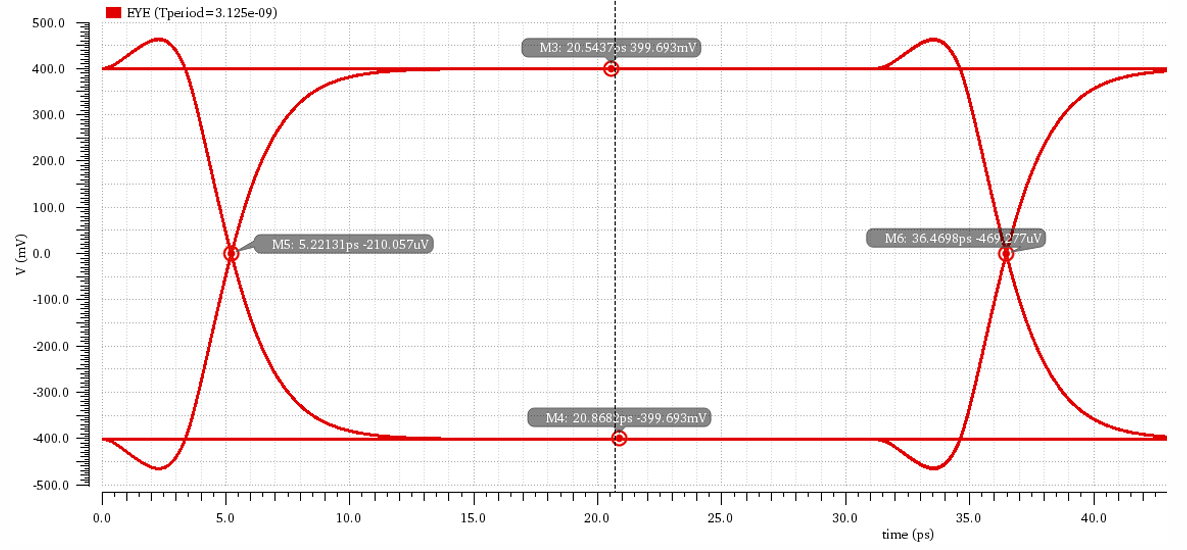
\includegraphics[width=0.7\textwidth]{21)NRZswingSST}
     \caption{NRZ Swing}
 \end{figure}
 PP Differential Swing = 799.4mV
 UI = 31.2485ps
 
 \begin{figure}[H]
     \centering
     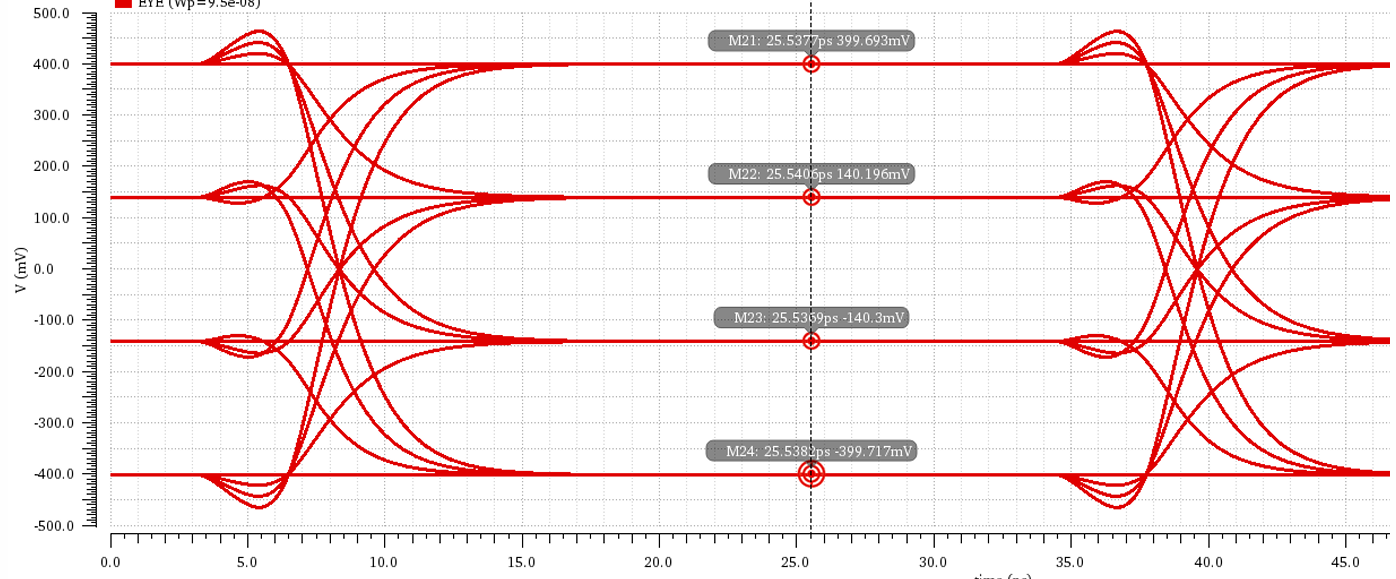
\includegraphics[width=0.7\textwidth]{21.1)PAM4swingSST}
     \caption{PAM4 Swing}
 \end{figure}
 
 \begin{align*}
    S_{min} &= \min(V3 - V2, V2 - V1, V0) \\
    RLM &= \frac{3 \times S_{min}}{V3 - V0} = 97.5\%
\end{align*}

\subsection{CML implementation}
\subsubsection{Circuit implementation}

\begin{figure}[H]
    \centering
    % --- Subfigure (a) ---
    \begin{subfigure}{0.48\linewidth}
        \centering
        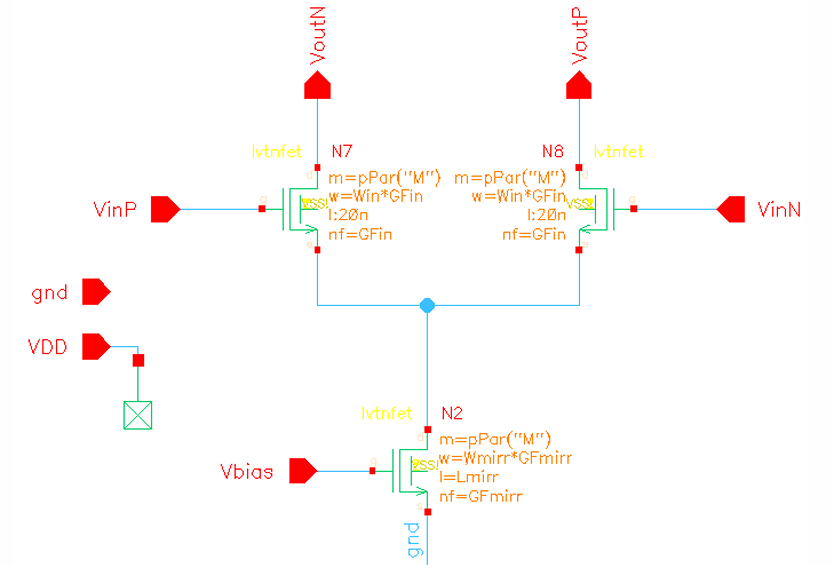
\includegraphics[width=\textwidth]{20)CMLslice1}
        \caption{}
    
    \end{subfigure}
    \hfill
    % --- Subfigure (b) ---
    \begin{subfigure}{0.5\linewidth}
        \centering
        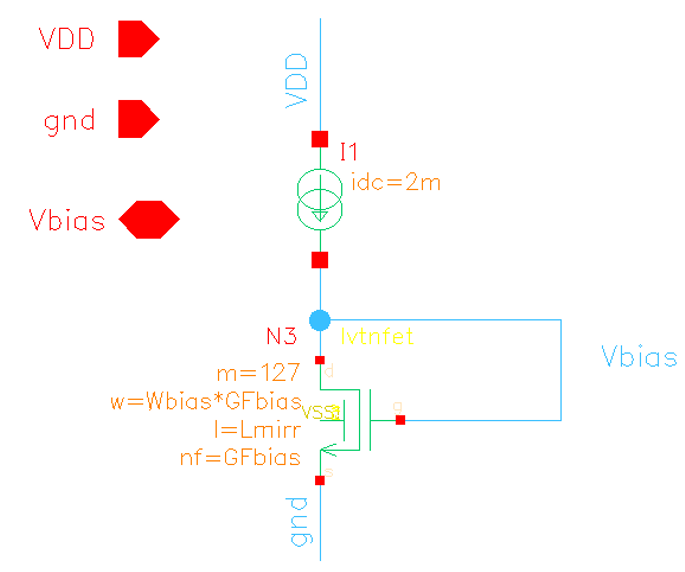
\includegraphics[width=\textwidth]{20.1)CMLslice2}
        \caption{}
    \end{subfigure}
    \hfill
    \vspace{0.3cm}
    \caption{ (a) Schematic ; (b) Biasing}
\end{figure}
 \begin{figure}[H]
     \centering
     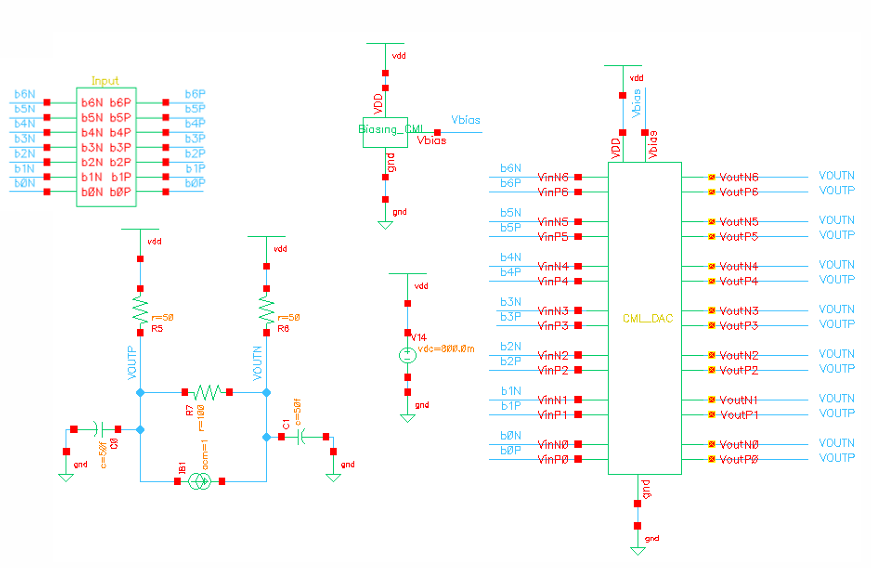
\includegraphics[width=0.7\textwidth]{20.2)DCAcmlTB}
     \caption{DAC TB}
 \end{figure}


\subsubsection{Design Knobs/Sizing}
\begin{figure}[H]
     \centering
     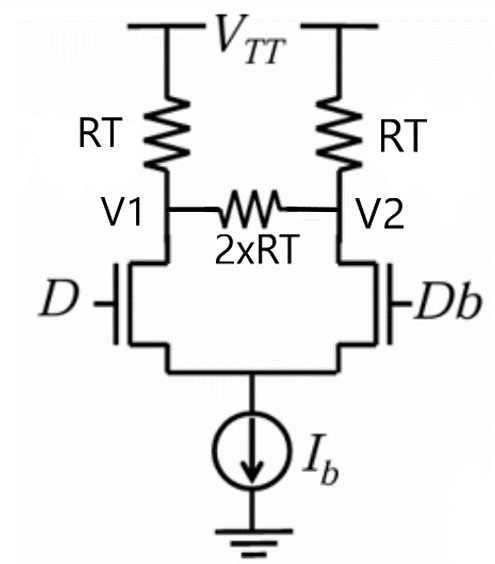
\includegraphics[width=0.4\textwidth]{ 20.3)desknobcir}
     \caption{}
 \end{figure}
\begin{itemize}
    \item For diff termination: At $D=V_{DD}, D_b=0 \rightarrow V_1 = V_{DD} - \frac{3}{4} I_b \times R_T = 0.65V, V_2 = V_{DD} - \frac{1}{4} I_b \times R_T = 0.75V$
    \item I'm concerned with $V_1$ as $M_{db}$ is OFF So $0.65V$ is distributed on the i/p and the tail current source
    \item For tail current source: $W \uparrow, V_{ov} \downarrow, V_{DS}-V_{ov} \uparrow$, deeper into sat
    \item $V_{GS}$ i/p $\uparrow, V_{DS}$ tail $\downarrow, V_{DS}$ i/p $\uparrow, r_o$ i/p $\uparrow$ (this is achieved by $W$ i/p $\downarrow$)
    \item Swing $\downarrow, V_{oCM} \uparrow$, higher $V_{DS}s$
    \item \textcolor{red}{Why it is impossible to make CML with PP swing = $V_{DD}$ ?}
    \item $\rightarrow$ You don't have any headroom, and i/p pair will always in triode as $V_D = 0.8 - 0.75 \times 0.8 = 0.2V$ and $V_G = 0.8$
    \item $V_D$ must be $> V_G - V_T$ and this is impossible, so i/p pair will be in triode having low $r_o$ which isn't compatible with CML driver
\end{itemize}
\begin{figure}[H]
     \centering
     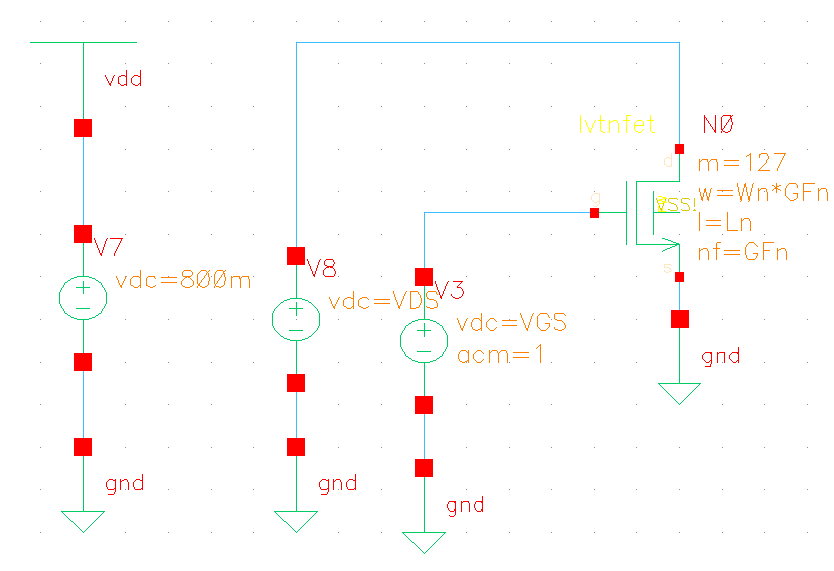
\includegraphics[width=0.7\textwidth]{ 20.4)sizingtbcml}
     \caption{Sizing TB}
 \end{figure}
 \begin{figure}[H]
    \centering
    % --- Subfigure (a) ---
    \begin{subfigure}{0.48\linewidth}
        \centering
        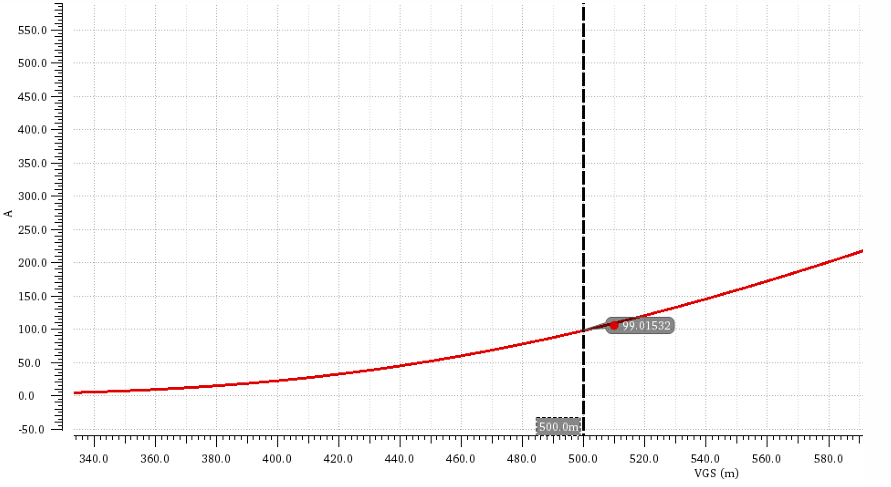
\includegraphics[width=\textwidth]{20.5)IDwippair}
        \caption{}
    
    \end{subfigure}
    \hfill
    % --- Subfigure (b) ---
    \begin{subfigure}{0.5\linewidth}
        \centering
        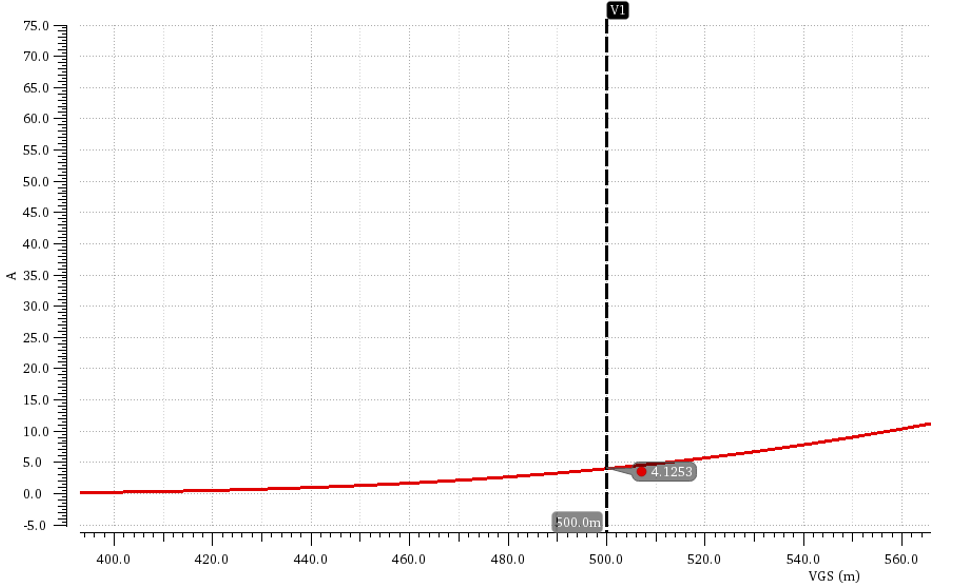
\includegraphics[width=\textwidth]{20.6)idwtail}
        \caption{}
    \end{subfigure}
    \hfill
    \vspace{0.3cm}
    \caption{ (a) ID/W (i/p pair) ; (b) ID/W (Tail)}
\end{figure}
\begin{itemize}
    \item We can distribute $0.65V$ as $0.35V$ for i/p and $0.3V$ for tail, so $V_{GSi/p} = 0.8-0.3=0.5V$
    \item For Tail, choose high $L$ ($300n$) it gives $V_{TH} \sim 450mV$ so make $V_{GS}=500mV$ so $50mV$ $v_{ov}$ and $300mV$ $V_{DS}$
    \item Get $W$ from id/w curve by $\frac{4m}{127 \times \frac{ID}{W}}$
    \item $W_{inp} = 300n, L_{in} = 20n, W_{tail} = 8u, L_{tail} = 300n$
\end{itemize}
\subsubsection{Results}
\begin{figure}[H]
     \centering
     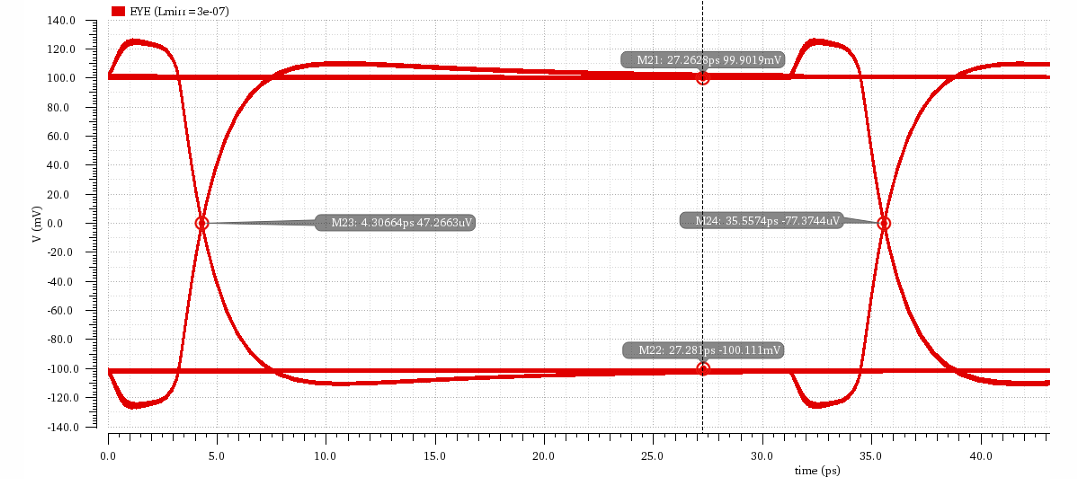
\includegraphics[width=0.7\textwidth]{22)NRZswingCML}
     \caption{NRZ Swing}
 \end{figure}
 PP Differential Swing ~ 200mV
 UI = 31.248ps
 
 \begin{figure}[H]
     \centering
     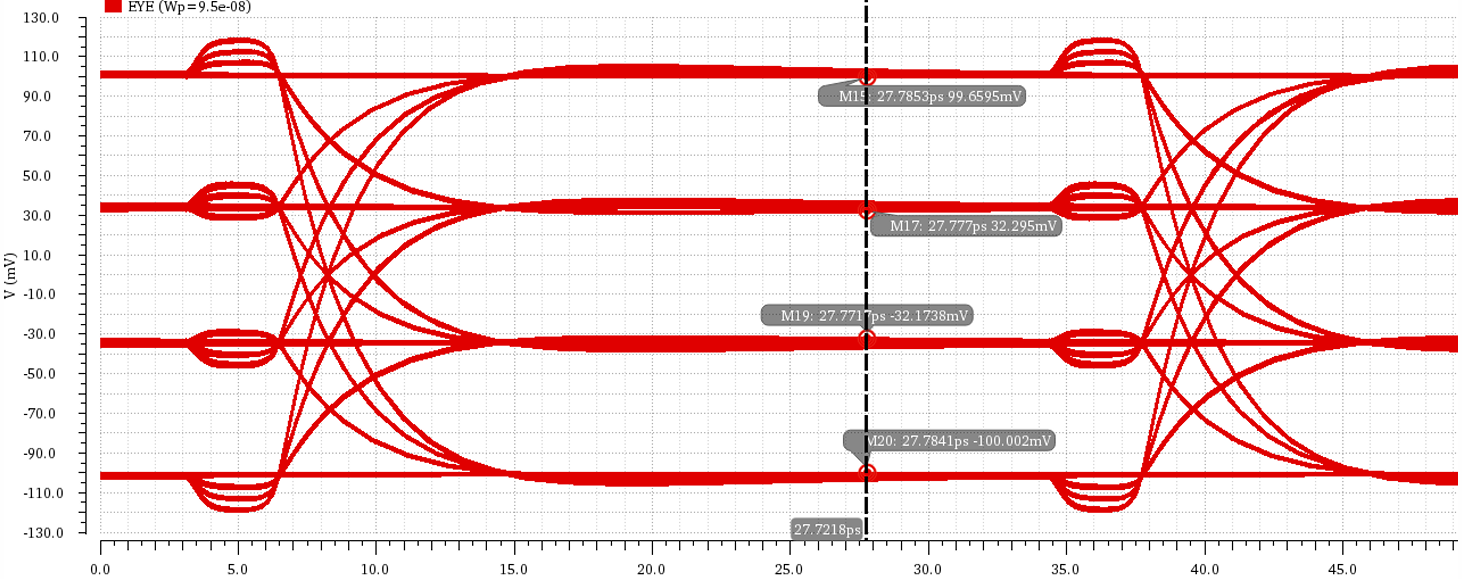
\includegraphics[width=0.7\textwidth]{22.1)PAM4SwingCML}
     \caption{PAM4 Swing}
 \end{figure}
 
 \begin{align*}
    S_{min} &= \min(V3 - V2, V2 - V1, V0) \\
    RLM &= \frac{3 \times S_{min}}{V3 - V0} =96\%
\end{align*}

\subsection{Comparison}

\begin{table}[htbp]
    \centering
    \caption{Final Comparative Performance Summary of SST and CML Drivers}
    \label{tab:final_performance_comparison}
    \begin{tabularx}{\textwidth}{l *{2}{X} *{2}{X}}
        \toprule
        & \multicolumn{2}{c}{\textbf{SST}} & \multicolumn{2}{c}{\textbf{CML}} \\
        \cmidrule(lr){2-3} \cmidrule(lr){4-5}
        \textbf{Modulation} & \textbf{NRZ} & \textbf{PAM-4} & \textbf{NRZ} & \textbf{PAM-4} \\
        \midrule
        Swing (pp) & \multicolumn{2}{c}{$799.4\,$mV} & \multicolumn{2}{c}{$200\,$mV} \\
        RLM & -- & $97.5\%$ & -- & $96\%$ \\
        Power & $3.48\,$mW & $4.581\,$mW & $4.8\,$mW & $4.8\,$mW \\
        Termination & \multicolumn{2}{c}{$49.3\,\Omega$} & \multicolumn{2}{c}{$49.7\,\Omega$} \\
        \bottomrule
    \end{tabularx}
\end{table}

\subsection{Verilog-A Codes}
\subsubsection{PAM4-input}

\begin{lstlisting}[caption={Verilog-A Implementation for PAM-4 Input Mapping}, label={lst:veriloga_pam4}]
`include "constants.vams"
`include "disciplines.vams"

module PAM4_input (in_msb, in_lsb, b0P, b0N, b1P, b1N, b2P, b2N, b3P, b3N, b4P, b4N, b5P, b5N, b6P, b6N);
    input in_msb, in_lsb;
    electrical in_msb, in_lsb;
    output b0P, b0N, b1P, b1N, b2P, b2N, b3P, b3N, b4P, b4N, b5P, b5N, b6P, b6N;
    electrical b0P, b0N, b1P, b1N, b2P, b2N, b3P, b3N, b4P, b4N, b5P, b5N, b6P, b6N;

    parameter real vdd = 0.8;
    parameter real vth = 0.4;
    parameter real trise = 3.125p;
    parameter real tfall = 3.125p;

    real b[0:6];
    integer i;

    analog begin
        // Mapping logic for PAM-4 levels
        if (V(in_msb) < vth && V(in_lsb) < vth) begin
            // Input 00 -> Pattern 0000000
            for (i=0; i<=6; i=i+1) b[i] = 0.0;
        end else if (V(in_msb) < vth && V(in_lsb) > vth) begin
            // Input 01 -> Pattern 0101010
            b[0]=0.0; b[1]=vdd; b[2]=0.0; b[3]=vdd; b[4]=0.0; b[5]=vdd; b[6]=0.0;
        end else if (V(in_msb) > vth && V(in_lsb) < vth) begin
            // Input 10 -> Pattern 1010101
            b[0]=vdd; b[1]=0.0; b[2]=vdd; b[3]=0.0; b[4]=vdd; b[5]=0.0; b[6]=vdd;
        end else begin
            // Input 11 -> Pattern 1111111
            for (i=0; i<=6; i=i+1) b[i] = vdd;
        end

        // Differential Output Drive
        V(b0P) <+ transition(b[0], 0, trise, tfall); V(b0N) <+ transition(vdd - b[0], 0, trise, tfall);
        V(b1P) <+ transition(b[1], 0, trise, tfall); V(b1N) <+ transition(vdd - b[1], 0, trise, tfall);
        V(b2P) <+ transition(b[2], 0, trise, tfall); V(b2N) <+ transition(vdd - b[2], 0, trise, tfall);
        V(b3P) <+ transition(b[3], 0, trise, tfall); V(b3N) <+ transition(vdd - b[3], 0, trise, tfall);
        V(b4P) <+ transition(b[4], 0, trise, tfall); V(b4N) <+ transition(vdd - b[4], 0, trise, tfall);
        V(b5P) <+ transition(b[5], 0, trise, tfall); V(b5N) <+ transition(vdd - b[5], 0, trise, tfall);
        V(b6P) <+ transition(b[6], 0, trise, tfall); V(b6N) <+ transition(vdd - b[6], 0, trise, tfall);
    end
endmodule
\end{lstlisting}
\begin{figure}[H]
     \centering
     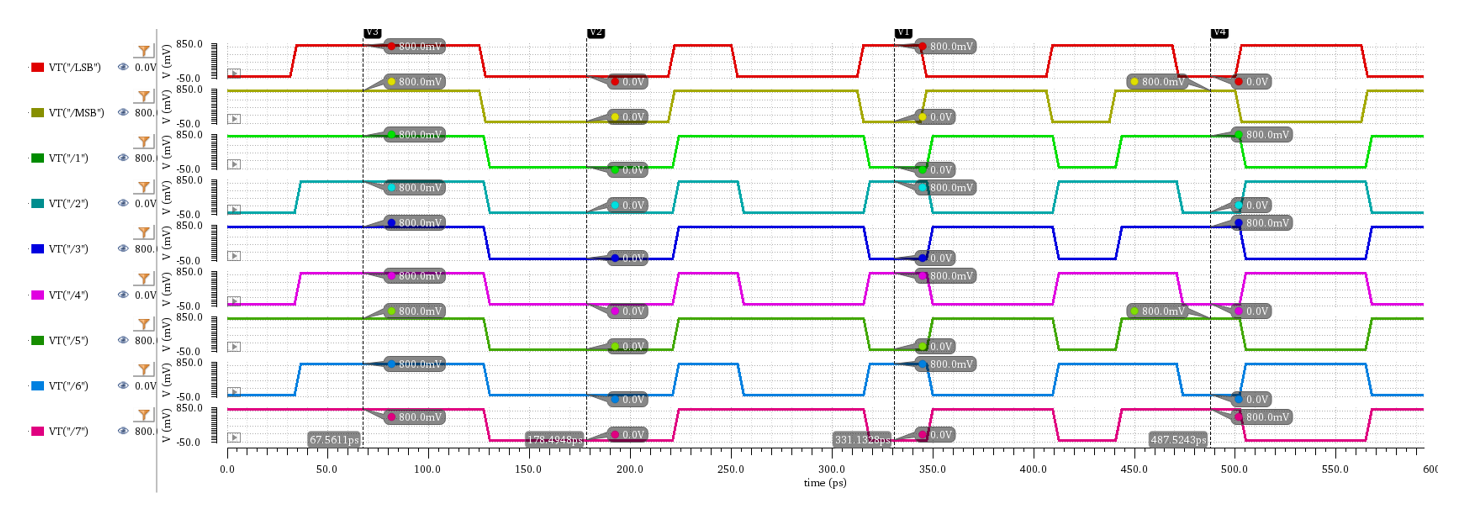
\includegraphics[width=1\textwidth]{23)PAM4code}
     \caption{Code testing}
 \end{figure}


\begin{table}[htbp]
    \centering
    \caption{PAM-4 Level Implementation using 7-bit Verilog-A Mapping}
    \label{tab:pam4_veriloga_mapping}
    \begin{tabular}{l l l l l l}
        \toprule
        \textbf{Level} & \textbf{Swing (VDD)} & \textbf{Ideal Code} & \textbf{Actual Code} & \textbf{Quantized V} & \textbf{Error} \\
        \midrule
        $+1/2 \times \text{Swing}$ & $+400.0\,$mV & $127.00$ & $127$ ($1111111$) & $+400.0\,$mV & $0.0\,$mV \\
        $+1/6 \times \text{Swing}$ & $+133.3\,$mV & $84.67$ & $85$ ($1010101$) & $+135.4\,$mV & $+2.1\,$mV \\
        $-1/6 \times \text{Swing}$ & $-133.3\,$mV & $42.33$ & $42$ ($0101010$) & $-135.4\,$mV & $-2.1\,$mV \\
        $-1/2 \times \text{Swing}$ & $-400.0\,$mV & $0.00$ & $0$ ($0000000$) & $-400.0\,$mV & $0.0\,$mV \\
        \bottomrule
    \end{tabular}
\end{table}








\end{document}